% !TeX document-id = {aa065125-16aa-457a-9e29-96da97cf31f1}
% !TEX TS-program = XeLaTeX
% Command for running this example (needs latexmkrc file):
%    latexmk -bibtex -pdf main.tex

%	نمونه پایان‌نامه آماده شده با استفاده از کلاس tehran-thesis، نگارش 1
%	سینا ممکن، دانشگاه تهران 
%	https://github.com/sinamomken/tehran-thesis
%	گروه پارسی‌لاتک
%	http://www.parsilatex.com
%	این نسخه، بر اساس نسخه‌ 0.1 از کلاس IUST-Thesis آقای محمود امین‌طوسی آماده شده است.
%        http://profsite.sttu.ac.ir/mamintoosi

%----------------------------------------------------------------------------------------------
% اگر قصد نوشتن پروژه کارشناسی را دارید، در خط زیر به جای msc، کلمه bsc و اگر قصد نوشتن رساله دکترا را دارید، کلمه phd را قرار دهید. کلیه تنظیمات لازم، به طور خودکار، اعمال می‌شود.

% اگر مایلید پایان‌نامه شما دورو باشد به جای oneside در خط زیر از twoside استفاده کنید.

% برای حاشیه‌نویسی و کم کردن صفحات ابتدایی، گزینه draft را وارد و برای نسخه نهایی آن را حذف کنید.

% برای استفاده از قلم‌های سری IR Series گزینه irfonts را وارد و برای استفاده از قلم‌های X Series 2 آن را حذف کنید.

\documentclass[
twoside
,openany
,phd
,irfonts
% ,draft
]{./tex/tehran-thesis}

% فایل commands.tex را مطالعه کنید؛ چون دستورات مربوط به فراخوانی بسته‌ها، فونت و دستورات خاص در این فایل قرار دارد.
% در این فایل، دستورها و تنظیمات مورد نیاز، آورده شده است.
%-------------------------------------------------------------------------------------------------------------------
% دستوراتی که پوشه پیش‌فرض زیرفایل‌های tex را مشخص می‌کند.
%\makeatletter
%\def\input@path{{./tex/}}
%\makeatother
% در ورژن جدید زی‌پرشین برای تایپ متن‌های ریاضی، این سه بسته، حتماً باید فراخوانی شود
\usepackage{amsthm,amssymb,amsmath}
% بسته‌ای برای تنطیم حاشیه‌های بالا، پایین، چپ و راست صفحه
\usepackage[top=40mm, bottom=40mm, left=25mm, right=35mm]{geometry}
% بسته‌‌ای برای ظاهر شدن شکل‌ها و تعیین آدرس تصاویر
\usepackage[final]{graphicx}
\graphicspath{{./img/}}
% بسته‌های مورد نیاز برای نوشتن کدها، رنگ‌آمیزی آنها و تعیین پوشهٔ کدها
\usepackage[final]{listings}
\usepackage[usenames,dvipsnames,svgnames,table]{xcolor}
\lstset{inputpath=./code/}
% بسته‌ای برای رسم کادر
\usepackage{framed} 
% بسته‌‌ای برای چاپ شدن خودکار تعداد صفحات در صفحه «معرفی پایان‌نامه»
\usepackage{lastpage}
% بسته‌ٔ لازم برای: ۱. تغییر شماره‌گذاری صفحات پیوست. ۲. تصحیح باگ آدرس وب حاوی '%' در مراجع
\usepackage{etoolbox}
%\usepackage{algpseudocode}
%\usepackage{algorithm}
\usepackage{algorithm}
\usepackage[noend]{algpseudocode}
%\usepackage{algorithmic}


%%%%%%%%%%%%%%%%%%%%%%%%%%%%%%%%%%%%
%%% دستورات وابسته به استیل مراجع:
%% اگر از استیل‌های natbib (plainnat-fa، asa-fa، chicago-fa) استفاده می‌کنید، خط زیر را فعال و بعدی‌اش را غیرفعال کنید.
%\usepackage{natbib}
%\newcommand{\citelatin}[1]{\cite{#1}\LTRfootnote{\citeauthor*{#1}}}
%\newcommand{\citeplatin}[1]{\citep{#1}\LTRfootnote{\citeauthor*{#1}}}
%% اگر از سایر استیل‌ها استفاده می‌کنید، خط بالا را غیرفعال و خط‌های زیر را فعال کنید.
\let\citep\cite
\let\citelatin\cite
\let\citeplatin\cite
%%%%%%%%%%%%
% بررسی حالت پیش نویس
\usepackage{ifdraft}
\ifdraft
{%
	% بسته‌ٔ ایجاد لینک‌های رنگی با امکان جهش
	\usepackage[unicode=true,pagebackref=true,
colorlinks,linkcolor=blue,citecolor=blue,final]{hyperref}
	%\usepackage{todonotes}
	\usepackage[firstpage]{draftwatermark}
	\SetWatermarkText{\ \ \ پیش‌نویس}
	\SetWatermarkScale{1.2}
}
{ 
	\usepackage[pagebackref=false,colorlinks,
	linkcolor=blue,citecolor=blue,urlcolor=blue]{hyperref}
	%\usepackage[disable]{todonotes} % final without TODOs
}

\usepackage[obeyDraft]{todonotes}
\setlength{\marginparwidth}{2cm}

%%%%%%%%%%%%
%%% تصحیح باگ: اگر در مراجع، آدرس وب حاوی '%' بوده و pagebackref فعال باشد، دستورات زیر باید بیایند:
%% برای استیل‌های natbib مثل plainnat-fa، asa-fa، chicago-fa
\makeatletter
\let\ORIG@BR@@lbibitem\BR@@lbibitem
\apptocmd\ORIG@BR@@lbibitem{\endgroup}{}{}
\def\BR@@lbibitem{\begingroup\catcode`\%=12 \ORIG@BR@@lbibitem}
\makeatother
%% برای سایر استیل‌ها
\makeatletter
\let\ORIG@BR@@bibitem\BR@@bibitem
\apptocmd\ORIG@BR@@bibitem{\endgroup}{}{}
\def\BR@@bibitem{\begingroup\catcode`\%=12 \ORIG@BR@@bibitem}
\makeatother
%%%%%%%%%%%%%%%%%%%%%%%%%%%%%%%%%%%%

% بسته‌ لازم برای تنظیم سربرگ‌ها
\usepackage{fancyhdr}
%\usepackage{enumitem}
\usepackage{setspace}
% بسته‌های لازم برای نوشتن الگوریتم
%\usepackage{algorithm}
%\usepackage{algorithmic}
% بسته‌های لازم برای رسم بهتر جداول
\usepackage{tabulary}
\usepackage{tabularx}
\usepackage{rotating}
% بسته‌های لازم برای رسم تنظیم بهتر شکل‌ها و زیرشکل‌ها
\usepackage[export]{adjustbox}
\usepackage{subfig}
\usepackage[subfigure]{tocloft}
% بسته‌ای برای رسم نمودارها و نیز صفحه مالکیت اثر
\usepackage{tikz}
%\usepackage{caption}
%\usepackage{subcaption}
% بسته‌ای برای ظاهر شدن «مراجع» و «نمایه» در فهرست مطالب
\usepackage[nottoc]{tocbibind}
% دستورات مربوط به ایجاد نمایه
\usepackage{makeidx}
\makeindex
%%% بسته ایجاد واژه‌نامه با xindy
\usepackage[xindy,acronym,nonumberlist=true]{glossaries}

% بسته زیر باگ ناشی از فراخوانی بسته‌های زیاد را برطرف می‌کند.
\usepackage{morewrites}
%%%%%%%%%%%%%%%%%%%%%%%%%%
% فراخوانی بسته زی‌پرشین (باید آخرین بسته باشد)
\usepackage[extrafootnotefeatures, localise=on, displaymathdigits=persian]{xepersian}

\allowdisplaybreaks


\makeatletter
% تعریف قلم فارسی و انگلیسی و مکان قلم‌ها
\if@irfonts
\settextfont[Path={./font/}, BoldFont={IRLotusICEE_Bold.ttf}, BoldItalicFont={IRLotusICEE_BoldIranic.ttf}, ItalicFont={IRLotusICEE_Iranic.ttf},Scale=1.2]{IRLotusICEE.ttf}
% LiberationSerif or FreeSerif as free equivalents of Times New Roman
\setlatintextfont[Path={./font/}, BoldFont={LiberationSerif-Bold.ttf}, BoldItalicFont={LiberationSerif-BoldItalic.ttf}, ItalicFont={LiberationSerif-Italic.ttf},Scale=1]{LiberationSerif-Regular.ttf}
% چنانچه می‌خواهید اعداد در فرمول‌ها، انگلیسی باشد، خط زیر را غیرفعال کنید
% و گزینهٔ displaymathdigits=persian را از خط ۱۰۹ حذف کنید.
\setdigitfont[Path={./font/}, Scale=1.2]{IRLotusICEE.ttf}
% تعریف قلم‌های فارسی و انگلیسی اضافی برای استفاده در بعضی از قسمت‌های متن
\setiranicfont[Path={./font/}, Scale=1.3]{IRLotusICEE_Iranic.ttf}				% ایرانیک، خوابیده به چپ
\setmathsfdigitfont[Path={./font/}]{IRTitr.ttf}
\defpersianfont\titlefont[Path={./font/}, Scale=1]{IRTitr.ttf}
% برای تعریف یک قلم خاص عنوان لاتین، خط بعد را فعال و ویرایش کنید و خط بعد از آن را غیرفعال کنید.
% \deflatinfont\latintitlefont[Scale=1]{LiberationSerif}
\font\latintitlefont=cmssbx10 scaled 2300 %cmssbx10 scaled 2300
\else
\settextfont{XB Niloofar}
\setlatintextfont{Junicode}
% چنانچه می‌خواهید اعداد در فرمول‌ها، انگلیسی باشد، خط زیر را غیرفعال کنید
% و گزینهٔ displaymathdigits=persian را از خط ۱۰۹ حذف کنید.
\setdigitfont{XB Niloofar}
% تعریف قلم‌های فارسی و انگلیسی اضافی برای استفاده در بعضی از قسمت‌های متن
% \setmathsfdigitfont{XB Titre}
\defpersianfont\titlefont{XB Titre}
\deflatinfont\latintitlefont[Scale=1.1]{Junicode}
\fi
\makeatother

% برای استفاده از قلم نستعلیق خط بعد را فعال کنید.
% \defpersianfont\nastaliq[Scale=1.2]{IranNastaliq}


%%%%%%%%%%%%%%%%%%%%%%%%%%
% راستچین شدن todonotes
\presetkeys{todonotes}{align=right,textdirection=righttoleft}{}
\makeatletter
\providecommand\@dotsep{5}
\def\listtodoname{فهرست کارهای باقیمانده}
\def\listoftodos{\noindent{\Large\vspace{10mm}\textbf{\listtodoname}}\@starttoc{tdo}}
\renewcommand{\@todonotes@MissingFigureText}{شکل}
\renewcommand{\@todonotes@MissingFigureUp}{شکل}
\renewcommand{\@todonotes@MissingFigureDown}{جاافتاده}
\makeatother
% دستوری برای حذف کلمه «چکیده»
\renewcommand{\abstractname}{}
% دستوری برای حذف کلمه «abstract»
%\renewcommand{\latinabstract}{}
% دستوری برای تغییر نام کلمه «اثبات» به «برهان»
\renewcommand\proofname{\textbf{برهان}}
% دستوری برای تغییر نام کلمه «کتاب‌نامه» به «مراجع»
\renewcommand{\bibname}{مراجع}
% دستوری برای تعریف واژه‌نامه انگلیسی به فارسی
\newcommand\persiangloss[2]{#1\dotfill\lr{#2}\\}
% دستوری برای تعریف واژه‌نامه فارسی به انگلیسی 
\newcommand\englishgloss[2]{#2\dotfill\lr{#1}\\}
% تعریف دستور جدید «\پ» برای خلاصه‌نویسی جهت نوشتن عبارت «پروژه/پایان‌نامه/رساله»
\newcommand{\پ}{پروژه/پایان‌نامه/رساله }

%\newcommand\BackSlash{\char`\\}

%%%%%%%%%%%%%%%%%%%%%%%%%%
% \SepMark{-}

% تعریف و نحوه ظاهر شدن عنوان قضیه‌ها، تعریف‌ها، مثال‌ها و ...
\theoremstyle{definition}
\newtheorem{definition}{تعریف}[section]
\theoremstyle{theorem}
\newtheorem{theorem}[definition]{قضیه}
\newtheorem{lemma}[definition]{لم}
\newtheorem{proposition}[definition]{گزاره}
\newtheorem{corollary}[definition]{نتیجه}
\newtheorem{remark}[definition]{ملاحظه}
\theoremstyle{definition}
\newtheorem{example}[definition]{مثال}

%\renewcommand{\theequation}{\thechapter-\arabic{equation}}
%\def\bibname{مراجع}
\numberwithin{algorithm}{chapter}
\def\listalgorithmname{فهرست الگوریتم‌ها}
\def\listfigurename{فهرست تصاویر}
\def\listtablename{فهرست جداول}

%\floatstyle{plaintop}
%\restylefloat{algorithm}

%\usepackage{caption}
%\captionsetup[algorithm]{singlelinecheck=off}
%\usepackage{xecolor}
%\usepackage{cleveref}
%\crefformat{algorithm}{الگوریتم~(#2#1#3)}
%\newcommand{\algmargin}{\the\ALG@thistlm}
%\makeatother
%\algnewcommand{\parState}[1]{\State \parbox[t]{\dimexpr\linewidth-\algmargin}{\strut\hangindent=\algorithmicindent \hangafter=1 #1\strut}}
%\setcounter{topnumber}{1}
%%%%%%%%%%%%%%%%%%%%%%%%%%%%
%%% دستورهایی برای سفارشی کردن سربرگ صفحات:
%\newcommand{\SetHeader}[1]{
% دستور زیر معادل با گزینه twoside است.
%\csname@twosidetrue\endcsname
\pagestyle{fancy}
%% دستورات زیر سبک صفحات fancy را تغییر می‌دهد:
% O=Odd, E=Even, L=Left, R=Right
% در صورت oneside بودن، عنوان فصل، سمت چپ ظاهر می‌شود.
\fancyhead{}
\fancyhead[OL]{\small\leftmark}
\fancyhead[ER]{\small\leftmark}
\fancyhead[OR]{\footnotesize\rightmark}
\fancyhead[EL]{\footnotesize\rightmark}
\renewcommand{\headrulewidth}{0.75pt}
% شکل‌دهی شماره و عنوان فصل در سربرگ
\renewcommand{\chaptermark}[1]{\markboth{فصل~\thechapter:\ #1}{}}
\makeatletter
\renewcommand{\rightmark}[1]{\@title}
\makeatother
%}
%%%%%%%%%%%%%%%%%%%%%%%%%%%%
%\def\MATtextbaseline{1.5}
%\renewcommand{\baselinestretch}{\MATtextbaseline}
\doublespacing
%%%%%%%%%%%%%%%%%%%%%%%%%%%%%
% دستوراتی برای اضافه کردن کلمه «فصل» در فهرست مطالب
\newcommand{\diag}{\mathop{\mathrm{diag}}}
\usepackage{mathtools}
\usepackage{stackengine}
\def\delequal{\mathrel{\ensurestackMath{\stackon[1pt]{=}{\scriptstyle\Delta}}}}
\newlength\mylenprt
\newlength\mylenchp
\newlength\mylenapp

\renewcommand\cftpartpresnum{\partname~}
\renewcommand\cftchappresnum{\chaptername~}
\renewcommand\cftchapaftersnum{:}

\settowidth\mylenprt{\cftpartfont\cftpartpresnum\cftpartaftersnum}
\settowidth\mylenchp{\cftchapfont\cftchappresnum\cftchapaftersnum}
\settowidth\mylenapp{\cftchapfont\appendixname~\cftchapaftersnum}
\addtolength\mylenprt{\cftpartnumwidth}
\addtolength\mylenchp{\cftchapnumwidth}
\addtolength\mylenapp{\cftchapnumwidth}
\setlength\cftpartnumwidth{\mylenprt}
\setlength\cftchapnumwidth{\mylenchp}	

\makeatletter
{\def\thebibliography#1{\chapter*{\refname\@mkboth
   {\uppercase{\refname}}{\uppercase{\refname}}}\list
   {[\arabic{enumi}]}{\settowidth\labelwidth{[#1]}
   \rightmargin\labelwidth
   \advance\rightmargin\labelsep
   \advance\rightmargin\bibindent
   \itemindent -\bibindent

   \listparindent \itemindent
   \parsep \z@
   \usecounter{enumi}}
   \def\newblock{}
   \sloppy
   \sfcode`\.=1000\relax}}
   
%اگر مایلید در شماره گذاری حرفی و ابجد به جای آ از الف استفاده شود دستورات زیر را فعال کنید.   
%\def\@Abjad#1{%
%  \ifcase#1\or الف\or ب\or ج\or د%
%           \or هـ\or و\or ز\or ح\or ط%
%           \or ی\or ک\or ل\or م\or ن%
%           \or س\or ع\or ف\or ص%
%           \or ق\or ر\or ش\or ت\or ث%
%            \or خ\or ذ\or ض\or ظ\or غ%
%            \else\@ctrerr\fi}
%
% \def\abj@num@i#1{%
%   \ifcase#1\or الف\or ب\or ج\or د%
%            \or هـ‍\or و\or ز\or ح\or ط\fi

%   \ifnum#1=\z@\abjad@zero\fi}   
%  
%   \def\@harfi#1{\ifcase#1\or الف\or ب\or پ\or ت\or ث\or

% ج\or چ\or ح\or خ\or د\or ذ\or ر\or ز\or ژ\or س\or ش\or ص\or ض\or ط\or ظ\or ع\or غ\or

% ف\or ق\or ک\or گ\or ل\or م\or ن\or و\or ه\or ی\else\@ctrerr\fi}

%
\makeatother

%%% امکان درج کد در سند
% در این قسمت رنگ، قلم و قالب‌بندی قسمت‌های مختلف یک کد تعیین می‌شود. 
\lstdefinestyle{myStyle}{
	basicstyle=\ttfamily, % whole listing /w verbatim font
	keywordstyle=\color{blue}\bfseries, % bold black keywords
	identifierstyle=, % nothing happens
	commentstyle=\color{LimeGreen}, % green comments
	stringstyle=\ttfamily\color{red}, % red typewriter font for strings
	showstringspaces=false % no special string spaces
	breaklines=true,
	breakatwhitespace=false,
	numbers=right, % line number formats
	numberstyle=\footnotesize\lr,
	numbersep=-10pt,
	frame=single,
	captionpos=b,
	captiondirection=RTL
}
\lstset{style=myStyle} % command to set default style
\def\lstlistingname{\rl{برنامهٔ}}
\def\lstlistlistingname{\rl{فهرست برنامه‌ها}}


% for numbering subsubsections
\setcounter{secnumdepth}{3}
%to include subsubsections in the table of contents
\setcounter{tocdepth}{3}

% مشخصات پایان‌نامه را در فایلهای faTitle و enTitle وارد نمایید.
% !TeX root=../main.tex
% در این فایل، عنوان پایان‌نامه، مشخصات خود، متن تقدیمی‌، ستایش، سپاس‌گزاری و چکیده پایان‌نامه را به فارسی، وارد کنید.
% توجه داشته باشید که جدول حاوی مشخصات پروژه/پایان‌نامه/رساله و همچنین، مشخصات داخل آن، به طور خودکار، درج می‌شود.
%%%%%%%%%%%%%%%%%%%%%%%%%%%%%%%%%%%%
% دانشگاه خود را وارد کنید
\university{دانشگاه تهران}
% پردیس دانشگاهی خود را اگر نیاز است وارد کنید (مثال: فنی، علوم پایه، علوم انسانی و ...)
\college{پردیس دانشکده‌های فنی}
% دانشکده، آموزشکده و یا پژوهشکده  خود را وارد کنید
\faculty{دانشکدهٔ مهندسی برق و کامپیوتر}
% گروه آموزشی خود را وارد کنید (در صورت نیاز)
\department{گروه شبکه}
% رشته تحصیلی خود را وارد کنید
\subject{مهندسی برق}
% گرایش خود را وارد کنید
\field{مخابرات سیستم}
% عنوان پایان‌نامه را وارد کنید
\title{تخصیص منابع در شبکه‌های دسترسی رادیویی باز با برش‌دهی شبکه }
% نام استاد(ان) راهنما را وارد کنید
\firstsupervisor{دکتر شاه منصوری}
\firstsupervisorrank{دانشیار}
%\secondsupervisor{دکتر راهنمای دوم}
%\secondsupervisorrank{استادیار}
% نام استاد(دان) مشاور را وارد کنید. چنانچه استاد مشاور ندارید، دستورات پایین را غیرفعال کنید.
%\firstadvisor{دکتر مشاور اول}
%\firstadvisorrank{استادیار}
%\secondadvisor{دکتر مشاور دوم}
% نام داوران داخلی و خارجی خود را وارد نمایید.
\internaljudge{دکتر داور داخلی}
\internaljudgerank{دانشیار}
\externaljudge{دکتر داور خارجی}
\externaljudgerank{دانشیار}
\externaljudgeuniversity{دانشگاه داور خارجی}
% نام نماینده کمیته تحصیلات تکمیلی در دانشکده \ گروه
\graduatedeputy{دکتر نماینده}
\graduatedeputyrank{دانشیار}
% نام دانشجو را وارد کنید
\name{مژده}
% نام خانوادگی دانشجو را وارد کنید
\surname{کربلایی مطلب}
% شماره دانشجویی دانشجو را وارد کنید
\studentID{810196074}
% تاریخ پایان‌نامه را وارد کنید
\thesisdate{مهر ۱۳۹۹}
% به صورت پیش‌فرض برای پایان‌نامه‌های کارشناسی تا دکترا به ترتیب از عبارات «پروژه»، «پایان‌نامه» و «رساله» استفاده می‌شود؛ اگر  نمی‌پسندید هر عنوانی را که مایلید در دستور زیر قرار داده و آنرا از حالت توضیح خارج کنید.
%\projectLabel{پایان‌نامه}

% به صورت پیش‌فرض برای عناوین مقاطع تحصیلی کارشناسی تا دکترا به ترتیب از عبارت «کارشناسی»، «کارشناسی ارشد» و «دکتری» استفاده می‌شود؛ اگر نمی‌پسندید هر عنوانی را که مایلید در دستور زیر قرار داده و آنرا از حالت توضیح خارج کنید.
%\degree{}
%%%%%%%%%%%%%%%%%%%%%%%%%%%%%%%%%%%%%%%%%%%%%%%%%%%%
%% پایان‌نامه خود را تقدیم کنید! %%
\dedication
{
{\Large تقدیم به:}\\
\begin{flushleft}{
	\huge
	پدر و مادرم\\
%	\vspace{7mm}
%	و\\
%	\vspace{7mm}
%	پدر و مادرم
}
\end{flushleft}
}
%% متن قدردانی %%
%% ترجیحا با توجه به ذوق و سلیقه خود متن قدردانی را تغییر دهید.
\acknowledgement{
سپاس خداوندگار حکیم را که با لطف بی‌کران خود، آدمی را به زیور عقل آراست.

در آغاز وظیفه‌  خود  می‌دانم از زحمات بی‌دریغ اساتید  راهنمای خود،  جناب آقای دکتر ... و ...، صمیمانه تشکر و  قدردانی کنم که در طول انجام این پایان‌نامه با نهایت صبوری همواره راهنما و مشوق من بودند و قطعاً بدون راهنمایی‌های ارزنده‌ ایشان، این مجموعه به انجام نمی‌رسید.

از جناب آقای دکتر ... که  زحمت مشاوره‌، بازبینی و تصحیح این پایان‌نامه را تقبل فرمودند کمال امتنان را دارم.

%از همکاری و مساعدت‌های دکتر ... مسئول تحصیلات تکمیلی و سایر کارکنان دانشکده بویژه سرکار خانم ... کمال تشکر را دارم.

با سپاس بی‌دریغ خدمت دوستان گران‌مایه‌ام، خانم‌ها ... و آقایان ... در آزمایشگاه ...، که با همفکری مرا صمیمانه و مشفقانه یاری داده‌اند.

و در پایان، بوسه می‌زنم بر دستان خداوندگاران مهر و مهربانی، پدر و مادر عزیزم و بعد از خدا، ستایش می‌کنم وجود مقدس‌شان را و تشکر می‌کنم از خانواده عزیزم به پاس عاطفه سرشار و گرمای امیدبخش وجودشان، که بهترین پشتیبان من بودند.
}
%%%%%%%%%%%%%%%%%%%%%%%%%%%%%%%%%%%%
%چکیده پایان‌نامه را وارد کنید
\fa-abstract{
در این پروپزال، ساختار رادیویی دسترسی باز (ORAN) در نسل پنجم معرفی می‌شود و تخصیص منابع در آن در نظر گرفته می‌شود.
شبکه دسترسی رادیویی باز از ترکیب C-RAN و xRAN بدست آمده‌است. معماری \lr{ORAN} برای ایجاد زیرساختهای \lr{RAN} نسل بعدی طراحی شده است.
معماری \lr{ORAN} با تکیه بر اصول هوشمندی و باز بودن، پایه و اساس ساخت \lr{RAN} مجازی بر روی سخت افزار آزاد، با کنترل رادیویی ایجاد شده توسط هوش مصنوعی است که توسط اپراتورهای سراسر جهان پیش بینی شده است.
\lr{ORAN}،
المانهای شبکه ی دسترسی رادیویی را مجازی می‌کند، آنها را جدا کرده و رابطهای باز مناسب را 
برای اتصال این عناصر
تعیین می‌کند. همچنین، 
\lr{ORAN}
از روشهای یادگیری ماشین برای هوشمندسازی لایه‌های 
\lr{RAN}
استفاده می‌نماید.

در اینجا، مسئله‌ی برش شبکه در بخش رادیویی و قرارگیری توابع مجازی شبکه برروی مراکز داده باهم در شبکه‌ی دسترسی رادیویی باز مورد بررسی قرار گرفته است. 
بخش رادیویی
 مدل سازی شده و تاخیر و نرخ و پارامترهای دیگر بدست می آید. 
در این شبکه سرویسهای مختلف در نظر گرفته شده که شامل تعدادی کاربر است که تقاضای استفاده از آن سرویس را دارد. همچنین تعدادی برش شبکه فرض شده است که شامل منابع فیزیکی، واجد رادیویی و واحد توزیع شده و مرکزی می‌باشد. واحد توزیع شده و مرکزی نیز شامل توابع شبکه‌ی مجازی هستند که پردازشها را انجام می‌دهند.
فرض براین است که کاربران بر اساس سرویس مورد نیاز، دسته بندی می شوند و هدف تخصیص برشهای شبکه به سرویسهاست و سپس تخصیص منابع فیزیکی محاسباتی به این برشهای اختصاص یافته به سرویسها می باشد.
 
برای حل این مسئله، ابتدا مسئله را به دو مسئله‌ی کوچکتر مختلف شکسته که در بخش اول، تخصیص برش شبکه به کاربران سرویسها و تخصیص توان در ساختار رادیویی باز حل شده و پس از آن، برشهایی از شبکه که به سرویس اختصاص داده شده را به مراکز داده نگاشت می‌دهیم.
در این مسئله، تاخیر و نرخ هر کاربر در سرویس مورد بررسی قرار گرفته شده و چالش تخصیص منابع که شامل برش بخش رادیویی به هر سرویس است و جاگیری توابع شبکه حل می‌شود.
جواب بهینه با استفاده از نرم‌افزار MOSEK و CVX در MATLAB بدست می‌آید. همچنین روش ابتکاری، برای حالت متمرکز، در نظر گرفته شده است که مسئله‌ی اول شامل مسئله‌ی بسته‌بندی جعبه و تخصیص توان است که چون یک مسئله‌ی NP-Hard می‌باشد در دو بخش به صورت تکراری برای تخصیص سرویس به برش و بدست آوردن توان حل می‌شود که بخش تخصیص توان به یک مسئله‌ی محدب تبدیل می‌شود و مسئله‌ی دوم نیز یک مسئله‌ی سه بعدی بسته بندی جعبه است که حل دو بخش بسته بندی جعبه، بر اساس مرتب کردن بسته‌ها به ترتیب با استفاده از اندازه‌گیری بر مبنای پارامترهای آن، بدست می‌آید.
سپس مسئله به صورت ساده‌تر به دو مسئله‌ی بسته‌بندی جعبه و کوله‌پشتی نوشته شده و برای حالت دینامیکی متغیر با زمان با روش یادگیری تقویتی حل می‌شود.
}
% کلمات کلیدی پایان‌نامه را وارد کنید
\keywords{ تخصیص برش شبکه ،شبکه‌ی دسترسی رادیویی باز، توابع مجازی شبکه  }
% انتهای وارد کردن فیلد‌ها
%%%%%%%%%%%%%%%%%%%%%%%%%%%%%%%%%%%%%%%%%%%%%%%%%%%%%%

% مشخصات انگلیسی پایان‌نامه
% !TeX root=../main.tex
% در این فایل، عنوان پایان‌نامه، مشخصات خود و چکیده پایان‌نامه را به انگلیسی، وارد کنید.

%%%%%%%%%%%%%%%%%%%%%%%%%%%%%%%%%%%%
\latinuniversity{University of Tehran}
\latincollege{College of Engineering}
\latinfaculty{Faculty of ٍElectrical and Computer Engineering}
\latindepartment{Network department}
\latinsubject{ٍElectrical Engineering}
\latinfield{Communication and Network}
\latintitle{Joint Power Allocation and Network Slicing in an
End-to-End ORAN System}
\firstlatinsupervisor{Dr. Shahmansouri}
%\secondlatinsupervisor{Second Supervisor}
%\firstlatinadvisor{First Advisor}
%\secondlatinadvisor{Second Advisor}
\latinname{Mojdeh}
\latinsurname{Karbalaee Motalleb}
\latinthesisdate{September 2020}
\latinkeywords{ORAN, Network Slicing, Bin Packing}
\en-abstract{
Open radio access network (ORAN) alliance which has been formed recently establishes a flexible,  open, and smart radio access network (RAN) by combing the ideas from xRAN and cloud RAN (C-RAN). ORAN divides the functions of the RAN into three parts, namely remote unit (RU), distributed unit (DU), and central unit (CU). While RU contains lower PHY functions, DU contains higher PHY, MAC, and RLC and CU contains RRC, PDCP, and SDAP. CU and DU are implemented as virtual network functions (VNFs) running on a cloud environment. Interfaces between RU, CU, and DU are open standard interfaces. Network slicing as a new concept in 5G systems is used to share the network resources between various services while the operation of one service does not affect another service. In this paper, we study the problem of RAN network slicing in an ORAN system.  We formulate the problem of wireless link scheduling, assigning the slices to the services, and assigning the physical data centers resource to slices which is 3D-bin packing problems. The objective is to jointly maximize the energy efficiency and minimize power consumption of RUs and the cost of physical resources in a downlink channel. The problem is formulated as a mixed-integer optimization problem that can be decomposed into two independent sub-problems. Heuristic algorithms are proposed for each of the sub-problems.
}


% تنظیمات و تعاریف واژه‌نامه و اختصارات
%%% تنظیمات مربوط به بسته  glossaries
%%% تعریف استایل برای واژه‌نامه فارسی به انگلیسی، در این استایل واژه‌های فارسی در سمت راست و واژه‌های انگلیسی در سمت چپ خواهند آمد. از حالت گروه ‌بندی استفاده می‌کنیم، 
%%% یعنی واژه‌ها در گروه‌هایی به ترتیب حروف الفبا مرتب می‌شوند، مثلا:
%%% الف
%%% افتصاد ................................... Economy
%%% اشکال ........................................ Failure
%%% ش
%%% شبکه ...................................... Network
\newglossarystyle{myFaToEn}{%
	\renewenvironment{theglossary}{}{}
	\renewcommand*{\glsgroupskip}{\vskip 10mm}
	\renewcommand*{\glsgroupheading}[1]{\subsection*{\glsgetgrouptitle{##1}}}
	\renewcommand*{\glossentry}[2]{\noindent\glsentryname{##1}\dotfill\space \glsentrytext{##1}
		
	}
}

%% % تعریف استایل برای واژه‌نامه انگلیسی به فارسی، در این استایل واژه‌های فارسی در سمت راست و واژه‌های انگلیسی در سمت چپ خواهند آمد. از حالت گروه ‌بندی استفاده می‌کنیم، 
%% % یعنی واژه‌ها در گروه‌هایی به ترتیب حروف الفبا مرتب می‌شوند، مثلا:
%% % E
%%% Economy ............................... اقتصاد
%% % F
%% % Failure................................... اشکال
%% %N
%% % Network ................................. شبکه

\newglossarystyle{myEntoFa}{%
	%%% این دستور در حقیقت عملیات گروه‌بندی را انجام می‌دهد. بدین صورت که واژه‌ها در بخش‌های جداگانه گروه‌بندی می‌شوند، 
	%%% عنوان بخش همان نام حرفی است که هر واژه در آن گروه با آن شروع شده است. 
	\renewenvironment{theglossary}{}{}
	\renewcommand*{\glsgroupskip}{\vskip 10mm}
	\renewcommand*{\glsgroupheading}[1]{\begin{LTR} \subsection*{\glsgetgrouptitle{##1}} \end{LTR}}
	%%% در این دستور نحوه نمایش واژه‌ها می‌آید. در این جا واژه فارسی در سمت راست و واژه انگلیسی در سمت چپ قرار داده شده است، و بین آن با نقطه پر می‌شود. 
	\renewcommand*{\glossentry}[2]{\noindent\glsentrytext{##1}\dotfill\space \glsentryname{##1}
		
	}
}

%%% تعیین استایل برای فهرست اختصارات
\newglossarystyle{myAbbrlist}{%
	%%% این دستور در حقیقت عملیات گروه‌بندی را انجام می‌دهد. بدین صورت که اختصارات‌ در بخش‌های جداگانه گروه‌بندی می‌شوند، 
	%%% عنوان بخش همان نام حرفی است که هر اختصار در آن گروه با آن شروع شده است. 
	\renewenvironment{theglossary}{}{}
	\renewcommand*{\glsgroupskip}{\vskip 10mm}
	\renewcommand*{\glsgroupheading}[1]{\begin{LTR} \subsection*{\glsgetgrouptitle{##1}} \end{LTR}}
	%%% در این دستور نحوه نمایش اختصارات می‌آید. در این جا حالت کوچک اختصار در سمت چپ و حالت بزرگ در سمت راست قرار داده شده است، و بین آن با نقطه پر می‌شود. 
	\renewcommand*{\glossentry}[2]{\noindent\Glsentrylong{##1}\dotfill\space \glsentrytext{##1} 
		
	}
	%%% تغییر نام محیط abbreviation به فهرست اختصارات
	\renewcommand*{\acronymname}{\rl{فهرست اختصارات}}
}

%%% برای اجرا xindy بر روی فایل .tex و تولید واژه‌نامه‌ها و فهرست اختصارات و فهرست نمادها یکسری  فایل تعریف شده است.‌ Latex داده های مربوط به واژه‌نامه و .. را در این 
%%%  فایل‌ها نگهداری می‌کند. مهم‌ترین option‌ این قسمت این است که 
%%% عنوان واژه‌نامه‌ها و یا فهرست اختصارات و یا فهرست نمادها را می‌توانید در این‌جا مشخص کنید. 
%%% در این جا عباراتی مثل glg، gls، glo و ... پسوند فایل‌هایی است که برای xindy بکار می‌روند. 
\newglossary[glg]{english}{gls}{glo}{واژه‌نامهٔ انگلیسی به فارسی}
\newglossary[blg]{persian}{bls}{blo}{واژه‌نامهٔ فارسی به انگلیسی}
\makeglossaries
\glsdisablehyper
%%% تعاریف مربوط به تولید واژه‌نامه و فهرست اختصارات و فهرست نمادها
%%%  در این فایل یکسری دستورات عمومی برای وارد کردن واژه‌نامه آمده است.
%%%  به دلیل این‌که قرار است این دستورات پایه‌ای را بازنویسی کنیم در این‌جا تعریف می‌کنیم. 
\let\oldgls\gls
\let\oldglspl\glspl

\makeatletter

\renewrobustcmd*{\gls}{\@ifstar\@msgls\@mgls}
\newcommand*{\@mgls}[1] {\ifthenelse{\equal{\glsentrytype{#1}}{english}}{\oldgls{#1}\glsuseri{f-#1}}{\lr{\oldgls{#1}}}}
\newcommand*{\@msgls}[1]{\ifthenelse{\equal{\glsentrytype{#1}}{english}}{\glstext{#1}\glsuseri{f-#1}}{\lr{\glsentryname{#1}}}}

\renewrobustcmd*{\glspl}{\@ifstar\@msglspl\@mglspl}
\newcommand*{\@mglspl}[1] {\ifthenelse{\equal{\glsentrytype{#1}}{english}}{\oldglspl{#1}\glsuseri{f-#1}}{\oldglspl{#1}}}
\newcommand*{\@msglspl}[1]{\ifthenelse{\equal{\glsentrytype{#1}}{english}}{\glsplural{#1}\glsuseri{f-#1}}{\glsentryplural{#1}}}

\makeatother

\newcommand{\newword}[4]{
	\newglossaryentry{#1}     {type={english},name={\lr{#2}},plural={#4},text={#3},description={}}
	\newglossaryentry{f-#1} {type={persian},name={#3},text={\lr{#2}},description={}}
}

%%% بر طبق این دستور، در اولین باری که واژه مورد نظر از واژه‌نامه وارد شود، پاورقی زده می‌شود. 
\defglsentryfmt[english]{\glsgenentryfmt\ifglsused{\glslabel}{}{\LTRfootnote{\glsentryname{\glslabel}}}}

%%% بر طبق این دستور، در اولین باری که واژه مورد نظر از فهرست اختصارات وارد شود، پاورقی زده می‌شود. 
\defglsentryfmt[acronym]{\glsentryname{\glslabel}\ifglsused{\glslabel}{}{\footnote{\glsentrydesc{\glslabel}}}}


%%%%%% ============================================================================================================

%%============================ دستور برای قرار دادن فهرست اختصارات 
\newcommand{\printabbreviation}{
	%\cleardoublepage
	%\phantomsection
	\baselineskip=.75cm
	%% با این دستور عنوان فهرست اختصارات به فهرست مطالب اضافه می‌شود. 
	\addcontentsline{toc}{chapter}{فهرست اختصارات}
	\setglossarystyle{myAbbrlist}
	%\begin{LTR}
		\Oldprintglossary[type=acronym]	
	%\end{LTR}
	\clearpage
}%

\newcommand{\printacronyms}{\printabbreviation}
%%% در این جا محیط هر دو واژه‌نامه را باز تعریف کرده ایم، تا اولا مشکل قرار دادن صفحه اضافی را حل کنیم، ثانیا عنوان واژه‌نامه ها را با دستور addcontentlist وارد فهرست مطالب کرده ایم.
\let\Oldprintglossary\printglossary
\renewcommand{\printglossary}{
	\let\appendix\relax
	%% تنظیم کننده فاصله بین خطوط در این قسمت
	\clearpage
	%\phantomsection
	%% این دستور موجب این می‌شود که واژه‌نامه‌ها در  حالت دو ستونی نوشته شود. 
	\twocolumn{}
	%% با این دستور عنوان واژه‌نامه به فهرست مطالب اضافه می‌شود. 
	\addcontentsline{toc}{chapter}{واژه‌نامهٔ فارسی به انگلیسی}
	\setglossarystyle{myFaToEn}
	\Oldprintglossary[type=persian]
	\clearpage
	%\phantomsection
	%% با این دستور عنوان واژه‌نامه به فهرست مطالب اضافه می‌شود. 
	\addcontentsline{toc}{chapter}{واژه‌نامهٔ انگلیسی به فارسی}
	\setglossarystyle{myEntoFa}
	\Oldprintglossary[type=english]	
	\onecolumn{}
}%
%%%%%%

%%%% A
\newword{Gloss}{Glossary}{واژه‌نامه}{واژه‌نامه‌ها}

\newword{Acronym}{Acronym}{اختصار}{اختصارات}

\newword{Description}{Description}{توصیف}{توصیف‌ها}

\newword{Draft}{Draft}{پیش‌نویس}{پیش‌نویس‌ها}

\newword{Absorption}{Absorption}{جذب}{جذب‌ها}

\newword{RandomVariable}{Random Variable}
{متغیر تصادفی}{متغیرهای تصادفی}

\newword{Action}{Action}
{کنش}{کنش‌ها}

\newword{Optimization}{Optimization}{بهینه‌سازی}{}



\newacronym{a}{$a$}{شتاب (m/s$^2$)}
\newacronym{F}{$F$}{نیرو (N)}


\begin{document}

\pagenumbering{adadi} % یک، دو، ...
% ابتدای درج صفحات مختلف
\titlePage
% بررسی حالت پیش‌نویس
\ifoptiondraft{}{% 
    \besmPage
    \titlePage
    \davaranPage
%%%%%%%%%%%%%%%%%%%%%%%%%%%%
% در این قسمت اسامی اساتید راهنما، مشاور و داور باید به صورت دستی وارد شوند
%\renewcommand{\arraystretch}{1.2}


%%%%%%%%%%%%%%%%%%%%%%%%%%%
    \esalatPage
    \mojavezPage
% چنانچه مایل به چاپ صفحات «تقدیم»، «نیایش» و «سپاس‌گزاری» در خروجی نیستید، خط‌های زیر را با گذاشتن ٪  در ابتدای آنها غیرفعال کنید.
    \taghdimPage
    \ghadrdaniPage
} % end ifoptiondraft
\abstractPage
% شروع درج فهرست‌ها
\newpage\clearpage
\pagenumbering{harfi} % آ، ب، ...
\tableofcontents \newpage
% بررسی حالت پیش‌نویس برای بقیه فهرست‌ها
\ifoptiondraft{
    \listoftodos
}{%
    \listoffigures \newpage
    \listoftables  \newpage
    \addcontentsline{toc}{chapter}{\listalgorithmname}
    \listofalgorithms %\newpage
    \addcontentsline{toc}{chapter}{\lstlistlistingname}
    \lstlistoflistings \newpage
    \printacronyms
} % end ifoptiondraft

\pagestyle{fancy}
\pagenumbering{arabic} % 1, 2, ...

\chapter{مقدمه}
\section{مقدمه ای بر \lr{5G} و \lr{6G} }
\lr{6G}
یا 
نسل ششم مخابرات
نشان‌دهنده نسل بعدی فناوری‌های ارتباطی بی‌سیم هستند که انتظار می‌رود با قابلیت‌های پیشرفته‌شان، تجربیات ارتباطی ما را متحول کنند. شبکه‌های
\lr{6G} 
با تکیه بر پایه‌های پیشینیان خود، قصد دارند پیشرفت‌های قابل‌توجهی را از نظر سرعت، ظرفیت، تأخیر و سایر شاخص‌های کلیدی عملکرد ارائه دهند و از این طریق مرزهای ارتباط بی‌سیم را دوباره تعریف کنند. یکی از ویژگی‌های‌ این نسلِ، سرعت بسیار بالای آن خواهد بود. 
این شبکه‌های قدرتمند برای دستیابی به سرعت دانلود و آپلود بی‌سابقه پیش‌بینی می‌شوند و امکان اتصال یکپارچه برای چندین دستگاه را به طور همزمان فراهم می‌کنند. سرعت انتقال داده بسیار زیاد ارائه شده توسط شبکه‌های نسل ششم نه تنها دسترسی سریع‌تر به محتوای دیجیتال را تسهیل می‌کند، بلکه فناوری‌های نوظهوری مانند واقعیت افزوده (\lr{AR})، واقعیت مجازی (\lr{VR}) و پخش ویدئو با کیفیت بالا را تقویت می‌کند و تجربه‌های همه‌جانبه‌ای را برای کاربر فراهم می‌کند.

\lr{5G}،
مخابرات نسل پنجم
سیستمهای بیسیم \LTRfootnote{Wireless} وشبکه‌های مخابراتی بعد از نسل چهارم می‌باشد که تکاملی از لایه‌ی فیزیکی در تکنولوژی شبکه‌های مخابراتی سیار همانند \lr{LTE} است که نسبت به \lr{4G} سرعت و پوشش بهتری را فراهم می‌کند.
\lr{5G}
نوع جدیدی از شبکه را ایجاد می‌کند که به منظور اتصال تقریبا همه و همه چیز با هم از جمله ماشینها، اشیاء و دستگاه‌ها ساخته شده است.
\lr{5G}
 فناوری بی سیم برای ارائه سرعت داده‌های چند گیگابیت بر ثانیه، تأخیر فوق العاده کم، قابلیت اطمینان بیشتر، ظرفیت شبکه گسترده، افزایش در دسترس بودن و تجربه کاربری یکنواخت تر به کاربران بیشتر است. عملکرد بالاتر و بهره وری بهبود یافته باعث افزایش تجربیات کاربر جدید شده و صنایع جدیدی را به هم متصل می‌کند.
 
 
تکنولوژی سیگنال  \lr{5G} برای پوشش فراگیرتر و بازدهی بهتر سیگنال ایجاد شده است. این پیشرفتها منجر به تغییراتی از قبیل\lr{IOT} \LTRfootnote{Internet of Things} و \lr{Pervasive Computing} در آینده ی نزدیک خواهد شد.
همچنین \lr{5G} منجر به توسعه و بهبود سرویسهای مخابراتی و اینترنتی سیار و در ورای آن، ایجاد تجربه‌ی بهتری برای مصرف کنندگان خواهد شد.\newline
برای توسعه‌ی اینترنت سیار و \lr{IOT}، نیازمند استفاده از شبکه‌ی نسل پنجم هستیم تا به سادگی منجر به دسترسی شبکه برای ارتباط انسان‌ها با یکدیگر و ارتباط ماشین با انسان گردد.

به طور کلی، 
\lr{5G}
 در سه نوع سرویس اصلی متصل از جمله پهن باند تلفن همراه، IoT عظیم و ارتباطات مهم برای ماموریت استفاده ‌‌‌‌‌.
\begin{enumerate}
\item 
پهن باند تلفن همراه پیشرفته 
\lr{(eMBB)}
 برای مقابله با نرخ داده‌های بسیار زیاد، تراکم بالای کاربران و ظرفیت ترافیک بسیار بالا برای سناریوهای مختلف و همچنین پوشش یکپارچه و سناریوهای تحرک بالا با نرخ داده‌های استفاده شده بهبود یافته است.
\item
 ارتباطات  عظیم ماشین 
 \lr{(mMTC)}
  برای
\lr{IoT}،
   برای تعداد بسیار زیاد دستگاه‌های متصل به مصرف کم و نرخ داده کم نیازمند می‌باشد.
\item 
ارتباطات بسیار مطمئن و با تأخیر کم
 \lr{(URLLC)}
 برای برنامه‌های کاربردی مهم برای ایمنی و ماموریت
  مورد توجه است.
\end{enumerate}
 از آنجا که ساختار
\lr{5G}
 کمتر به زیرساختهای \lr{4G} وابسته می‌شود و طیف بیشتری در دسترس قرار می‌دهد،
 تخمینها سرعت بارگیری را حداکثر 1000 برابر سریعتر از \lr{4G} در نظر دارد، که بالقوه از 
 \lr{10Gbps} 
بیشتر است، که به شما امکان می‌دهد تا در کمتر از یک ثانیه فیلم کامل
\lr{HD}
   را بارگیری کنید.
   برخی تخمینها محافظه کارانه تر هستند، اما حتی محافظه کارانه‌ترین تخمین نیز این نسل را چندین ده برابر سریعتر از \lr{4G} قرار می‌دهد.
دلایل نیاز به نسل پنجم اینترنت به طور خلاصه در ادامه بیان شده است \citep{etsi}.
\begin{itemize}
\item ترافیک داده‌های تلفن همراه به دلیل پخش ویدئو به سرعت، رو به افزایش است.
\item با در اختیار داشتن چندین دستگاه به طور همزمان، هر کاربر تعداد فزاینده‌ای از اتصالات را در اختیار دارد.
\item اینترنت اشیاء به شبکه‌هایی نیاز دارد که میلیاردها دستگاه را اداره کنند.
\item با وجود تعداد فزاینده‌ای از دستگاه‌های ارتباطی و افزایش ترافیک داده‌ها، هم دستگاه‌ها و هم شبکه‌ی  
آن
نیازمند افزایش بهره‌وری انرژی هستند.
\item 
 به دلیل تحت فشار قرار گرفتن اپراتورهای شبکه برای کاهش هزینه‌های عملیاتی و همچنین به دلیل اینکه کاربران به تعرفه‌های نرخ مسطح عادت می‌کنند و مایل نیستند مبلغ بیشتری بپردازند.
\item فناوری ارتباطات سیار میتواند موارد استفاده جدیدی را ایجاد کند (به عنوان مثال موارد تاخیر فوق العاده کم یا قابلیت اطمینان بالا) و برنامه‌های جدید برای صنعت که منجر به درآمدزایی بیشتر اپراتورها می‌گردد.
\end{itemize}
بنابراین عملکرد عملیاتی نسل پنجم می‌بایست به طور قابل توجهی افزایش یابد (به عنوان مثال افزایش راندمان طیفی، سرعت بالاتر داده، تأخیر کم).
زیرساخت
\lr{5G}
می‌بایست
در حالی که هنوز سطح قابل قبولی از مصرف انرژی، هزینه تجهیزات و استقرار شبکه و هزینه بهره برداری را ارائه می‌دهد،
 اینترنت اشیاء را به طور گسترده نیز تأمین کند.
 همچنین
از طیف گسترده‌ای از برنامه‌ها و خدمات پشتیبانی کند.
 \begin{figure}[H]
  \centering
    \includegraphics[width=0.8\textwidth]{./fig/etsi}
  \caption{مقایسه قابلیتهای کلیدی
\lr{IMT-Advanced}
 (نسل 4) با
\lr{IMT-2020}
 (نسل ۵) 
 با توجه به
\lr{ITU-R M.2083}
\cite{etsi}
  }
  \label{fig:C-RAN}
\end{figure}

 یکی از دلایل مهم رفتن محققان به سمت نسل پنجم، سرعت و نرخ انتقال بیشتری است که در ادامه به آن می‌پردازیم.
نیاز بشریت به ارتباط تلفنی (انتقال بدون سیم به صورت زمان حقیقی \LTRfootnote{Real Time} انسان را به سمت نسل اول ارتباطات \lr{1G} سوق داده است. نسل دوم ارتباطات \lr{2G} با سرویسهای انتقال پیام کوتاه ایجاد شد. همچنین با موفقیت تکنولوژی شبکه‌های منطقه ای بیسیم، اتصال به داده‌های اینترنتی مورد توجه عموم مردم قرار گرفت که پلی به سوی نسل سوم ارتباطات \lr{3G} را فراهم نمود. به طور منطقی پله‌ی‌ بعدی گام برداشتن در راستای کوچک شدن لپ تاپ و در آمیختن آن با تلفن که امروزه به صورت تلفن هوشمند\LTRfootnote{smart phone} است و دسترسی به اینترنت، پهنای باند بالا و داده‌ها در نقاط مختلف جهان بوده است که \lr{4G} یا نسل چهارم را به همراه داشته است.
با توجه به افزایش تعداد کاربران تلفن‌های
هوشمند و تبلت‌ها و افزایش نرخ ارسال اطلاعات و داده‌ها در طی سالهای اخیر طبق پیش بینی‌های سیسکو میزان ترافیک \lr{IP} طی سالهای اخیر
  چندین برابر افزایش خواهد یافت.
در نتیجه اپراتورها برای حل این مشکل و خدمات‌دهی بهتر ناچار به افزایش ظرفیت شبکه می‌باشند.
در ادامه به طور مختصر به نسلهای اخیر مخابراتی می‌پردازیم\cite{Gen}.
%\subsubsection{نسل اول}
%این اولین نسل از فناوری تلفن همراه بود. اولین نسل شبکه تلفن همراه تجاری در اواخر دهه 70 معرفی شد و استانداردهای کاملاً اجرا شده در دهه 80 تاسیس شد. استرالیا در سال 1987 توسط \lr{Telecom} (که امروزه با عنوان \lr{Telstra} شناخته می‌شود) معرفی شد، استرالیا اولین شبکه تلفن همراه خود را با استفاده از یک سیستم آنالوگ \lr{1G} دریافت کرد. \lr{1G} یک فناوری آنالوگ است و به طور کلی تلفنها از باتری ضعیف برخوردار هستند و کیفیت صدا بدون امنیت بسیار زیاد بود و گاهی اوقات تماسهای کاهش یافته را تجربه میکنید. این استانداردهای ارتباطی آنالوگ ارتباطی است که در دهه 1980 معرفی شد و تا زمانی که جایگزین ارتباطات دیجیتال \lr{2G} شود، ادامه یافت. حداکثر سرعت \lr{1G} 2.4 کیلوبیت بر ثانیه است.
%\subsubsection{نسل دوم}
%تلفنهای همراه وقتی از \lr{1G} به \lr{2G} رفتند، اولین نسخه اصلی خود را دریافت کردند. تفاوت اصلی بین دو سیستم تلفن همراه (\lr{1G} و \lr{2G}) در این است که سیگنالهای رادیویی مورد استفاده شبکه \lr{1G} آنالوگ هستند، در حالی که شبکه‌های 
%\lr{2G}
% دیجیتال هستند. انگیزه اصلی این نسل، تهیه کانال ارتباطی ایمن و مطمئن بود. این نسل همچنین مفهوم \lr{CDMA} و \lr{GSM} را پیاده سازی کرد که خدماتی مانند پیامک را ارائه داده است. شبکه‌های مخابراتی سلولی نسل دوم بطور تجاری در سال 1991 توسط رادیولینجا (در حال حاضر بخشی از الیزا اویج) توسط استاندارد \lr{GSM} در فنلاند راه اندازی شد.
%\lr{2G}
%قابلیتهایی از قبیل
%\lr{multiplexing}
%دارد که 
%به چندین کاربر در یک کانال منفرد 
%اجازه ی انتقال داده می‌دهد.
%انتقال داده و صدا در این نسل وجود داشته است.
%در این نسل مخابرات، 
%سرویسهای اساسی مانند پیام کوتاه، رومینگ داخلی، تماسهای کنفرانسی، نگه داشتن تماس و صورتحساب مبتنی بر خدمات معرفی شده است. جداسازی هزینه‌های مبتنی بر تماسهای مسافت طولانی و صورتحساب در زمان واقعی نیز از قابلیتهای این نسل بود.
%حداکثر سرعت برای سرویس \lr{GPRS}
%\LTRfootnote{General Packet Radio Service}
%\lr{50Kbps}
%و برای سرویس 
%\lr{EDGE}
%\LTRfootnote{Enhanced Data Rates for GSM Evolution}
%\lr{1Mbps}
%می‌باشد.
%\subsubsection{نسل سوم}
%این نسل مخابراتی استانداردهای بسیاری از فناوریهای بیسیم را تعیین نمود. مرورگر وب، ایمیل، بارگیری ویدیو، به اشتراک گذاری عکس و سایر فناوریهای هوشمند در نسل سوم معرفی شدند که در سال 2001 به طور تجاری معرفی شد. اهداف تعیین شده برای ارتباطات سیار نسل سوم، تسهیل ظرفیت بیشتر صدا و داده، پشتیبانی از طیف گسترده تری از برنامه‌ها و افزایش انتقال داده با هزینه کمتری بود.
%استاندارد \lr{3G} از فناوری جدیدی به نام
% \lr{UMTS}
% \LTRfootnote{Universal Telecommunications System Mobile}
% به عنوان معماری اصلی شبکه خود 
%استفاده می‌کند.
%\lr{3G}
% دارای پشتیبانی خدمات چندرسانه ای است.
%\lr{3G}
%  با بهبود چگونگی فشرده سازی صدا در طی تماس، راندمان طیف فرکانس را افزایش داده است، بنابراین تماس همزمان بیشتری میتواند در همان محدوده فرکانس اتفاق بیفتد.
%حداکثر سرعت این نسل 
%\lr{2Mbps}
%و
%حداکثر سرعت نظری برای HSPA + 21.6 Mbps است. 
در ادامه مروری بر نسلهای مختلف مخابرات خواهیم داشت.
\subsection{ نسل چهارم مخابرات}
\lr{4G}
 یک فناوری بسیار متفاوت در مقایسه با \lr{3G} است و هدف از آن، فراهم آوردن سرعت بالا، کیفیت بالا و ظرفیت بالا برای کاربران در عین بهبود امنیت و کاهش هزینه خدمات صوتی و دیتا، چندرسانه ای و اینترنت از طریق \lr{IP} می‌باشد. برنامه‌های کاربردی بالقوه و جاری شامل دسترسی به وب موبایل اصلاح شده، تلفن تلفنی \lr{IP}، خدمات بازی، تلویزیون همراه با کیفیت بالا، کنفرانس ویدیویی، تلویزیون سه بعدی و محاسبات ابری از قابلیتهای پشتیبانی آن می‌باشد.

فن آوریهای کلیدی که این امکان را ایجاد کرده اند 
\lr{MIMO} \LTRfootnote{Multiple Output Multiple Output}
 و
  \lr{OFDM} \LTRfootnote{Multiplexing Division Frequency Division}
می‌باشد.
دو استاندارد مهم آن
\lr{LTE} \LTRfootnote{Long Term Evolution}
و
\lr{WiMAX}
می‌باشد.
حداکثر سرعت یک شبکه 4G هنگام حرکت دستگاه 100 مگابیت بر ثانیه یا 1 گیگابیت بر ثانیه برای ارتباطات کم تحرک مانند هنگام ایستادن یا راه رفتن است. تأخیر از حدود \lr{300ms} به \lr{100ms} با کاهش تراکم دست می‌یابد.
 \subsection{نسل پنجم مخابرات}
تکنولوژی 5G یک استاندارد صنعتی است که جایگزین استاندارد رایج کنونی یعنی 4G LTE خواهد شد. این فناوری پنجمین نسل از استاندارد سلولی است. طراحی این استاندارد به گونه‌ای است که سرعت آن از تکنولوژی 4G LTE بسیار سریع تر است. البته هدف این استاندارد صرفا افزایش سرعت اتصالات اینترنتی تلفنهای هوشمند نیست. این استاندارد، اینترنت بی سیم بسیار پر سرعتی را در همه جا و برای همه چیزها از جمله خودروهای متصل، خانه‌های هوشمند و ابزارهای اینترنت اشیا (IoT)، فراهم خواهد کرد. 
کاهش مصرف انٰرژی  معیاری است که در این نسل به آن توجه شده‌است و دستگاه‌های فرستنده و گیرنده اپراتورها باید در ساعت کم مصرف به حالت صرفه‌جویی انرژی وارد شده و به سرعت فعال شوند که این معیار در نسل چهارم قید نشده بوده‌است.
 با توجه
به این که نرخ داده و ظرفیت در سیستمهای نسل چهارم به ظرفیت
شانون نزدیک شده است، در نتیجه روشهایی که برای
افزایش ظرفیت شبکه مورد استفاده میگیرند که به شرح زیر است:
\begin{itemize}
\item
استفاده از تکنیک \lr{Massive Mimo}
\item
استفاده از روشهای پردازشهای ابری
\item
شبکه ی تعریف شده ی نرم‌افزاری
\lr{SDN}
\LTRfootnote{Software Defined Networking}
\item
موج میلیمتری
\LTRfootnote{mm Wave}
\item 
ساختار شبکه‌های دسترسی رادیویی باز
\lr{ORAN}
\LTRfootnote{Open Radio Access Network}
\item 
مجازی سازی توابع شبکه
\lr{NFV}
\LTRfootnote{Network Function Virtualization}
\item 
برش شبکه
\LTRfootnote{Network Slicing}
\end{itemize}
\subsection{نسل ششم مخابرات}
نسل ششم شبکه‌های مخابراتی 
(\lr{6G})
ظرفیت شبکه را تا 
$10\text{Gbps/m}^{3}$
افزایش داده است. همچنین، این نسل تاخیر انتها به انتهای زیر 
$1\text{ms}$
و نرخ انتقال داده ی بالای 
$1 \text{Tbps}$ 
را در نظر گرفته است.
قابلیت‌های \lr{6G} برنامه‌ها و سرویس‌های جدیدی از جمله ارتباطات هولوگرافیک، تعامل بی‌سیم مغز و ماشین، رانندگی خودکار و غیره را باز می‌کند.
~\cite{slawomir20216g}.

در حوزه ارتباطات بی سیم، \lr{6G}  نشان دهنده تغییر پارادایم بعدی است که چندین ویژگی و پیشرفت جدید را در مقایسه با نسل های قبلی خود معرفی می کند. این بخش پیشرفت‌ها و نوآوری‌های کلیدی پیش‌بینی‌شده در شبکه‌های \lr{6G}  را با تکیه بر تحقیقات دانشگاهی و بینش‌های متخصص مورد بحث قرار می‌دهد.
\begin{itemize}
	\item
	 ارتباط تراهرتز (\lr{THz}): یکی از پیشرفت‌های اولیه در \lr{6G} استفاده از فرکانس‌های تراهرتز برای ارتباطات بی‌سیم است. امواج تراهرتز در مقایسه با فرکانس‌های امواج مایکروویو و میلی‌متری استفاده شده در نسل‌های قبلی، پهنای باند بسیار بالاتری را ارائه می‌دهند. این امر امکان افزایش مرتبه‌ای در نرخ داده‌ها را فراهم می‌آورد و فرصت‌های جدیدی را برای برنامه‌های کاربردی با پهنای باند فشرده مانند پخش ویدئو با کیفیت فوق‌العاده، ارتباطات هولوگرافیک و تجربه‌های واقعیت مجازی فراگیر باز می‌کند.
	\item 
	\lr{extreme-MIMO}:
	یکی از مهم‌ترین تغییرات در نسل ششم، استفاده از تعداد آنتهای بسیار زیاد در ورودی و خروجی می‌باشد.
	در این نسل مخابرات هدف قرار دادن ۱۰۲۴ المان آنتن در واحدهای رادیویی می‌باشد. پهنای باند در این حالت از 
	$100 \text{MHz}$
	به 
	$400 \text{MHz}$
	می‌رسد و  تعداد فرستنده و گیرنده به ۵۱۲ تا ارتقا می‌یابد.
	\item
	\lr{FR3}:
	باند جدید فرکانسی \lr{FR3}
	که شامل باند فرکانسی 
	$7-15 \text{GHz}$
	می‌باشد.
	\item 
	شبکه‌های مجهز به هوش مصنوعی: انتظار می‌رود تکنیک‌های هوش مصنوعی (\lr{AI}) و یادگیری ماشین نقش مهمی در شبکه‌های \lr{6G}  ایفا کنند. هوش مصنوعی را می توان برای کارهای مختلفی مانند تخصیص منابع هوشمند، بهینه سازی شبکه، مدیریت تداخل و تجزیه و تحلیل پیش بینی کننده استفاده کرد. با به کارگیری الگوریتم‌های هوش مصنوعی، شبکه‌های \lr{6G}  می‌توانند با محیط‌های پویا و پیچیده سازگار شوند، عملکرد سیستم را بهینه کنند و خدمات شخصی‌سازی شده را متناسب با نیازهای کاربر ارائه دهند.
	\item 
	ارتباطات و امنیت کوانتومی: پیش‌بینی می‌شود که ارتباطات کوانتومی و رمزنگاری اجزای جدایی‌ناپذیر شبکه‌های \lr{6G}  باشند و نگرانی‌های امنیتی در حال رشد در عصر دیجیتال را برطرف کنند. ارتباطات کوانتومی از اصول مکانیک کوانتومی برای اطمینان از انتقال ایمن اطلاعات، ارائه سطوح بی سابقه ای از رمزگذاری و محافظت در برابر استراق سمع استفاده می کند. ترکیب فناوری‌های کوانتومی در شبکه‌های \lr{6G}  امنیت و حریم خصوصی داده‌های کاربر و کانال‌های ارتباطی را افزایش می‌دهد.
\end{itemize}
\section{مقدمه ای بر ساختار \lr{ORAN}}
مجازی سازی \lr{RAN} توجه زیادی را از طرف اپراتورها به خود جلب می‌کند، زیرا منجر به کاهش هزینه‌های اپراتور و \lr{opex} می‌شود و همچنین این امکان را برای آنها فراهم کرده تا با سرعت بیشتری قابلیتهای جدیدی به شبکه اضافه کنند.

این احتمال وجود دارد که همه این علاقه‌ها در ایجاد سه گروه مختلف باشد -
 انجمن 
 \lr{xRAN} 
، گروه
 \lr{ OpenRAN }
  شرکت 
 \lr{ Telecom Infra}
   و ابتکار عمل
\lr{Open VRAN}
که برای شرکت سیسکو می‌باشد.
اگرچه همه این گروه‌ها می‌گویند که در حال کار بر روی یک چیز هستند، که اساساً برای باز کردن \lr{RAN} با استفاده از رابطهای استاندارد و عناصر شبکه جعبه سفید است، اما در بررسی دقیق تر اختلافاتی نیز وجود دارد.

شبکه‌ی دسترسی باز 
\LTRfootnote{Open RAN}(\lr{ORAN})
تبسیط و ترکیبی از دو ساختار \lr{C-RAN} \LTRfootnote{Cloud Radio Access Network} و \lr{xRAN} می‌باشد که انتظار می‌رود که در فناوری نسل پنجم مخابرات مورد استفاده قرار گرفته و منجر به بهبود عملکرد شبکه‌های دسترسی رادیویی \lr{RAN} گردد. 
این ساختار یک شبکه ی باز، انعطاف پذیر و هوشمند است.


\lr{ORAN} 
توابع
 شبکه‌ی دسترسی رادیویی 
 را به سه قسمت تقسیم می‌کند،
  که قسمت اول واحد از راه دور
 \lr{(RU)} \LTRfootnote{remote unit} 
، واحد توزیع شده
  \lr{(DU)} \LTRfootnote{Distributed unit} 
  و واحد مرکزی 
   \lr{(CU)} \LTRfootnote{Central unit} 
   می‌باشد.
   در حالی که \lr{RU} دارای توابع فیزیکی \LTRfootnote{Physical layer} \lr{(PHY)} لایه‌ی پایین تر است،
    \lr{DU} حاوی \lr{(PHY)} بالاتر، 
    \lr{MAC} 
 \LTRfootnote{Medium Access Control}   
    و
     \lr{RLC}
   \LTRfootnote{Radio Link Control}  
      است     
    و 
    \lr{(CU)}
     حاوی
     \lr{RRC}
     \LTRfootnote{Radio Resource Control}
     ،\lr{PDCP}
      \LTRfootnote{Packet Data Convergence Protocol}
      و 
      \lr{SDAP}
      \LTRfootnote{Service Data Adaptation Protocol}
      است.
      
\lr{DU}
و
\lr{CU}
به عنوان توابع شبکه مجازی \lr{(VNFs)} پیاده سازی می‌شوند،
که در یک محیط ابر اجرا می‌شود.

رابطهای بین \lr{RU}، \lr{CU} و \lr{DU} رابطهای استاندارد باز هستند.
\subsection{مقدمه ای بر ساختار شبکه‌های دسترسی رادیویی \lr{C-RAN}}
شبکه‌های دسترسی رادیویی‌ ابری منجر به افزایش پوشش ارسالی می‌گردد. با توجه به ساختار شبکه
   \lr{C-RAN} که معماری جدیدی را برای شبکه‌های نسل آینده
ارائه می‌دهد، نه تنها ظرفیت شبکه افزایش می‌یابد بلکه
مشکلاتی که در روشهای دیگر وجود دارد را نیز هموار
می‌سازد.
مفهوم شبکه دسترسی رادیو ابر \lr{C-RAN}، به مجازی سازی کارکردهای ایستگاه  پایه \LTRfootnote{Base Station-BS} با استفاده از تکنولوژی رایانش ابری \LTRfootnote{Cloud Computing} اشاره می‌نماید. این مفهوم به ایجاد یک ساختار سلولی جدید منجر می‌شود که در آن، نقاط دسترسی بیسیم کم هزینه که با عنوان واحدهای رادیویی \LTRfootnote{Radio Units} و یا رادیو هدهای
  راه دور 
  \LTRfootnote{Radio Remote Heads}
 شناخته می‌شوند- با استفاده از یک ابر متمرکز با قابلیت پیکربندی مجدد و یا واحد مرکزی \LTRfootnote{Control Unit} مدیریت می‌شوند. شبکه امکان کاهش هزینه‌های سرمایه گذاری و عملیاتی مورد نیاز برای اپراتورها به منظور توسعه و نگهداری شبکه‌های ناهمگن متراکم را فراهم می‌آورد. این مزیت مهم در کنار بازده طیفی، تسهیم آماری \LTRfootnote{Statisitical Multiplexing}، و مزیتهای متعادل سازی بار باعث می‌شود تا شبکه \lr{C-RAN} به عنوان یکی از تکنولوژیهای کلیدی در توسعه سیستمهای \lr{5G} در جایگاه بسیار مناسبی قرار بگیرد. در ادامه، یک بررسی کلی و مختصر از تحقیقات جدید در مورد ساختار \lr{C-RAN} ارائه می‌شود و موضوعات مورد تاکید عبارتند از فشرده سازی لینک \lr{fronthaul} پردازش باند پایه، کنترل دسترسی به محیط واسط، تخصیص منابع، ملاحظات سطح سیستم، و تلاشهای انجام شده در راستای ارائه استانداردها.
\subsubsection{ساختار شبکه‌های مختلف }
با توجه به مقاله ی\cite{checko2015cloud}،
\begin{figure}
  \centering
    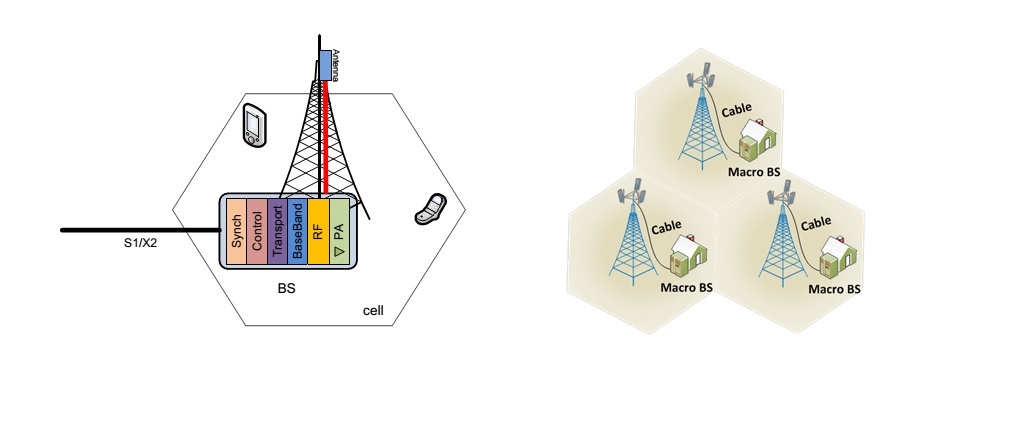
\includegraphics[scale=0.7]{./fig/c11}
  \caption{ساختار سنتی ایستگاه پایه \cite{checko2015cloud}}
  \label{fig:c11}
\end{figure}
هر ایستگاه پایه دو نوع پردازش انجام می‌دهد : پردازش
رادیویی که توسط واحد رادیویی \LTRfootnote{RRH} انجام می‌شود و شامل پردازش
دیجیتالی، فیلترینگ فرکانسی، تقویت توان و ....می‌باشد و
پردازش باند پایه که توسط واحد باند پایه \LTRfootnote{BBU} که همان واحد کنترل است \LTRfootnote{CU} انجام شده و از جمله
مهمترین وظایف آن می‌توان به کدینگ، مدولاسیون و
تبدیل فوریه ی سریع اشاره کرد. در ساختار جدیدی که
تحت عنوان \lr{C-RAN}  معرفی خواهیم نمود نحوه ی ارتباط
پردازشگرهای رادیویی و باند پایه متحول شده و در نتیجه
مزایایی برای شبکه حاصل خواهد شد.در ادامه، انواع ساختارها را بیان خواهد شد.
\subsubsection{ساختار سنتی ایستگاه پایه }

در ساختارهای سنتی ایستگاه پایه، پردازشهای رادیویی و باند پایه در
داخل ایستگاه پایه انجام ‌شد و مدول آنتن نیز در فاصله
ی چند متری از مدول رادیویی نصب شده و ارتباط آنها
توسط کابل کواکسیال برقرار میشد که همین امر سبب
افزایش تلفات در شبکه می‌باشد. این نوع ساختار در شکل
\ref{fig:c11} نشان داده شده است. همان گونه که مشاهده میکنید
ارتباط بین ایستگاه‌های پایه توسط ارتباط  $X_2$ و ارتباط بین
ایستگاه پایه و شبکه ی هسته توسط ارتباط $ S_1$ برقرار می
شود. این نوع ساختار در شبکه‌های \lr{1G} و \lr{2G} به کار گرفته
شده است 
\cite{checko2015cloud}.

%Figure \ref{fig:gull} shows a photograph of a gull.
\subsubsection{ ساختار ایستگاه پایه و واحد رادیویی}
\begin{figure}
  \centering
    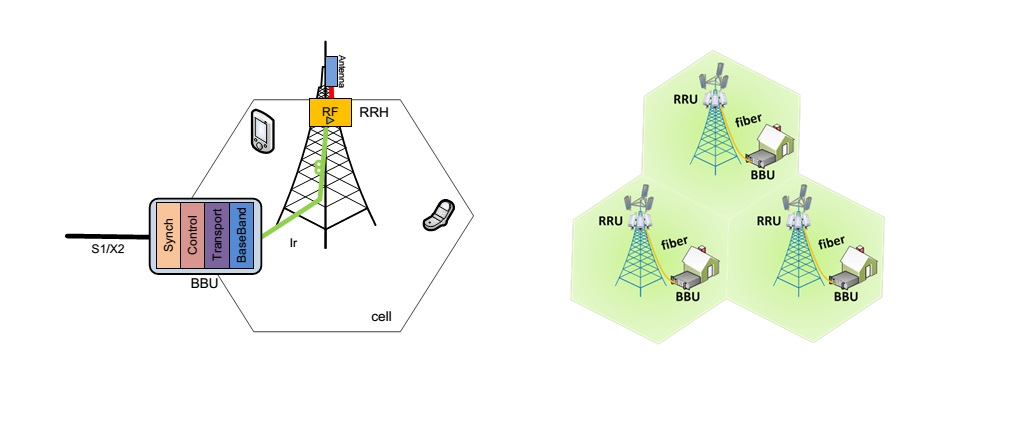
\includegraphics[scale=0.7]{./fig/c22}
  \caption{ ساختار ایستگاه پایه و واحد رادیویی \cite{checko2015cloud}}
  \label{fig:c22}
\end{figure}
در این ساختار واحد رادیویی و واحد پردازشی سیگنال، از هم
مجزا شده و واحد رادیویی که تحت عنوان \lr{RRH} یا \lr{RRU}
نیز شناخته می‌شود، توسط فیبر نوری به واحد باند پایه یا \lr{BBU} اتصال می‌یابد. همان طور که پیشتر بیان شد واحد رادیویی مسئولیت
انجام پردازشهای دیجیتالی از جمله تبدیل انالوگ به
دیجیتال، دیجیتال به انالوگ، تقویت توان و فیلترینگ رابر عهده دارد، که تفکیک وظایف واحد پردازشی و واحد
رادیویی در این ساختار در شکل \ref{fig:c22} قابل مشاهده است. این
نوع ساختار برای شبکه‌های نسل سوم معرفی شده و امروزه
نیز بیشتر ایستگاه‌های پایه از همین ساختار بهره میگیرند.
از جمله ویژگیهای بارز این ساختار امکان ایجاد فاصله
بین واحد رادیویی و پردازشی می‌باشد، که این فاصله به
دلیل تاخیر پردازشی و انتشاری نمیتواند از  $40$کیلومتر
فراتر رود. در این ساختار تجهیزات مرتبط با \lr{BBU} می
توانند به مکانی مناسبتر که قابل دسترس تر بوده و هزینه
ی اجاره و نگهداری کمتری را به اپراتورها تحمیل می
کنند منتقل شوند و واحدهای رادیویی نیز در در پشت بام
ساختمانها و مکانهای مرتفع نصب می‌شوند که این
خود سبب کاهش هزینه‌های خنک سازی ادوات موجود
می‌شود. نحوه ی ارتباط بین \lr{RRH} و \lr{BBU} مشابه ساختار
سنتی بوده و \lr{RRH}ها نیز توسط معماری زنجیروار باهم
در ارتباطند.
\begin{figure}
  \centering
    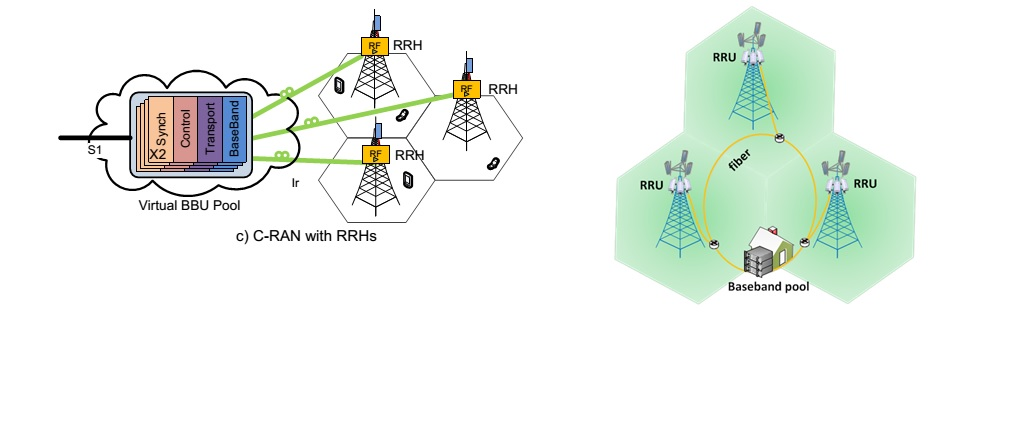
\includegraphics[scale=0.7]{./fig/c33}
  \caption{ساختار  \lr{C-RAN} \cite{checko2015cloud}}
  \label{fig:c33}
\end{figure}
\subsubsection{ساختار \lr{C-RAN}}
در ادامه ساختارهای شبکه دسترسی رادیویی ابری و ساختارهای بهبود یافته ی آن را معرفی می‌نماییم.
\begin{itemize}
\item \textbf{شبکه‌های دسترسی رادیویی ابری}


ایده اصلی \lr{C-RAN} جداسازی بخش رادیویی (\lr{RRH}) 
\LTRfootnote{Radio Remote Head}
 از واحد پردازشی باند پایه (\lr{BBU})
 \LTRfootnote{Baseband Unit}
  است.
از تجمیع \lr{BBU}ها بر روی سرور ابری، \lr{BBU-Pool} ایجاد می‌شود.
در این ساختار، در راستای بهینه سازی عملکرد \lr{BBU}
ها در مواجهه باایستگاه‌های پایه پر ترافیک و کم ترافیک،
 \lr{BBU}ها به صورت یک مجموعه ی واحد تحت عنوان 
\lr{BBU Pool}
 در آمده اند که این مجموعه بین چندین سلول 
 به اشتراک گزارده شده و مطابق شکل زیر مجازی سازی
می‌شود. 
در توضیح بیشتر این ساختار میتوان این گونه
عنوان کرد که \lr{BBU Pool} به عنوان یک خوشه ی مجازی
در نظر گرفته می‌شود که شامل پردازش گرهایی می‌باشد
که پردازش‌‌ باند پایه را انجام می‌دهند. ارتباط بین
  \lr{BBU}ها در ساختارهای فعلی به شکل  $X_2$ برقرار می‌شود
که در این ساختار ارتباط بین خوشه‌ها از فرم جدید $X_2$
تحت عنوان  $X_2 +$برقرار می‌شود.
\newline
در شکل \ref{fig:C-RAN} ساختار کلی شبکه‌ی  \lr{C-RAN} در سیستمهای
\lr{ LTE}
 نمایش داده شده است. همان طور که در شکل قابل
مشاهده می‌باشد ساختار کلی شبکه  \lr{C-RAN} به دو بخش
 \lr{backhaul} و \lr{fronthaul} تقسیم بندی شده‌است. بخش
 \lr{fronthaul}شبکه به مرحله ی اتصال سایتهای \lr{ RRH}به
 به \lr{BBU Pool} به اتصال \lr{backhaul} و بخش \lr{BBU Pool}
هسته ی شبکه ی سیار اطلاق می‌شود. همان گونه که قبلا
ذکر شد \lr{ RRH}ها در نزدیکی انتن نصب شده و از طریق
لینکهای انتقالی نوری با پهنای باند وسیع و تاخیر کم به
پردازشگرهای قوی در \lr{BBU} متصل می‌شوند. توسط این
لینکهای انتقالی است که سیگنالهای دیجیتالی باند
پایه از نوع \lr{IQ} بین \lr{RRH} و \lr{BBU} انتقال می‌یابند \cite{checko2015cloud}.
\begin{figure}
  \centering
    \includegraphics[width=\textwidth]{./fig/CRAN}
  \caption{ساختار شبکه‌ی \lr{C-RAN} \cite{checko2015cloud}}
  \label{fig:C-RAN}
\end{figure}
\item \textbf{شبکه‌های دسترسی رادیویی ابری نامتجانس (\lr{H-CRAN})}


برای غلبه بر چالشهای شبکه‌های \lr{C-RAN} با محدودیتهای \lr{fronthaul}، شبکه‌های دسترسی ابری نامتجانس (\lr{H-CRAN}) معرفی می‌شود\cite{ fogComputing, heterogeneous, fogEdge}.
\begin{figure}
  \centering
    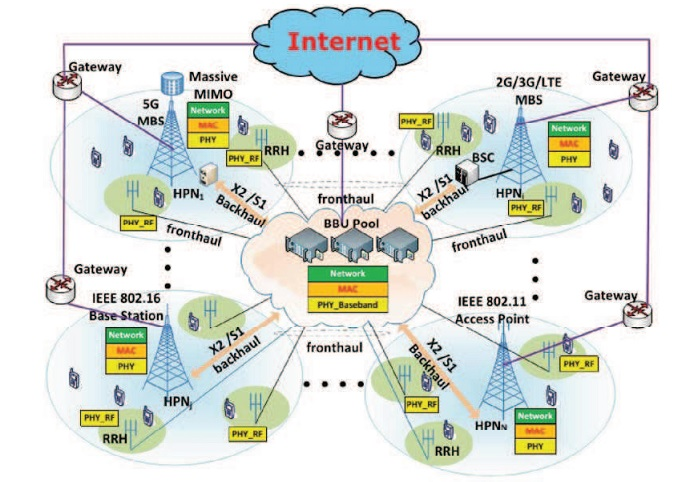
\includegraphics[scale = 0.8]{./fig/hc}
  \caption{ ساختار شبکه‌های دسترسی ابری نامتحانس \cite{heterogeneous}  }
  \label{fig:hc}
\end{figure}

صفحه‌ی کاربر و صفحه ی کنترلگر در چنین شبکه‌هایی از هم مجزا می‌باشند. 
در این شبکه‌ها، نودهای توان بالا   \LTRfootnote{High Power Node}\lr{HPN}، عمدتا برای فراهم کردن پوشش بدون درز و اجرای عملکرد صفحه کنترل می‌باشد. در حالی که \lr{RRH}ها برای فراهم نمودن سرعت بالای نرخ داده برای انتقال بسته در ترافیک قرار گرفته اند. \lr{HPN}ها از طریق لینکهای \lr{backhaul}  به \lr{BBU Pool} متصلند ( برای هماهنگ کردن تداخل ).\newline
ساختار این شبکه شبیه به ساختار \lr{C-RAN} می‌باشد. همانطور که در شکل \eqref{fig:hc} نشان داده شده است، تعداد زیادی \lr{RRH}، همراه با انرژی مصرفی کم در ساختار \lr{H-CRAN}، با یکدیگر در \lr{BBU Pool} مرکزی، همکاری می‌کنند تا گین مشترک بالایی بدست آورند. تنها‌، فرکانس رادیویی جلو، (\lr{RF}) و عملکردهای پردازشی  ساده، در \lr{RRH}، صورت میگیرد، در حالی که پردازشهای مهم دیگر، در \lr{BBU Pool} انجام می‌گیرد. همچنین تنها بخشی از عملکردها در لایه ی \lr{PHY} در \lr{RRH} به مشارکت می‌انجامد که این مدل در شکل \eqref{fig:hc} نشان داده شده است.\newline
اگرچه، برخلاف \lr{C-RAN}،
\lr{BBU Pool} در \lr{H-CRAN}، به \lr{HPN}ها متصلند که این، برای کاهش تداخل متقابل بین \lr{RRH}ها و \lr{HPN}ها از طریق محاسبات ابری متمرکز براساس تکنیکهای پردازشی مشترک می‌باشد. همچنین، داده و واسط کنترل، بین \lr{BBU Pool} و \lr{HPN}های $S_1$ و $X_2$ شناخته شده اند که تعریف آنها بر اساس تعریف استاندارد \lr{3G} ایجاد شده است.\newline
همانطور که سرویسهای صدا، میتوانند به صورت بهینه در طول مد سوییچ بسته در \lr{4G} فراهم گردند، \lr{H-CRAN} میتواند به طور همزمان سرویس صدا و داده را پشتیبانی کند. سرویس صدا مرجح به اداره از طریق \lr{HPN}ها می‌باشد، در حالی که ترافیک بسته ی پر داده، بیشتر توسط \lr{RRH} اداره می‌گردد. 
در مقایسه با ساختار \lr{C-RAN}، ساختار \lr{H-CRAN} نیازهای \lr{fronthaul} را بوسیله ی مشارکت \lr{HPN}ها برطرف می‌سازد. با توجه به حضور \lr{HPN}ها، سیگنالهای کنترلی و سمبلهای داده در \lr{H-CRAN} جدا از هم می‌باشند. تمام کنترل کننده‌های سیگنال و سیستمهایی که اطلاعات را ارسال می‌نمایند، توسط \lr{HPN}ها به \lr{UE}، منتقل می‌گردد که منجر به سادگی در ظرفیت و در محدودیت تاخیر زمان در لینکهای \lr{fronthaul } بین \lr{RRH}ها و \lr{BBU Pool}  می‌گردد و منجر به صرفه‌جویی در مصرف انرژی می‌گردد. همچنین، برخی از ترافیکهای شدید و ناگهانی \LTRfootnote{Burst Traffic} و یا سرویس پیام همراه با مقدار داده‌ی کم، می‌تواند به صورت بهینه توسط \lr{HPN}ها پشتیبانی گردد. مکانیزم کنترل بین ارتباط داشتن و نبود ارتباط، توسط \lr{H-CRAN} پشتیبانی می‌گردد که منجر به حفظ کردن مقدار قابل توجهی \lr{Overhead} در رادیو بوسیله ی مکانیزم ارتباط جهت دار خالص می‌گردد. در \lr{RRH}، تکنولوژیهای مختلف انتقال در لایه ی \lr{PHY}، قابل استفاده برای بهبود نرخ انتقال (همانند موج میلیمتری و نور مرئی) می‌گردد. در \lr{HPN}ها، \lr{MIMO}\LTRfootnote{Multiple Input Multiple Output}، یکی از راه‌های افزایش پوشش در بهبود ظرفیت می‌باشد.

\item \textbf{ساختار دسترسی رادیویی مهی}


برای حل کردن مشکلات \lr{H-CRAN} و \lr{C-RAN}، نیاز به معرفی ساختار جدید دیگری می‌باشیم که آن را \lr{F-RAN} می‌نامیم.
\lr{F-RAN} 
تمام ویژگیهای مثبت محاسبات ابری و شبکه‌های نامتجانس و محاسبات مهی را همزمان در بر می‌گیرد.
محاسبات مهی، اصطلاحی برای جایگزین کردن محاسبات ابری است که مقدار قابل توجهی از ذخیره سازی، ارتباطات، کنترل کردن، اندازه گیری و مدیریت را در لبه ی شبکه انجام می‌دهد (نه در کانال و ابر مرکزی) \cite{fogComputing, fogEdge}.
 سیستمهای \lr{F-RAN} تحولی از سیستمهای \lr{C-RAN} می‌باشد که برخی از ارتباطات توزیع شده و عملکردهای ذخیره سازی در منطق لایه ی مه قرار دارد. همچنین چهار نوع ارتباطات ابری تعریف شده است.
  \begin{figure}[H]
  \centering
    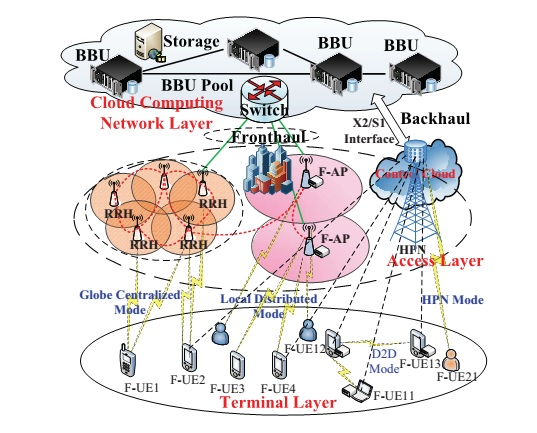
\includegraphics[scale =0.7]{./fig/fr}
  \caption{ مدل سیستم \lr{F-RAN} \cite{fogComputing} }
  \label{fig:fr}
\end{figure}
 \begin{itemize}
 \item
 ابر ذخیره‌گر و ارتباطات مرکزی جامع :
 که همانند ابر مرکزی \lr{C-RAN} می‌باشد.
 \item
 ابر کنترل‌گر مرکزی :که برای تکمیل عملکردهای کنترلی می‌باشد و در \lr{HPN}ها قرار دارد.
 \item
 ابر ارتباطات منطقی توزیع شده که در برنامه‌های محاسبات مهی و ابزارهای این محاسبات قرار دارد.
 \item
  ابر ذخیره گر منطق توزیع شده:
  که همانند قبل در \lr{F-RAN} قرار دارد.
 \end{itemize}
 در این ساختار، برای کاهش تاخیر ناشی از انتقال داده‌ها به ابر مرکزی، ساختارهای \lr{RRH} را دارای حافظه قرار می‌دهیم که برای ارتباطات محلی، به جای اینکه پردازشها در \lr{BBU Pool} صورت بگیرد، بدون نیاز به انتقال به ابر مرکزی، درون \lr{RRH}ها انجام پذیرد. 
\end{itemize}
\subsection{\lr{xRAN}}
\lr{xRAN}
در سال ۲۰۱۶ با هدف استانداردسازی یک جایگزین انعطاف پذیر و باز برای \lr{RAN}
مبتنی بر سخت افزار سنتی بدست آمده‌است.
 در این ساختار، سه حوزه ی مهم مورد بررسی قرار گرفته است.
اولین حوزه ی مورد بررسی، جداسازی بخش
صفحه ی کنترل
 \LTRfootnote{control plane} از 
 صفحه‌ی کاربر
\LTRfootnote{user plane}
می‌باشد. حوزه ی دوم،
ساختن یک پشته نرم‌افزاری \lr{eNodeB} مدولار که از سخت افزار \lr{COTS} استفاده می‌کند، می‌باشد.
حوزه ی سوم مورد بررسی، انتشار رابطهای باز شمال و جنوب است\cite{xran}.
در ادامه این سه حوزه به طور دقیق تر مورد بررسی قرار میگیرد\cite{xran1}.

\begin{itemize}
\item \textbf{ جداسازی بخش صفحه ی کنترل از 
صفحه ی کاربر}:
این انتقال صفحه ی کنترل، که قبلاً کاملاً به دستگاه‌های سخت افزاری \lr{RAN} متصل بود، به دستگاه‌های محاسباتی در دسترس امکان می‌دهد \lr{RAN} بتواند به عنوان یک استخر منطقی از ظرفیت، با کارایی بیشتری کار کند.
نرم‌افزار \lr{eNodeB} از سخت افزار خاص فروشنده جدا می‌شود و الهام بخش نوآوری در هر دو نرم‌افزار و سخت افزار به صورت مشارکتی اما به طور مستقل است.
برنامه نویسی و کنترل زمان واقعی بی سابقه در زیرساختهای \lr{RAN} به دست آمده است، که به راحتی از برنامه‌های کاربردی تلفن همراه و خدمات تجاری پشتیبانی می‌کند.
\item \textbf{ساختن یک پشته نرم‌افزاری \lr{eNodeB} مدولار}:
رویکرد \lr{xRAN} به خوبی با طرحهای مجازی سازی عملکرد شبکه حامل \lr{(NFV)} مطابقت دارد، و همچنین منجر به کنترل عملکرد ترافیک با کارایی بالا، مدیریت تداخل و کنترل منابع رادیویی روی سیستم عاملهای استاندارد \lr{x86} می‌شود.
\item \textbf{انتشار رابطهای باز شمال و جنوب}: 
رابطهای استاندارد و باز قابلیت پشتیبانی از فروشنده‌های متعدد همکاری اثبات شده دارند. 
\lr{xRAN.org}
و اعضای آن به تصویب رساندن این رابطها از طریق فرآیندهای استاندارد منجر به در دسترس قرار دادن معماری \lr{xRAN} و پشتیبانی مورد نیاز می‌شوند.

\end{itemize}
در ادامه مزایای ساختار xRAN را بیان می‌نماییم.

\textbf{مزایای ساختار xRAN}
%\subsubsection{مزایای ساختار \lr{xRAN}}
\begin{itemize}
\item 
جداسازی بخش صفحه ی کنترل از 
صفحه ی کاربر 
منجر به 
برنامه ریزی زمان واقعی بی سابقه و کنترل در زیرساخت \lr{RAN} می‌شود که به راحتی برنامه‌های کاربردی تلفن همراه و خدمات تجاری را پشتیبانی می‌کند.
\item
 یک پشته
 \lr{eNB} 
 مدولار مبتنی بر نرم‌افزار، منجر به امکان قرارگیری انعطاف پذیر توابع \lr{eNB} و کنترل ترکیبی آن با یک برنامه ریز امکان پذیر می‌شود تا بتواند زمان تاخیر متغیر در \lr{fronthaul} را کنترل کند.
\item
رابط‌های مرزی جنوبی استاندارد، پیاده سازی شبکه با خرید سیستم از چندین شرکت متفاوت را امکان پذیر می‌سازد و رابطهای شمال مرزی، برش کامل شبکه برای بهینه سازی \lr{QoE} \LTRfootnote{Quality of Experience} کاربر را فراهم می‌کند.
رابطهای \lr{xRAN} به خوبی با لبه ابر حامل هماهنگ هستند و اجازه می‌دهد تا محاسبه و ذخیره سازی منابع در شبکه تلفن همراه 
به صورت دینامیکی مدیریت شود.
\item 
این ساختار هزینه‌ی رشد ظرفیت دسترسی رادیویی و هزینه‌ی بهره برداری را کاهش می‌دهد.
\end{itemize}
\subsection{vRAN}
vRAN 
یا شبکه‌های دسترسی رادیویی مجازی
گونه‌ی دیگری از شبکه‌های رادیویی دسترسی می‌باشند که منجر به افزایش هوشمندانه ظرفیت، کاهش چشمگیر هزینه‌ها می‌شود. همچنین قابلیت انعطاف پذیری و مقیاس پذیری پویا را فراهم می‌کند که برای پشتیبانی از خدمات و برنامه‌های آینده ضروری خواهد بود.
معماری vRAN با اجرای توابع باند پایه مجازی بر روی سخت افزار سرور کالا، بر اساس اصول مجازی سازی توابع شبکه (NFV)، فراتر از آخرین شبکه‌ی  متمرکز رادیویی (C-RAN) است.
معماری C-RAN می‌تواند با ایجاد امکان تجمع منابع پردازش باند پایه، که می‌تواند به صورت پویا به سایتهای مختلف سلول و فن‌آوریهای رادیویی اختصاص یابد، گامی فراتر رود.
به اشتراک گذاری منابع باند پایه از طیف موجود با کارآیی بیشتری استفاده می‌کند و قابلیت اطمینان سرویس را بهبود می‌بخشد.
همچنین پشتیبانی از ویژگی‌های LTE-Advanced و استقرار سلولهای کوچک  می‌تواند ظرفیت را در مناطق پرجمعیت و نقاط پرتردد افزایش دهد.
اما تمرکز باند متمرکز (BBU-Pool) به اندازه کافی پیش نمی‌رود.
برای دستیابی به پتانسیل کامل صرفه‌جویی در هزینه، مقیاس گزاری ظرفیت پویا، کیفیت بالاتر و ارائه سریع سرویسهای جدید، می‌بایست از یک معماری RAN مجازی (vRAN) استفاده کنند. در مدل vRAN،
BBU 
مجازی شده است.
vBBU
که همان واحدهای باند پایه‌ی مجازی هستند، در چندین سیستم عامل NFV در سخت افزار استاندارد x86 مستقر شده و در مراکز داده متمرکز تلفیق می‌شوند، در حالی که واحدهای رادیویی از راه دور (RRH) در سایتهای سلول در لبه باقی می‌مانند.
vRAN 
از سخت افزار استاندارد سرور استفاده می‌کند که به طور مقرون به صرفه پردازش، حافظه و منابع ورودی و خروجی را با تقاضای خود، درخواست می‌کند و ظرفیت RAN را با هوش مصنوعی تغییر داده تا کیفیت و قابلیت اطمینان خدمات را به طور قابل توجهی بهبود بخشد.
بسته به نحوه تقسیم عملکردهای eNodeB، معماری vRAN همچنین امکان انتقال اترنت و IP را فراهم می‌کند، که به ارائه‌دهندگان خدمات گزینه‌های مقرون به صرفه‌تری برای انتقال fronthaul می‌دهد \cite{vran}.
\begin{figure}%[H]
	\centering
	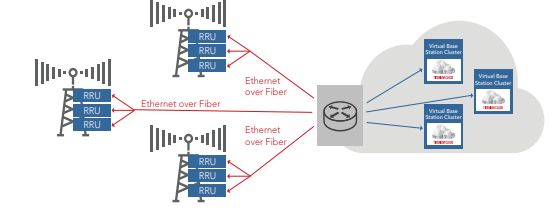
\includegraphics[width=0.8\textwidth]{./fig/vran}
	\caption{ساختار شبکه ی \lr{vRAN} \cite{vran}}
	\label{fig:vran}
\end{figure}


\subsection{مقدمه ای بر ORAN}
شبکه دسترسی رادیویی باز از ترکیب C-RAN و xRAN و در برخی جاها از ترکیب C-RAN و vRAN بدست آمده است.
معماری \lr{ORAN} برای ایجاد زیرساختهای \lr{RAN} نسل بعدی طراحی شده است.
معماری \lr{ORAN} با تکیه بر اصول هوشمندی و باز بودن، پایه و اساس ساخت \lr{RAN} مجازی بر روی سخت افزار آزاد، با کنترل رادیویی ایجاد شده توسط هوش مصنوعی است که توسط اپراتورهای سراسر جهان پیش بینی شده است.
این معماری بر روی رابطهای استاندارد و تعریف شده ای بنا شده است تا یک زنجیره اکوسیستم با قابلیت باز ایجاد کند که دارای پشتیبانی کامل از استانداردهای تبلیغ شده توسط \lr{3GPP} و سایر سازمانهای استاندارد صنعت فراهم شود.
\begin{figure}%[H]
  \centering
    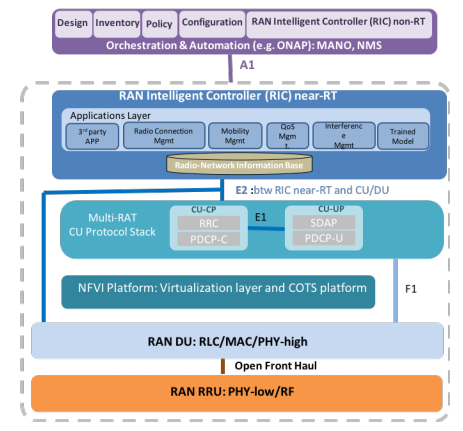
\includegraphics[width=0.8\textwidth]{./fig/oran1}
  \caption{ساختار شبکه ی \lr{ORAN} \cite{oranWP}}
  \label{fig:ORAN}
\end{figure}
اتحاد \lr{ORAN} در جستجوی چشم انداز باز بودن و هوشمندی برای شبکه‌های بی سیم نسل بعدی و فراتر از آن است\cite{oranWP}.
این دو ویژگی مهم در ادامه مورد بررسی قرار گرفته شده است.
\begin{itemize}
\item \textbf{باز بودن}:
ایجاد یک \lr{RAN} مقرون به صرفه نیاز به باز بودن ارتباط‌ها دارد.
رابطهای باز برای فعال کردن فروشندگان و اپراتورهای کوچکتر به سرعت میتوانند خدمات خود را معرفی کنند و یا اپراتورها را قادر می‌سازد تا شبکه را متناسب با نیازهای منحصر به فرد خود تنظیم کنند.
رابطهای باز همچنین استقرار چند سازنده ای را قادر می‌سازد و اکوسیستم تأمین کننده رقابتی تر و پر جنب و جوش بیشتری را ایجاد می‌کند.
 همچنین نرم‌افزارهای منبع باز و طرحهای مرجع سخت افزار باعث نوآوری سریعتر و دموکراتیک تر می‌شود.
 \item \textbf{هوشمندی}
 شبکه‌ها با ظهور برنامه 5G پیچیده تر و متراکم تر شده و خواستار برنامه‌های غنی تر می‌شوند.
 برای کاستن این پیچیدگی نمیتوان از ابزارهای سنتی انسانی  برای استقرار، بهینه سازی و بهره برداری از شبکه استفاده کرد.
 در نتیجه، شبکه‌ها باید خود متحرک شوندتا بتوانند از فن آوریهای جدید مبتنی بر یادگیری برای خودکارسازی عملکرد شبکه‌های عملیاتی و کاهش \lr{OPEX} استفاده کنند.
 اتحاد \lr{ORAN} تلاش خواهد کرد تا از تکنیکهای یادگیری عمیق در حال ظهور استفاده کند تا بتواند هر لایه از معماری \lr{RAN}  را به طور هوشمند پیاده سازی کند.
 پیاده سای هوشمند هم در مولفه‌ها و هم در سطح شبکه اعمال می‌گردد و منجر به تخصیص دینامیکی منابع رادیویی و بهینه سازی بازدهی شبکه می‌گردد.
 همراه با رابطهای باز \lr{ORAN}، اتوماسیون حلقه بسته بهینه شده با هوش مصنوعی دست یافتنی است و دوره جدیدی را برای عملیات شبکه امکان پذیر می‌کند.
\end{itemize}
در ادامه ویژگی های این ساختار را بررسی می‌نماییم.
\begin{itemize}
\item \textbf{روشهای هوش مصنوعی \lr{AI}
 \LTRfootnote{Artificial Intelligent}
  منجر به هوشمندسازی بخش رادیویی با استفاده از نرم‌افزار تعریف شده \LTRfootnote{Software Defined} 
  می‌شود:}
   مفهوم 
  \lr{SDN}
  \LTRfootnote{software defined network}
  که مبنی بر جداسازی 
   بخش صفحه ی کنترل \lr{CP} از
   صفحه‌ی کاربر 
\lr{UP}
می‌باشد، در ساختار 
\lr{ORAN}
مورد بررسی قرار می‌گیرد.
این جداسازی منجر به بهبود 
\lr{RRM}
برای استفاده از زمان غیر واقعی و زمان نزدیک به واقعی در کنترلگر هوشمند شبکه ی دسترسی رادیویی \LTRfootnote{RAN Intelligent Controller} \lr{RIC} 
با استفاده از رابط‌های 
\lr{A1}
و
\lr{E2}
 می‌‌گردد.
همچنین 
منجر به جداسازی 
 \lr{CU}
 از 
 \lr{CP/UP}
 می‌شود
 که از طریق رابط \lr{E1} در \lr{3GPP } توسعه می‌یابد.
\item \textbf{مجازی سازی بخش \lr{RAN}}:
 ابری سازی RAN یکی از اصول مهم ساختار 
 \lr{ORAN}
  می‌باشد.
 اپراتورها برای پشتیبانی از شکافهای مختلف در شبکه، الزامات NFVI/VIM را برای تقویت سیستم عامل مجازی ارائه می‌دهند.
 به عنوان مثال: لایه ی بالا بین PDCP و RLC تقسیم می‌شود و لایه ی پایین در PHY تقسیم می‌شود.
\item \textbf{رابطهای باز}:
معماری مرجع ORAN بر روی مجموعه ای از رابطهای کلیدی بین چندین جزء جدا شده ی RAN ساخته شده است.
اینها شامل رابطهای \lr{3GPP} پیشرفته 
(
\lr{F1}،
\lr{W1}،
\lr{E1}،
\lr{X2}،
\lr{Xn}
)
 برای قابلیت همکاری بین چندین شرکت مختلف تولید کننده است.
رابطهای مشخص شده \lr{ORAN Alliance} شامل یک رابط fronthaul باز بین DU و RRU، رابط \lr{E2} و یک رابط \lr{A1} بین لایه 
Orchestration/NMS 
است که شامل عملکرد
 غیر واقعی زمانی \LTRfootnote{non real time RIC} و عملکرد eNB / gNB حاوی عملکرد RIC نزدیک به زمان واقعی 
\LTRfootnote{near-real time RIC} 
است.
\item \textbf{سخت افزار جعبه سفید}:
برای بهره مندی کامل از مقیاسی از اقتصاد ارائه شده توسط یک رویکرد  محاسباتی باز، \lr{O-RAN Alliance } 
طرحهای مرجع 
سخت افزاری و ایستگاه پایه به صورت جعبه سفید با کارایی بالا را مشخص می‌کند. 
سیستم عاملهای مرجع از یک رویکرد جدا شده پشتیبانی میکنند و نقشه‌های مفصلی را برای معماری سخت افزار و نرم‌افزار ارائه می‌دهند تا هم BBU و RRU را فعال کنند. 
\item \textbf{نرم‌افزار منبع باز}:
اتحادیه ORAN ارزش انجمنهایی که منابع باز ارا‌ئه می‌دهند را درک کرده   
 و از آنها پشتیبانی می‌کند.
 بسیاری از مؤلفه‌های معماری ORAN به صورت منبع باز از طریق جوامع موجود تحویل داده می‌شود.
 این مؤلفه‌ها عبارتند از: کنترلر هوشمند RAN، پشته پروتکل، پردازش لایه PHY و بستر مجازی سازی.
  چارچوب نرم‌افزار منبع باز ORAN نه تنها رابطهای 
(
\lr{F1}،
\lr{W1}،
\lr{E1}،
\lr{E2}،
\lr{X2}،
\lr{Xn}
)
  را پیاده سازی می‌کند، بلکه انتظار دارد که طراحی مرجع را برای نسل بعدی RRM با هوش جاسازی شده ارائه دهد تا RIC را امکان پذیر کند.
\end{itemize}

\lr{ORAN}،
 المانهای شبکه ی دسترسی رادیویی را مجازی می‌کند، آنها را جدا کرده و رابطهای باز مناسب را 
برای اتصال این عناصر
تعیین می‌کند. همچنین، 
\lr{ORAN}
از روشهای یادگیری ماشین برای هوشمندسازی لایه‌های 
\lr{RAN}
 استفاده می‌نماید. 
 در ساختار نوآورانه ی 
 \lr{ORAN}
 نرم‌افزار قابل برنامه ریزی 
 \lr{RAN}
 از سخت افزار جدا می‌شود.
  یکی از مهم ترین خصوصیات
  \lr{ORAN}
  رابط کاربری باز است که به اپراتورهای موبایل این قابلیت را می‌دهد تا بتوانند سرویسهای مورد نیاز خود را تعریف نمایند.

در ساختار
\lr{ORAN}،
واحد توزیع شده \lr{DU}،
نود منطقی می‌باشد که شامل لایه‌های 
\lr{RLC}
،
\lr{MAC}،
و
\lr{High-PHY}
است.
علاوه بر این، واحد مرکزی 
\lr{CU}
نود منطقی است که شامل لایه‌های 
\lr{RRC}،
\lr{SDAP} 
و 
\lr{PDCP}
می‌باشد.
نود منطقی واحد رادیویی
\lr{RU}
نیز، شامل لایه‌ی 
\lr{LOW-PHY}
و بخش پردازش رادیویی می‌باشد.
\lr{ORAN}
،
رابطهایی از جمله رابط 
\lr{fronthaul}
باز را شامل می‌شود که بخش \lr{DU} را به \lr{RU} متصل می‌نماید
(رابط 
\lr{E2}). 
همچنین
 رابط \lr{A1}
 بین لایه ی 
  \lr{orchestration/NMS}
  که شامل 
  تابع غیر واقعی زمان است و 
  \lr{eNB/qNB}
  که شامل تابع نزدیک به زمان است. 


  با افزایش ترافیک تلفن همراه، شبکه‌های تلفن همراه و تجهیزاتی که آنها را اجرا می‌کند باید نرم‌افزاری تر، مجازی، انعطاف پذیر، هوشمند و کارآمدتر شوند.
اتحادیه ی ORAN متعهد است در حال تکامل شبکه‌های دسترسی رادیویی باشد که باعث می‌شود آنها نسبت به نسلهای قبل بازتر و باهوش تر شوند.
تجزیه و تحلیل در زمان واقعی که توسط سیستمهای یادگیری ماشین تعبیه شده است و ماژولهای پایانی هوش مصنوعی را هدایت می‌کند، باعث تقویت هوش شبکه ‌‌شود.
عناصر شبکه مجازی با رابطهای باز و استاندارد، جنبه‌های اصلی طرحهای مرجع توسعه یافته توسط اتحادیه ی ORAN خواهد بود.
فن آوریهای موجود از عناصر شبکه منبع باز و جعبه سفید، نرم‌افزار و اجزای سخت افزاری مهم این طرحهای مرجع خواهد بود.

\subsubsection{ساختار ORAN}
O-RAN Alliance~\footnote{https://www.o-ran.org} اخیراً طراحی یک معماری جدید
 RAN را برای تحقق بخشیدن به چشم انداز تبدیل RAN به باز، هوشمند، مجازی سازی شده و کاملاً تعامل پذیر راه اندازی کرده است. توانمندسازی چنین ویژگی‌هایی برای توانمندسازی نسل بعدی شبکه‌های سلولی بی‌سیم برای پاسخگویی به نیازهای خدمات متنوع به روشی مقرون‌به‌صرفه حیاتی است. مفهوم ORAN مزایای مفاهیم C-RAN و vRAN را ترکیب و تکامل می دهد. ORAN با تکیه بر تلاش های قبلی برای ابری سازی و متمرکز سازی واحدهای باند پایه معرفی شده توسط C-RAN و جداسازی نرم افزار از سخت افزار فعال شده توسط vRAN، می آید تا با تعریف رابط های باز استاندارد بین، مشکلات قفل فروشنده و پیاده سازی اختصاصی را حل کند. اجزای RAN گشودگی ارائه شده توسط ORAN اجازه می دهد تا یک اکوسیستم زنجیره تامین با چند فروشنده را تقویت کند. علاوه بر باز بودن، ORAN هوش شبکه را از طریق ادغام AI/ML در اجزای RAN ارتقا می دهد.
 
 \begin{figure}%[htbp]
 	\centering
 	%\resizebox{\linewidth}{!}{
 	\resizebox{7.5cm}{!}{
 		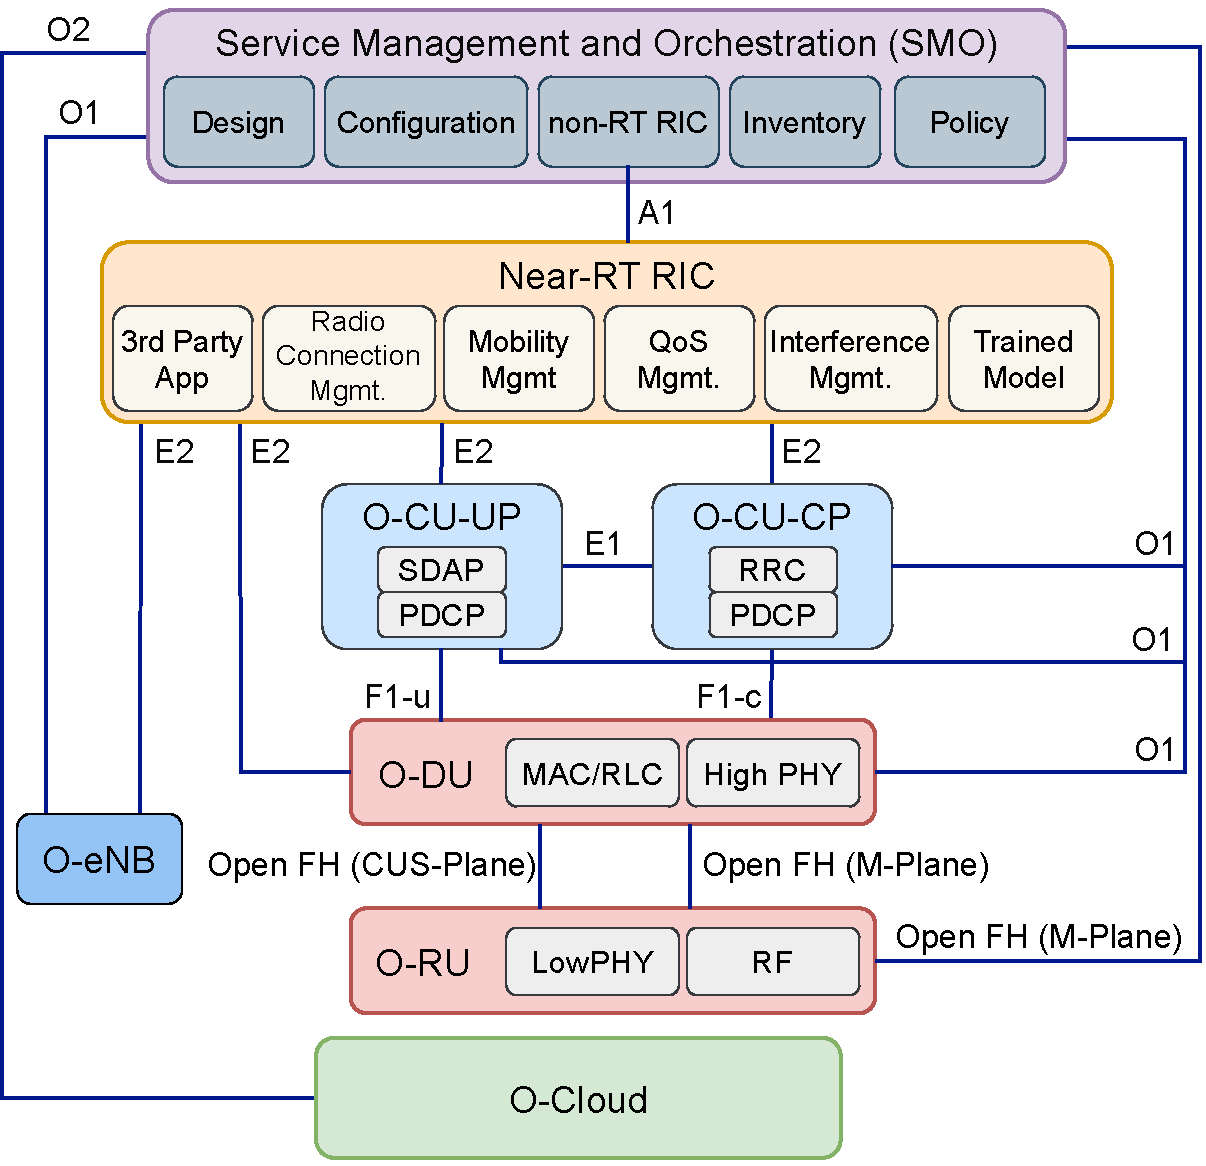
\includegraphics{img/oran_last_new.pdf}
 	}
 	\caption{ساختار ORAN}
 	\label{fig:g11}
 \end{figure}

ORAN با تقسیم RAN خود به چندین مؤلفه کاربردی، یک RAN هوشمند و همه کاره ایجاد می کند.
برخلاف معماری C-RAN که دارای دو واحد RAN است، یعنی واحد رادیویی و باند پایه، O-RAN شامل سه واحد است: واحد رادیویی (O-RU)، واحد توزیع شده (O-DU) و واحد مرکزی (O-CU).
تصویر \ref{fig:g11} معماری ORAN را نشان می دهد.
معماری منطقی ORAN شامل سمت رادیویی، سمت مدیریتی و سمت ابری است.
\begin{itemize}
	\item بخش رادیویی:
	در سمت رادیویی از لایه‌های منطقی مختلف، از جمله 
	O-RU، O-DU، O-CU  
	و
	کنترل‌کننده هوشمند رادیویی نزدیک به زمان واقعی (near RT RIC) تشکیل شده است.
O-RU شامل لایه فرکانس رادیویی (RF) و لایه فیزیکی پایین (PHY) است، در حالی که O-DU عملکردهای لایه های PHY بالا، کنترل دسترسی متوسط (MAC) و کنترل پیوند رادیویی (RLC) را ارائه می دهد.

فرانتهال باز (Open-FH) رابط بین O-RU و O-DU است. رابط Open-FH شامل یک صفحه هماهنگ سازی کاربر کنترل (CUS-plane) و یک صفحه مدیریت (M-plane) است. رابط Open-FH M-plane O-RU را برای قابلیت های خطا، پیکربندی، حسابداری، عملکرد و امنیت (FCAPS) به مدیریت خدمات و هماهنگ سازی (SMO) متصل می کند.	

O-CU به دو گره منطقی صفحه کاربر (O-CU-UP) و صفحه کنترل (O-CU-CP) تقسیم می شود. O-CU-UP شامل پروتکل تطبیق داده های سرویس (SDAP) است که کیفیت خدمات حامل های رادیویی را مدیریت می کند. و بخش صفحه کاربر از پروتکل همگرایی داده های بسته (PDCP) که عملکردهای انتقال داده، تکرار بسته ها، رمزگذاری و حفاظت از یکپارچگی و غیره را فراهم می کند.

O-CU-CP میزبان لایه کنترل منابع رادیویی (RRC) است که چرخه عمر اتصال و صفحه کنترل پروتکل PDCP را کنترل می کند.

\item بخش مدیریتی:
سمت مدیریت شامل چارچوب SMO است. در SMO، RIC غیر RT نقش مهمی دارد \cite{ORANArch}.
RIC غیر RT رویدادها و مدیریت منابع را با زمان پردازش حداقل 1 ثانیه مدیریت می کند. مدیریت منابع شامل
بهینه سازی در RAN، استفاده از سیاست ها و مدل های ML برای RIC های نزدیک به RT برای افزایش عملکرد سیستم.
علاوه بر این، مدیریت چرخه حیات را برای اجزای شبکه فراهم می کند. علاوه بر این، پیکربندی و سایر جنبه های حیاتی یک شبکه را انجام می دهد.
\item بخش ابری:
این یک پلت فرم محاسبات ابری به نام O-Cloud را نشان می دهد که می تواند میزبان اجزای معماری O-RAN باشد که در شکل \ref{fig:g12} نشان داده شده است.
پلتفرم O-Cloud شامل زیرساخت سخت افزاری و فناوری های مجازی سازی است که برای فعال کردن نرم افزار O-RAN و جداسازی سخت افزار \cite{ORANSecOcloud} لازم است. زیرساخت سخت افزار مجموعه ای از سرورهای تجاری خارج از قفسه (COTS) است که منابع مدیریت محاسبات، ذخیره سازی، شبکه و سخت افزار را فراهم می کند.
توابع شبکه RAN را می توان به ترتیب به صورت توابع شبکه مجازی شده (VNF) یا توابع شبکه بومی ابری (CNF) در حال اجرا بر روی ماشین های مجازی (VM) یا کانتینرها مستقر کرد. لایه مجازی سازی پلت فرم O-Cloud شامل اجزای نرم افزاری پشتیبانی کننده (مانند سیستم عامل ها، هایپروایزرها و موتورهای کانتینری) برای اجرای VNF و CNF های RAN است.
O-Cloud همچنین از شتاب دهنده های سخت افزاری و یک لایه انتزاعی شتاب (AAL) پشتیبانی می کند که مجموعه ای از API های باز را برای بارگذاری عملکردهای شبکه O-RAN با شتاب سخت افزاری تعریف می کند.
SMO از طریق رابط $\text{O}2$ به O-Cloud برای ارائه منابع پلت فرم و قابلیت های مدیریت حجم کار \cite{ORANArch} متصل می شود.
\begin{figure}
	\centering
	%\resizebox{\linewidth}{!}{
	\resizebox{7.5cm}{!}{
		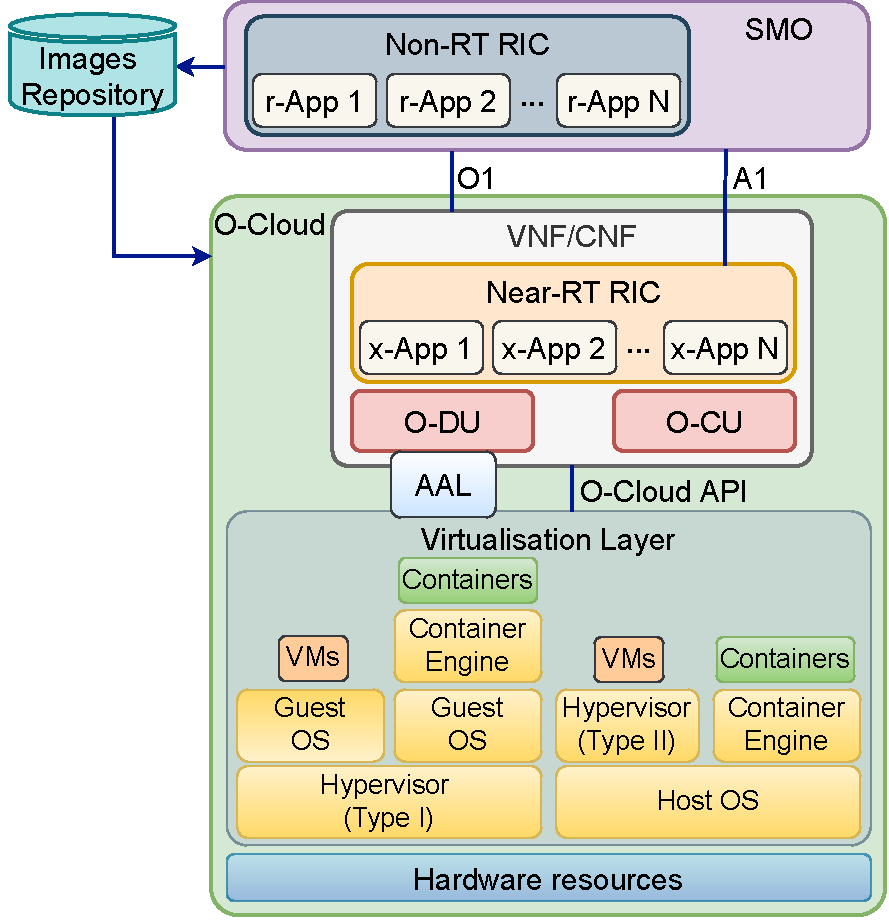
\includegraphics{img/ocloud_new.pdf}
	}
	\caption{ ساختار O-Cloud}
	\label{fig:g12}
\end{figure}

\end{itemize}

\subsubsection{آسیب پذیری ها و تهدیدها در معماری ORAN}
در این بخش هدف، صحبت در مورد آسیب پذیری‌ها و تهدیدها در معماری ORAN می‌باشد.

باز بودن و تفکیک معماری ORAN راه را برای یک وضعیت امنیتی تقویت شده برای شبکه های تلفن همراه آینده هموار می کند و انطباق با استانداردهای امنیتی را تسهیل می کند و چابکی امنیتی، سازگاری و انعطاف پذیری را تقویت می کند. با این حال، با این مزایا، پتانسیل افزایش سطح حمله ارائه شده توسط مؤلفه‌ها و رابط‌های جدید معماری ORAN \cite{ORANSec} به وجود می‌آید. در ادامه این بخش، آسیب‌پذیری‌ها و تهدیدات اصلی علیه سیستم ORAN را با در نظر گرفتن نه تنها مواردی که توسط فن‌آوری‌های جدید و اصول طراحی معماری ORAN به ارمغان می‌آورند، بلکه همچنین مسائل رایج امنیتی \lr{5G} RAN را مورد بحث قرار می‌دهیم.
این آسیب پذیری‌ها در موارد زیر خواهد بود:
\begin{itemize}
	\item \lr{Near-RT RIC} :
	از طریق رابط های استاندارد و پشتیبانی سخت افزاری، \lr{Near-RT RIC} یک پلت فرم ایمن و قابل اعتماد برای میزبانی xApps فراهم می کند. xApps مستقل از \lr{Near-RT RIC} هستند و ممکن است توسط یک فروشنده شخص ثالث عرضه شوند. \lr{Near-RT RIC} و xApps می توانند منبع تهدیدات امنیتی مختلف باشند \cite{ORANSec}.
	یک xApp مخرب یا در معرض خطر با دستکاری داده‌های جمع‌آوری‌شده از گره‌های E2 (O-DU, O-CU-CP و O-CU-UP) و رابط A1، این پتانسیل را دارد که بر ارائه خدمات برای یک مشترک، گروهی از مشترکین یا یک منطقه جغرافیایی خاص تأثیر منفی بگذارد.
	همچنین خطر دسترسی غیرمجاز به گره‌های E2 و Near-RT-RIC، سوء استفاده از عملکردهای RAN و ایجاد اثرات مضر برای سیستم کلی را معرفی می‌کند.
	نشت داده های حساس
	 (به عنوان مثال، شناسایی و مکان 
	 UE
	 ) 
	تهدید دیگری است که می تواند از برنامه های مخرب/در معرض خطر نشات بگیرد.
	افشای اطلاعات حساس نه تنها باعث نقض حریم خصوصی می شود، بلکه ممکن است منجر به حملات دیگری مانند جعل هویت و حملات ردیابی UE شود.
	
\item SMO :
از نظر امنیت، SMO بسیار مهم است زیرا یک آسیب‌پذیری موفقیت‌آمیز در SMO می‌تواند نقطه ورود برای حمله به اجزای O-RAN و انجام حرکت جانبی در شبکه باشد.
در واقع، رویه‌های احراز هویت و مجوز اجرا شده نادرست به مهاجم اجازه می‌دهد داده‌های ذخیره شده در SMO را افشا و تغییر دهد، به عملکردهای SMO و داده‌های آن‌ها دسترسی کامل داشته باشد، اجزای O-RAN را دستکاری کند و اطلاعات حساس O-RAN را بدزدد.
برای مثال، دسترسی غیرمجاز به عملکرد RIC غیر RT از طریق SMO ممکن است منجر به ردیابی UE یا صدور یک خط مشی نادرست برای RIC نزدیک به RT شود.
علاوه بر این، SMO و عملکردهای آن، به ویژه RIC غیر RT، می توانند قربانی حملات DoS بیش از حد شوند، که در دسترس بودن آنها را مختل کرده یا عملکرد آنها را کاهش دهند.
در واقع، یک حمله DoS علیه Non-RT-RIC مانع از توانایی آن در تجزیه و تحلیل و نظارت بر سیستم شبکه، به‌روزرسانی خط‌مشی‌های A1 و تنظیم قوانین کنترل در RIC نزدیک به RT~\cite{ORANSec} می‌شود.
rApps یکپارچه شده در Non-RT-RIC نگرانی های امنیتی مشابهی را ایجاد می کند که برای xApps مورد بحث قرار گرفت.
\item 
O-RU/O-DU و Open-FH :
O-RU ها می توانند هدف تهدید ایستگاه پایه کاذب (FBS) باشند، جایی که مهاجم به عنوان یک ایستگاه پایه قانونی ظاهر می شود تا حمله Man-in-The-Middle (MiTM) را بین UEs و شبکه تلفن همراه فعال کند.

سه سناریوی احتمالی حمله FBS در O-RU قابل تشخیص است~\cite{ORANSec}، یعنی: ربودن fronthaul ، استخدام یک O-RU مستقل، و دسترسی فیزیکی غیرمجاز به O-RU
.

در سناریوی هواپیماربایی، مهاجم یک سیستم FBS را به رابط Open-FH یک O-RU عملیاتی متصل می کند و با اتصال O-RU به رابط هوایی، یک حمله FBS را انجام می دهد.
در سناریوی مستقل O-RU، O-RU مورد حمله عملیاتی نیست اما برای یک مهاجم برای ادغام در یک سیستم FBS قابل دسترسی است.
در آخرین سناریو، سایر اجزای O-RU غیر از رابط Open-FH توسط مهاجم برای اتصال O-RU هدف به یک سیستم FBS قابل دسترسی است.
وجود FBS در شبکه چندین خطر را برای کاربر مشترک ایجاد می کند، از جمله سرقت اطلاعات کاربر، تغییر و تغییر مسیر داده های ارسال شده، به خطر انداختن حریم خصوصی کاربر و ردیابی کاربران. همچنین ممکن است به نفوذ O-DU و فراتر از آن در CN و راه اندازی حملات DoS برای از دست دادن سرویس یا کاهش عملکرد آن کمک کند.
با توجه به اینکه O-DU و O-RU می توانند توسط فروشندگان متمایز ارائه شوند، ممکن است مدل های امنیتی ناهمگون برای آنها اعمال شود که در نتیجه سطوح امنیتی متفاوتی ایجاد می شود. نقش کلیدی O-DU در ایجاد ترافیک مدیریت بین سیستم مدیریت و O-RU خطر دسترسی غیرمجاز به سیستم های شمال به خارج از O-DU مانند RIC ها از طریق رابط
 Open-FH
 ایجاد می کند ~\cite{ORANSec}
 .
علاوه بر این، یک رابط Open-FH محافظت نشده، حملات MiTM را بر روی M-plane یا CUS-plane تسهیل می کند. در نتیجه، مهاجم می تواند دستکاری و افشای داده ها و همچنین حملات DoS را انجام دهد. برای مثال، یک دستگاه غیرمجاز در رابط Open-FH اترنت L1 می‌تواند یک حمله سیل‌آمیز را راه‌اندازی کند، که باعث عدم دسترسی یا کاهش عملکرد عناصر شبکه قانونی در رابط Open-FH شود.
\item O-Cloud
:
پلتفرم O-Cloud در معماری ORAN خطرات امنیتی ابر مشترکی دارد که از جنبه های مختلف پشته ابری ناشی می شود.
ممکن است حملات نرم افزاری مختلفی مانند حملات نقص نرم افزار، دسترسی به یک حساب معتبر و عدم احراز هویت در رابط های O-Cloud وجود داشته باشد.
علاوه بر این، ماشین‌های مجازی و کانتینرهایی که مؤلفه‌های ORAN ابری را در O-Cloud اجرا می‌کنند، می‌توانند توسط یک عامل مخرب به روش‌های مختلف مورد سوء استفاده قرار گیرند.

یک پیکربندی نادرست که امتیازات غیر ضروری را به VM/کانتینر می دهد ممکن است منجر به افزایش امتیاز و فرار از انزوا شود. مهاجمان می توانند VM/ظروف میزبانی مشترک را با بدافزار آلوده کنند، VMs/Containerهای مخرب جدید را روی هاست مستقر کنند، به سرور ریشه دسترسی داشته باشند و در نهایت کل سیستم را نابود کنند. همچنین امکان دسترسی غیرمجاز و دستکاری داده های حساس وجود دارد.
علاوه بر این، استقرار VMs/containerهای آسیب‌پذیر ممکن است خطر DoS را در منابع مشترک ایجاد کند. علاوه بر مشکل در دسترس نبودن، یک حمله DoS شناسایی نشده ممکن است باعث آسیب اقتصادی شود اگر مهاجم موفق شود با استفاده از قابلیت مقیاس‌بندی خودکار، آن را به یک حمله اقتصادی انکار پایداری (EDoS) تغییر شکل دهد. حملات زنجیره تامین تهدید دیگری علیه تصاویر VM/container است، که در آن مهاجم می‌تواند کد مخربی را تزریق کند یا داده‌های داخل تصویر ناامن را تغییر دهد و همچنین کلیدهای خصوصی و رمزهای عبور موجود در تصویر را استخراج کند. در نهایت، یک رابط O2 محافظت نشده بین O-Cloud و SMO خطر حمله MiTM را افزایش می دهد، خدمات و درخواست های دستکاری و افشا را ارائه می دهد. برای مثال، یک مهاجم می‌تواند درخواست‌های مهاجرت را تغییر دهد تا VMها/کانتینرها را خارج از مرزهای قانونی قرار دهد.
\item ماشین لرنینگ:
استفاده از تکنیک های ML در ORAN نه تنها اطلاعات مورد نظر را برای توانمندسازی عملکردهای RAN مستقل فراهم می کند، بلکه مسائل امنیتی جدی را نیز معرفی می کند~\cite{mimran2022evaluating}. در واقع، مدل‌های ML مستعد چندین حمله خصمانه هستند که به دشمن اجازه می‌دهد مدل ML را به تصمیم‌گیری نادرست، یادگیری مدل‌های اشتباه یا افشای اطلاعات خصوصی ترغیب کند~\cite{aisecme}. فریب دادن یک مدل ML به تصمیم‌گیری اشتباه را می‌توان با تغییر مجموعه داده‌های مورد استفاده برای آموزش مدل آفلاین، تزریق داده‌های جعلی به یک مدل یادگیری آنلاین، یا ایجاد نمونه‌های ورودی که می‌توانند از مدل آموخته‌شده در زمان ارائه فرار کنند، حاصل شود. رویکردهای یادگیری مشارکتی، مانند FL، مستعد حملات مسمومیت مدل هستند، جایی که یک عامل مخرب می‌تواند مدل جهانی را با دستکاری پارامترهای مدل محلی آن به خطر بیاندازد. علاوه بر این، FL در برابر حملات استنتاجی آسیب‌پذیر است که مهاجم را قادر می‌سازد تا داده‌های آموزشی محلی خصوصی را با اعمال نفوذ پارامترهای مدل محلی استنتاج کند.
بر اساس قابلیت دسترسی، حملات به مدل‌های ML را می‌توان به حملات جعبه سفید، جعبه سیاه و جعبه خاکستری طبقه‌بندی کرد~\cite{aisecme}. در واقع، زمانی که مهاجم به ترتیب به داده های آموزشی و پارامترها و معماری مدل مورد نظر دسترسی کامل، جزئی یا بدون دسترسی داشته باشد، حمله خصمانه جعبه سفید، جعبه خاکستری یا جعبه سیاه در نظر گرفته می شود. حمله جعبه سفید به دلیل فرض یک مهاجم با دانش کامل کمتر واقع بینانه تلقی می شود، که دستیابی به آن در سناریوهای دنیای واقعی دشوار است.
\end{itemize}
\section{مجازی سازی توابع شبکه}
برای بهبود سرویس دهی در نسل پنجم مخابرات، جداسازی المانهای نرم‌افزاری و سخت افزاری شبکه صورت گرفته است و به عنوان 
مجازی سازی توابع شبکه (\lr{NFV}) \LTRfootnote{network function virtualization}
معرفی شده است.
  حال توابع شبکه ی مجازی
  \lr{VNF}
  \LTRfootnote{Virtual network function}،
  بلوکهای توابع سیستم هستند.
در نسل پنجم مخابرات 
  انتظار می‌رود که
   میزبان چندین سرویس
   با نیازهای مختلف به طور همزمان
    باشند.
    ایده اصلی NFV جداسازی تجهیزات شبکه فیزیکی از توابع اجرا شده بر روی آنها است. این بدان معنی است که یک عملکرد شبکه - مانند فایروال - میتواند به عنوان نمونه ای از نرم‌افزارهای ساده به فراهم آورندگان سرویس (SP) \LTRfootnote{Service Provider} ارسال شود.
    این امر امکان ادغام بسیاری از انواع تجهیزات شبکه بر روی سرورهای با حجم بالا، سوئیچها و انبارها را فراهم می‌کند، که میتوانند در مراکز داده، نودهای شبکه توزیع شده و در محل کاربر نهایی قرار بگیرند.
    به این ترتیب، یک سرویس خاص میتواند به مجموعه ای از توابع شبکه مجازی (VNFs) تجزیه شود، که میتواند در نرم‌افزارهایی که روی یک یا چند سرور فیزیکی استاندارد در صنعت قرار دارند، اجرا شود.
    سپس VNF ها ممکن است در مکانهای مختلف شبکه (به عنوان مثال، با هدف معرفی خدمات هدفمند به مشتریان در یک موقعیت جغرافیایی خاص) جابجا شده و خدمات رسانی کنند، بدون اینکه لزوماً به خرید و نصب سخت افزار جدید نیاز داشته باشند.
    NFV به 
    ها SP 
   با انعطاف پذیری بیشتری وعده می‌دهد تا بتواند بیشتر قابلیتها و خدمات شبکه خود را به کاربران و سایر خدمات باز کنند و امکان استقرار یا پشتیبانی از سرویسهای جدید شبکه را  به طور سریعتر و ارزانتر داشته باشند تا بتوانند  سرویس بهتری داشته باشند.
   برای دستیابی به این مزایا، NFV مسیر را برای کاهش اختلافات در نحوه ارائه خدمات شبکه در مقایسه با عملکرد فعلی ایجاد می‌کند. خلاصه این ویژگیها به شرح زیر است
   \cite{NFV}.
 \begin{itemize}
  \item \textbf{جدا سازی بخش نرم‌افزار از سخت افزار}:
از آنجا که عنصر شبکه، ترکیبی از سخت افزارها و نرم‌افزارهای یکپارچه نخواهد بود، تکامل هر دو مستقل از یکدیگر می‌باشد.
که این ویژگی منجر به جداسازی زمان بندی توسعه و نگهداری نرم‌افزار و سخت افزار می‌گردد.
\item \textbf{استقرار عملکرد شبکه انعطاف پذیر:}
جدا کردن نرم‌افزار از سخت افزار به تنظیم مجدد و به اشتراک گذاری منابع زیرساختی کمک می‌کند،
بنابراین، سخت افزار و نرم‌افزار، باهمدیگر
میتوانند در زمانهای مختلف عملکردهای مختلفی را انجام دهد که به اپراتورهای شبکه کمک می‌کند تا خدمات جدید شبکه را سریعتر در همان پلت فرم فیزیکی مستقر کنند.
بنابراین،
مؤلفه‌ها را میتوان در هر دستگاه با قابلیت NFV در شبکه قرار داد و اتصالات آنها به روشی انعطاف پذیر تنظیم کرد.
\item \textbf{مقیاس گذاری پویا}:
  جداشدن عملکرد شبکه به اجزای نرم‌افزاری انعطاف پذیری بیشتری را برای  عملکرد واقعی VNF به روشی پویاتر، 
   با توجه به ترافیک واقعی که اپراتور شبکه برای تأمین ظرفیت نیاز دارد،
  فراهم می‌کند.
\end{itemize}  
در ادامه ساختار این شبکه به طور دقیق بیان می‌گردد.
 VNF
ها برای به اشتراک گذاشتن منابع مختلف فیزیکی و مجازی زیرساختها میتوانند مستقر و مجدداً تنظیم شوند، تا مقیاس پذیری و کارآمدی سیستم را تضمین کنند که منجر می‌شود SPها به سرعت سرویسهای جدید را در سیستم وارد کنند.
 به طور کلی، سه مؤلفه اصلی در NFV وجود دارد:
 خدمات، NFVI و مدیریت NFV و orchestration
 \LTRfootnote{NFV-MANO}
 که در شکل \eqref{fig:NFV} دیده می‌شود. 
 \begin{figure}
  \centering
    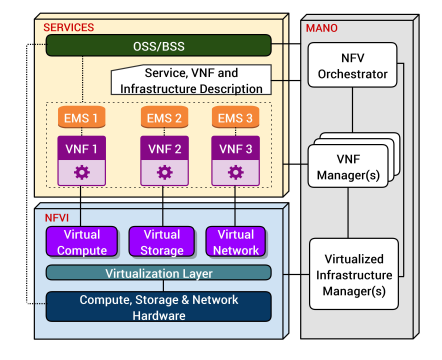
\includegraphics[width=0.8\textwidth]{./fig/NFV}
  \caption{ساختار NFV \cite{NFVArch}}
  \label{fig:NFV}
\end{figure} 
این مؤلفه‌ها به شرح زیر بیان می‌گردد\cite{NFVArch}.
\begin{enumerate}
\item 
خدمات: یک سرویس مجموعه ای از VNF ها است که میتوانند در یک یا چند ماشین مجازی پیاده سازی شوند.
در بعضی مواقع، VNF ها میتوانند در ماشینهای مجازی نصب شده در سیستم عامل یا سخت افزار بطور مستقیم نصب شوند. آنها توسط سرپرستان بومی یا مانیتورهای ماشین مجازی اداره می‌شوند.
معمولاً توسط یک سیستم مدیریت عناصر \LTRfootnote{Element Management System} (EMS)،
 که مسئولیت ایجاد، تنظیمات، نظارت، عملکرد و امنیت آن است، اداره می‌شود.
 EMS 
 اطلاعات ضروری مورد نیاز سیستم پشتیبانی عملیات \LTRfootnote{Operations Support System}(OSS) را در یک محیط SP فراهم می‌کند.
 OSS
  سیستم مدیریت عمومی است، که  همراه با سیستم پشتیبانی از تجارت 
\LTRfootnote{Business Support System}  
  (BSS)
 ، به ارائه دهندگان کمک می‌کند تا چندین سرویس ارتباطی از راه دور را به کار ببندند و مدیریت کنند.
  (به عنوان مثال سفارش، صورتحساب، تمدید، عیب یابی مشکل و غیره).
مشخصات NFV بر ادغام با راه حلهای موجود OSS / BSS متمرکز است.
\item NFVI
:
زیرساختهای NFV تمام منابع سخت افزاری و نرم‌افزاری را که شامل محیط NFV است، پوشش می‌دهد.
NFVI شامل اتصال شبکه بین مکانها، به عنوان مثال، بین
مراکز داده و ابرهای ترکیبی عمومی یا خصوصی است.
منابع فیزیکی به طور معمول شامل محاسبات، ذخیره سازی و سخت افزار شبکه است که وظیفه ی آن پردازش، ذخیره سازی و اتصال VNFها از طریق لایه مجازی سازی است و دقیقاً بالای سخت افزار قرار دارد و منابع فیزیکی را چکیده می‌کند (که به صورت منطقی تقسیم شده و به VNFها اختصاص می‌یابد).
هیچ راه حل خاصی برای استقرار NFV وجود ندارد. در عوض معماری NFV میتواند از یک لایه مجازی سازی موجود مانند Hypervisor با ویژگیهای استاندارد که منابع سخت افزاری را به راحتی استخراج می‌کند و آنها را به VNFها اختصاص می‌دهد، استفاده کند.
وقتی این پشتیبانی در دسترس نباشد، اغلب، لایه مجازی سازی از طریق یک سیستم عامل حاصل می‌شود که نرم‌افزاری را در بالای سرور غیر مجازی یا با اجرای یک VNF به عنوان یک برنامه اضافه می‌کند.
\item NFV-MANO
:
NFV-MANO
 از این موارد تشکیل شده است:
 orchestrator
،
 مدیران VNFs و مدیران زیرساخت مجازی.
 چنین بلوکی عملکردهای مورد نیاز برای کارهای مدیریتی را که برای VNFها اعمال می‌شود، به عنوان مثال تهیه و پیکربندی را  ارائه می‌دهد. 
 NFV-MANO شامل orchestration و مدیریت چرخه منابع فیزیکی یا مجازی است که از مجازی سازی زیرساختها و مدیریت چرخه VNFها پشتیبانی می‌کند.
 همچنین شامل بانکهای اطلاعاتی است که برای ذخیره اطلاعات و مدلهای داده استفاده می‌شود که ویژگیهای چرخه عمر توابع، خدمات و منابع را تعریف می‌کند.
 NFV-MANO روی کلیه وظایف مدیریتی مجازی سازی ویژه لازم در چارچوب NFV تمرکز دارد.
 علاوه بر این، این چارچوب رابطهایی را تعیین می‌کند که میتوانند برای ارتباطات بین مؤلفه‌‌های مختلف
  NFV MANO، 
 و همچنین هماهنگی با سیستمهای سنتی مدیریت شبکه (یعنی OSS و BSS) مورد استفاده قرار گیرند تا امکان عملکرد هر دو VNF و کارکردهای اجرا شده بر روی تجهیزات فراهم شود.
 به طور خلاصه، اگر برش شبکه با استفاده از فایروال و DPI مستقر شده باشد، آنگاه NFV-MANO وظیفه دارد بگوید این VNFها در کجای شبکه فیزیکی قرار دارند. همچنین این VNFها توسط EMS و همان MANO کنترل می‌شوند.
\end{enumerate}
\section{زیرساخت تعریف شده توسط نرم افزار}
زیر‌ساخت تعریف شده توسط نرم‌افزار (SDI\LTRfootnote{Software Defined Infrastructure})
تعریفی از زیرساختهای محاسبات فنی است که کاملاً تحت کنترل نرم افزار بدون دخالت اپراتور یا انسان است.
این عمل مستقل از هرگونه وابستگی خاص سخت افزاری عمل می کند و از لحاظ برنامه قابل توسعه است.
در رویکرد SDI، الزامات زیرساختی یک برنامه به صورت  الزامات کاربردی و غیر عملکردی تعریف شده است به گونه‌ای که می توان به طور خودکار سخت افزار کافی و مناسب برای تحقق این نیازها تهیه کرد.
این زیرساخت شامل شبکه‌ی تعریف شده‌ی نرم‌افزار و شبکه‌ی رادیویی دسترسی تعریف شده‌ی نرم‌افزار می‌باشد که در ادامه توضیح می‌دهیم.
\subsection{شبکه تعریف شده نرم‌افزار (SDN)}
بنیاد شبکه باز 
\LTRfootnote{Open Networking Foundation}
(ONF) 
یک مجموعه ای است که به توسعه، استاندارد سازی و تجاری سازی SDN 
\LTRfootnote{Software Defined Network} 
پرداخت.
ONF
 به طور صریح و دقیق SDN را بدین صورت تعریف کرد:
 شبکه تعریف شده توسط نرم‌افزار (SDN) یک معماری شبکه است که کنترل شبکه از ارسال جدا می‌شود و به طور مستقیم قابل برنامه ریزی است.
 SDN توسط دو ویژگی تعریف می‌شود، یعنی جدا شدن صفحه ی کنترل و داده و قابلیت برنامه ریزی در صفحه کنترل.
 با این وجود، هیچ یک از این دو امضای SDN در معماری شبکه کاملاً جدید نیستند
 \cite{SDN1}.
 SDN 
 در اصل یک الگوی شبکه سازی متمرکز است که در آن هوش شبکه (یعنی عملکرد کنترل یا صفحه کنترل) به طور منطقی در یک یا مجموعه ای از موجودیتهای کنترل (یعنی کنترل کننده‌های SDN) متمرکز می‌شود در حالی که صفحه ی انتقال داده،  ساده و چکیده شده برای برنامه‌‌های کاربردی می‌باشد و سرویسهای شبکه درخواست خود را از طریق کنترل کننده‌های SDN
 بیان میکنند.
 در حالی که در مورد هسته اصلی شبکه موبایل LTE، EPC صحبت میکنیم، مفهوم SDN برای دستیابی به جدایی واضح بین صفحات کنترل و کاربر در اشخاص SGW و PGW استفاده می‌شود.
 با تقسیم دروازه به این روش (یعنی از SGW به SGW-C و
SGW-U 
و از PGW به PGW-C و (PGW-U 
  مقیاس بندی این مؤلفه‌‌ها به طور مستقل امکان پذیر است و طیف وسیعی از گزینه‌‌های استقرار را نیز ممکن می‌کند.
  
 پروتکل مورد استفاده بین صفحه ی کنترل و صفحه ی کاربر میتواند یا افزونه پروتکل موجود OpenFlow باشد، که توسط گروه کاری بی سیم و موبایل ONF (WMWG)با رابطهای جدید، یعنی Sxa و Sxb ساخته می‌شود، که توسط  \lr{3GPP CUPS} تعریف و مشخص می‌شوند\cite{SDN2}. 
 جداسازی صفحه ی کنترل از کاربر منجر به کنترل بیشتر شبکه بوسیله ی برنامه می‌گردد که منجر به بهبود تنظیمات و کارآمدی سیستم می‌گردد.
 SDN
  با ساختار برنامه ریزی شده ی قوانین ترافیک، جایگزین امیدوار کننده ای برای فرماندهی ترافیک ارائه می‌دهد.
  ساختار SDN در شکل \eqref{fig:SDN} آورده شده است.
  \begin{figure}
  \centering
    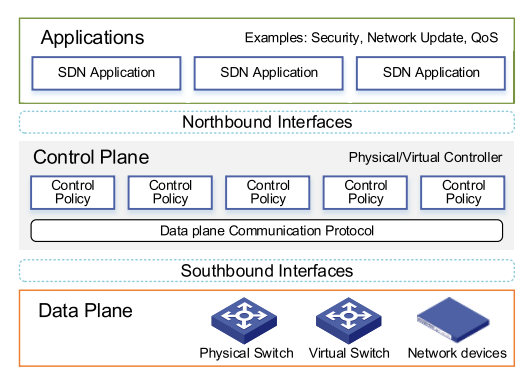
\includegraphics[width=0.8\textwidth]{./fig/SDN}
  \caption{ ساختار SDN \cite{SDN3}}
  \label{fig:SDN}
\end{figure} 
  در این ساختار ۳ لایه ی مختلف وجود دارد که در ادمه بیان میکنیم\cite{SDN3}.
  \begin{enumerate}
  \item لایه ی برنامه :
  این لایه مجموعه ای از برنامه ‌های متمرکز بر خدمات شبکه را پوشش می‌دهد و آنها عمدتا برنامه‌‌های نرم‌افزاری هستند که با لایه کنترل ارتباط برقرار میکنند.
  \item لایه ی کنترل:
  به عنوان هسته اصلی SDN، لایه کنترل از یک کنترلر متمرکز تشکیل شده است که منطقاً نمای شبکه جهانی و پویا را حفظ می‌کند،  که از لایه برنامه درخواست می‌کند و دستگاه‌های شبکه را از طریق پروتکلهای استاندارد مدیریت می‌کند.
  \item لایه ی داده:
  این لایه، زیرساختها شامل سوئیچها، روترها و لوازم شبکه می‌باشد. در زمینه SDN، این دستگاه‌ها قابل برنامه ریزی هستند و از رابطهای استاندارد پشتیبانی میکنند.
  \end{enumerate}
\subsection{شبکه دسترسی رادیویی تعریف شده نرم‌افزار (SDRAN)}
SDRAN \LTRfootnote{Software Defined Radio Access Network}
یا شبکه‌ی دسترسی رادیویی تعریف‌ شده‌ی نرم‌افزار، یک بازنگری اساسی در لایه دسترسی رادیویی است.
SDRAN
یک صفحه‌ی کنترل متمرکز نرم‌افزار تعریف شده است برای بخش شبکه دسترسی رادیویی که ایستگاه‌های پایه را در یک مکان جغرافیایی داخلی، به عنوان یک ایستگاه پایه‌ی بزرگ مجازی با المانهای کنترلی مرکزی و رادیویی می‌باشد.
در این حالت، مفهوم SDRAN به مفهوم vRAN بسیار نزدیک است.
SDRAN
 صفحه کنترل و صفحه داده را در
 RAN 
 جدا می‌کند و تصمیمات کنترل را به صفحه کنترل متمرکز می‌کند. در معماری های رایج SDRAN، یک کنترل کننده مرکزی اطلاعات کل شبکه را جمع می کند و در سطح کلی برای هر عنصر صفحه داده تصمیم گیری می‌کند. این روش از سربار شدن تصمیم گیری در عناصر صفحه داده جلوگیری می‌کند و فرصتی را برای مدیریت انعطاف پذیر و هماهنگ در کل RAN فراهم می‌کند.
در تعریف چنین معماری، ما چارچوبی ایجاد می‌کنیم که از طریق آن یک شبکه جغرافیایی محلی می‌تواند به طور موثر توازن بار و مدیریت تداخل را انجام دهد و همچنین نرخ عملیاتی و یا هر هدف دیگر را به بهینه‌ترین مقدار خود برساند.
ما معتقدیم که طراحی تعریف شده توسط نرم افزار در RAN یک گام اساسی برای پشتیبانی از برش شبکه، به اشتراک گذاری RAN، مدیریت طیف انعطاف پذیر و سایر ویژگی های اصلی در شبکه های 5G خواهد بود.
امید بر این است که طراحی تعریف شده توسط نرم افزار در RAN 
(SDRAN) 
یک گام اساسی برای پشتیبانی از برش شبکه، به اشتراک گذاری RAN، مدیریت طیف انعطاف پذیر و سایر ویژگی های اصلی در شبکه های 5G خواهد بود
\cite{gudipati2013softran,yu2017hsdran}. 

 \section{برش شبکه}
 پیش بینی می‌شود شبکه‌‌های \lr{5G} چندین سرویس را با نیازهای مختلف به طور همزمان پشتیبانی کند.
 برش شبکه
 \LTRfootnote{Network Slicing}
به عنوان راه حلی برای چنین تقاضا در نظر گرفته شده است.
یک برش شبکه، یک شبکه منطقی \lr{end-to-end} است که خدمات  با نیازهای خاص را ارائه می‌دهد.
 چندین برش شبکه
در یک زیرساخت یکسان
  اجرا و مدیریت می‌شوند و
به طور مستقل کار میکنند.
برش شبکه
 با هدف تقسیم منطقی مجموعه توابع و منابع شبکه در یک نهاد شبکه در نظر گرفته شده است که مطابق با خواسته‌‌های فنی یا تجاری خاص می‌باشد.
 با خرد کردن یک شبکه فیزیکی به چندین شبکه منطقی، برش شبکه میتواند از خدمات متناسب با تقاضا برای سناریوهای برنامه مشخص در همان زمان با استفاده از همان شبکه فیزیکی پشتیبانی کند.
با استفاده از برش شبکه، منابع شبکه میتوانند به صورت پویا و کارآمد به برشهای شبکه منطقی با توجه به خواسته‌‌های QoS مربوطه اختصاص داده شوند\cite{NS1}. 

\begin{figure}
  \centering
    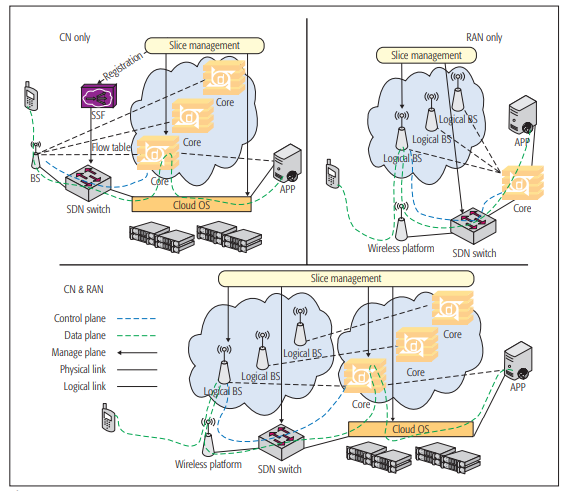
\includegraphics[width=0.8\textwidth]{./fig/NS}
  \caption{سه ساختار برش شبکه \cite{NS2}}
  \label{fig:NS}
\end{figure} 
پیاده سازیهای مختلفی از برش شبکه وجود دارد که شامل برش هسته ی شبکه، برش \lr{RAN} و برش هر دو بخش می‌باشد\cite{NS2}.
\begin{itemize}
\item \textbf{برش هسته:}
هسته ی شبکه (CN) \LTRfootnote{core network}
به عنوان برشهای شبکه، مجازی سازی می‌شوند که با ویژگیهایی مانند ویژگیهای قابل برنامه ریزی و قابل اعتماد بودن که شامل مدیریت حرکت و تأیید اعتبار می‌باشد.
برشهای شبکه فقط در CN وجود دارد.
  بنابراین، نه RAN و نه تجهیزات کاربر (UE) برای CNهای برش داده شده نیاز به تنظیم ویژه ندارند.
  در برش هسته ی شبکه، برش تنها در بخش هسته ی شبکه است و تمام واسطها و فرآیندها، بدون تغییر باقی میمانند
  به جز مواردی که در ابتدا UEها به شبکه‌‌ها وصل می‌شوند، زیرا UEها باید به برش صحیح CNها اختصاص داده شوند.
\item \textbf{
برش شبکه ی دسترسی رادیویی:
}
برخلاف برش CN،
برشهای RAN روی سخت افزار رادیویی و استخر منابع باند پایه، به نام یک سطح بی سیم، اجرا می‌شوند که دارای کشش کمتری نسبت به زیرساخت مجازی بالغ شده در CNها هستند.
با چند BS منطقی، برشهای RAN پارامترهای مختلفی از رابطهای هوا (به عنوان مثال، طول نماد، فاصله زیر حامل، طول پیشوند چرخه و پارامترهای درخواست تکرار خودکار هیبریدی \LTRfootnote{HARQ}) را اعمال می‌کند.
علاوه بر این، پارامترهای دیگری مانند انتخاب سلول و آستانه انتقال، و همچنین سیاستهای انتقال هماهنگ را میتوان برای هر برش تعریف کرد تا یک تجربه بی سیم برجسته را به کاربران ارائه دهد.
\item \textbf{برش هسته و شبکه ی دسترسی رادیویی}:
در این سناریو، هر برش از RAN به یک برش از هسته متصل می‌شود، بنابراین اپراتورها میتوانند یک شبکه منطقی انتهای به مشتریان ارائه دهند.
روش انتخاب برش همان روش برش RAN است، بنابراین کاربران پس از دسترسی به سیستم، نیازی به انتخاب برش CN ندارند.
این مدل از برش مزایای هر دو مدل از برش را باهم دارد.
 در نتیجه این روش برش، قادر به برنامه ریزی ویژگیهای CN و همچنین دارای قابلیت تغییر رابطهای هوایی RAN
 می‌باشد.
 
\end{itemize}


\section{دستاوردهای پروژه}
در اینجا، هدف در نظرگیری ساختار رادیویی دسترسی باز در نسل پنجم و تخصیص منابع آن می‌باشد.
مسئله‌ی برش شبکه در بخش رادیویی و قرارگیری توابع مجازی شبکه برروی مراکز داده باهم در شبکه‌ی دسترسی رادیویی باز مورد بررسی قرار گرفته است. بخش رادیویی به صورت کامل مدل سازی شده و تاخیر و نرخ و پارامترهای دیگر بدست می آید. در اینچا فرض براین است که کاربران بر اساس سرویس مورد نیاز، دسته بندی می شوند و هدف تخصیص منابع فیزیکی محاسباتی به این برشهای اختصاص یافته به سرویسها می باشد.
برای حل این مسئله، ابتدا مسئله را به دو مسئله‌ی کوچکتر مختلف شکسته که در مرحله اول، برای یافتن تخصیص توان، تخصیص PRB و تعداد VNF ها، مسئله را دوباره فرموله و ساده می کنیم. در مرحله دوم، ارتباط O-RU حل می شود.
در این مسئله، تاخیر و نرخ هر کاربر در سرویس مورد بررسی قرار گرفته شده و چالش تخصیص منابع که شامل برش بخش رادیویی به هر سرویس است و جاگیری توابع شبکه حل می‌شود. 
\section{ساختار پروژه}
در این فصل مروری بر مفاهیم مورد استفاده در پروژه کردیم.
در فصل دوم مروری بر ادبیات پیشین و خلاصه‌ای از مدل سیستم مقالات موجود، بیان می‌گردد. در این فصل ابتدا صورت مسئله‌ی برش شبکه، شبکه‌های دسترسی رادیویی باز و قرارگیری توابع شبکه در مراکز دادهِ و آسیب پذیری‌های این سیستم و مسايل مربوط به امنیت سیستم را بررسی کرده سپس در مورد حل مسئله صحبت می‌کنیم.
در فصل سوم مدل سیستم در نظر گرفته بیان می‌شود و صورت مسئله به نمایش گذاشته می‌شود و روشهای حل آن بیان می‌گردد. همچنین  نتایج شبیه سازی قرار داده می‌شود.
در فصل چهارم صورت مسئله را ساده‌سازی کرده و با روش دینامیکی مسئله را با در نظر گرفتن امنیت سیستم حل می‌نماییم.
در فصل پنجم نیز نتیجه گیری و کارهای آتی مورد نظر و پیشنهادات بیان می‌شود.   
\section{نتیجه گیری}
در این فصل ابتدا مروری بر تاریخچه ی مخابرات و نسلهای چهارم تا ششم مخابراتی شد. سپس ساختارهای مختف دسترسی رادیویی به طور خلاصه بیان شد و در نتیجه ی آن ساختار CRAN که ساختار ابری است تعریف شد. سپس ساختار xRAN
مورد توجه قرار گرفت و در نهایت ساختار ORAN 
که ترکیب و تکاملی از CRAN و xRAN می‌باشد مورد توجه قرار گرفت.
سپس به مرور آسیب پذیری‌های ORAN و مسئله‌ی امنیت آن پرداخته شد.
بعد از بیان ساختارهای رادیویی، ساختار هسته ی شبکه را در نسل پنجم بیان کردیم که شامل 
NFV و SDN 
می‌باشد که منجر به جداسازی صفحه ی کنترل از کاربر می‌شود و سیستم هوشمندتر همراه با قابلیت برنامه ریزی بیشتر می‌گردد.
در ادامه برش شبکه در بخش رادیویی و هسته و هردو مورد توجه قرار گرفته شد.
%سپس در مورد دو مسئله‌ی NP-Hard صحبت نمودیم. در نهایت در مورد دستاوردهای پروژه و ساختار فصلهای آتی صحبت می‌نماییم. 		% فصل اول: مقدمه
\chapter{مروری بر کارهای پیشین}

\section{مقدمه}
در این فصل، به مرور کارهای گذشته می‌پردازیم.
ابتدا صورت مسئله مقالات مختلف را بررسی می‌نماییم که
 به ترتیب شامل مقالاتی هستند که از برش شبکه استفاده کرده اند.
برش شبکه در سه بخش رادیویی، بخش هسته و هردو بخش هسته و رادیویی صورت می‌گیرد.
سپس در زمینه ی سیر عبور از شبکه های دسترسی رادیویی ابری به شبکه های دسترسی رادیویی باز مطالعه نموده و بعد از آن درباره ی جاگیری VNF ها صحبت می‌کنیم.
سپس در مورد روش حل مسئله صحبت می‌کنیم که شامل مسائل کوله پشتی و بسته بندی جعبه می‌باشد و در نهایت در مورد روشهای یادگیری تقویتی صحبت می‌کنیم.
\section{مروری بر مسائل پیشین}
در این بخش به مطالعه ی مقالات متشابه می‌پردازیم. ‌‌‌ابتدا در مورد مسائل مرتبط با برش شبکه صحبت نموده سپس در مورد شبکه‌های دسترسی رادیویی باز مطالعه نموده و در نهایت به مروری بر کارهای انجام شده در زمینه‌ی قرارگیری توابع شبکه‌ی مجازی می‌پردازیم.
\subsection{برش شبکه}
برش شبکه یک شبکه منطقی انتها به انتهای مستقل است که بر روی یک زیرساخت فیزیکی مشترک کار ‌ و قادر به ارائه خدمات می‌باشد.
در این بخش برش شبکه در بخش رادیویی و هسته و هردو را بررسی می‌کنیم.
%\subsection{برش شبکه در شبکه های دسترسی رادیویی }

مشکل تخصیص منابع برای برش شبکه در شبکه های سلولی چند مستاجر اخیرا مورد توجه قرار گرفته است\cite{feng2020dynamic,lee2018dynamic,lee2016new}.

برش RAN یکی از کلیدهای اصلی برای انعطاف پذیری سفارشات و مدیریت مجازی سازی ایستگاه پایه می‌باشد تا بتواند منابع رادیویی را در میان سرویس های مختلف تقسیم کرده و منجر به سازگاری اپراتورها و برطرف کردن نیاز سرویس ها گردد.
%در ادامه مروری بر این مدل مقالات می‌نماییم.
%\subsubsection{  برش شبکه در شبکه های دسترسی رادیویی ابری و متجانس و مهی}

شبکه های دسترسی رادیویی ابر (C-RAN) به عنوان یک چارچوب امیدوار کننده برای سیستم های ارتباط بی سیم نسل پنجم ظاهر شده‌اند.
از آنجا که آنها میتوانند پیچیدگی رمزگشایی، مصرف انرژی و دخالت های ناشی از افزایش تراکم تلفن همراه را کاهش دهند\cite{cranInt}.
در ادامه در مورد برش شبکه در بخش رادیویی شبکه های دسترسی رادیویی ابری صحبت می‌کنیم.

در مقاله‌ی \cite{lee2018dynamic}
برش شبکه به صورت دینامیکی در بخش رادیویی مورد بررسی قرار گرفته شده‌است.
برش شبکه در اینجا به عنوان فرآیند تخصیص منابع شبکه به کاربران انجام ‌
چارچوب طرح برش شبکه شامل یک سطح بالاتر، که مدیریت کنترل پذیرش کاربران، ارتباط کاربر که شامل تخصیص واحد رادیویی (RRH) برای بیشینه سازی نرخ کاربران و تخصیص ظرفیت منابع باند پایه (‌BBU) و یک سطح پایین تر، که تخصیص توان و بلوک منابع فیزیکی (PRB) در میان کاربران می‌باشد.
در این مدل فرض می‌کنیم که هر سرویس دارای شبکه اصلی خود (یا قطعه اصلی شبکه) است که به H-CRAN متصل می‌شود.
سلول بزرگ RRH (M-RRH) و سلولهای کوچک RRHs (S-RRHs) به ترتیب از طریق پیوندهای پشتی و fronthaul به یک استخر ابر
BBU  متصل میشوند.
همچنین ، تقسیم C/U در مدل سیستم فرض می‌شود، که به موجب آن صفحات کنترل و داده از هم جدا میشوند به گونه ای که صفحات کنترل توسط M-RRH در شبکه مدیریت می‌شود.
\begin{figure}%[H]
  \centering
    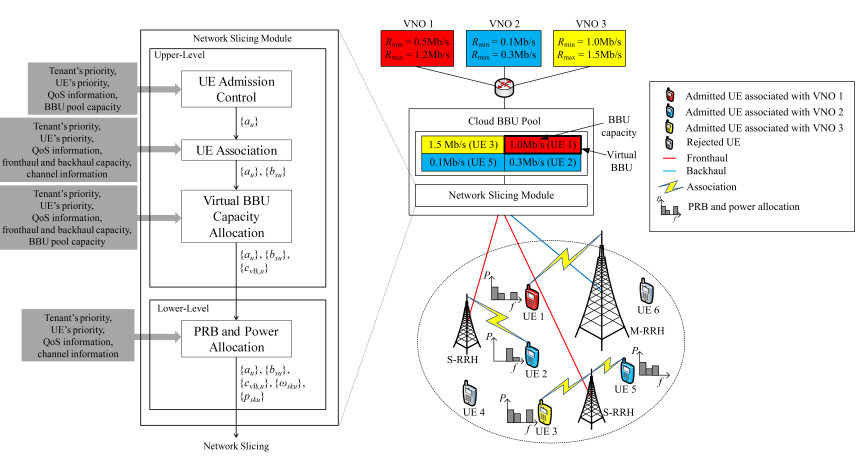
\includegraphics[scale = 0.7]{./fig/dynamicNS}
  \caption{روند برش شبکه\ \cite{lee2018dynamic}}
  \label{fig:dns}
\end{figure}
%برای حل این مسئله، میبایست مسئله را به بخش های کوچکتر تقسیم کرده و حل نماییم.
همانطور که در شکل \eqref{fig:dns} 
مشخص شده‌است ابتدا پذیرش کاربر مورد توجه قرار می‌گیرد و سپس کاربر به RRH متصل می‌شود و پس از آن ظرفیت BBU به آن تخصیص می‌دهد که تا این بخش از کار در سطح بالا قرار داریم.
در سطح بالا، یک مسئله کنترل پذیرش با برنامه نویسی پویا می‌باشد که در آن پیچیدگی را میتوان تنظیم کرد.
این مسئله از جنس مسئله ی
کوله پشتی \LTRfootnote{Knapsack}
باینری
 می‌باشد که با الگوریتم دینامیکی جواب بهینه ی آن بدست میآید.
همچنین مسئله ی ارتباط کاربر نیز یک مسئله ی کوله پشتی باینری است که با استفاده از یک الگوریتم حریص با پیچیدگی کم بهینه و حل می‌شود.
 مسئله ی تخصیص ظرفیت BBU نیز فرموله شده و با برنامه ریزی خطی حل می‌شود.
 حال وارد الگوریتم سطح پایین تر میشویم که تخصیص توان و منبع فیزیکی می‌باشد.
برای مساله ی سطح پایین تر، مشکل تخصیص منابع به عنوان یک مشکل برنامه نویسی mixed-integer غیر محدب است که با استفاده از روش دوگانه لاگرانژ حل می‌شود.

در مقاله‌ی 
\cite{larsen2018fronthaul,costanzo2018network}
برش شبکه در شبکه های دسترسی رادیویی ابری مورد توجه قرار گرفته است. 
در بخش fronthaul مشکلاتی از قبیل پیچیدگی شبکه و محدودیت نرخ وجود دارد که در برش شبکه، منجر به بهبود آن می‌شود.
علاوه بر این ، C-RAN میتواند مجازی سازی مجموعه ای از توابع RAN را امکان پذیر کرده و راه را برای اصطلاحاً RAN مجازی باز کند. با این کار میتوان چندین شبکه مجازی یا برش ایجاد کرد.
 مقاله‌ی
\cite{larsen2018fronthaul}
نشان داده است که استفاده از برش شبکه و برخورداری از سوییچ بسته در fronthaul
مزایای زیادی را به همراه خواهد داشت که از جمله برخورداری از تقسیمات عملکردی مختلف خواهد بود. همچنین از معایب این کار تاخیر نسبتا اندکی می‌باشد.

در مقاله‌ی 
\cite{fran}
برش شبکه در بخش رادیویی برای ساختار مه \LTRfootnote{Fog Radio Access Network}
 یا F-RAN
  در نظر گرفته شده‌است که در آن دو نمونه برش شبکه برای هات اسپات و سناریوهای وسیله نقلیه با زیرساخت مربوط تنظیم می‌شود. به طور خاص ، چارچوب برای برش RAN به عنوان یک مشکل بهینه سازی مشترک برای مقابله با ذخیره کردن و انتخاب حالت است.
  با توجه به خواسته های کاربران مختلف و منابع محدود، پیچیدگی مسئله بهینه سازی اصلی بسیار زیاد است و همین امر باعث می‌شود که رویکردهای بهینه سازی سنتی به طور مستقیم سخت باشد.
 برای مقابله با این معضل ، یک الگوریتم یادگیری تقویت عمیق ارائه شده‌است ، که ایده اصلی آن این است که سرور ابر تصمیمات صحیحی را در زمینه ذخیره محتوا و انتخاب حالت برای به حداکثر رساندن عملکرد پاداش در وضعیت کانال پویا و وضعیت حافظه نهان ارائه می‌دهد.
%\subsubsection{برش شبکه در شبکه های دسترسی رادیویی }

در مقاله‌ی 
\cite{ranSlice, ranSlice1}
اجرای مفهوم برش در سطح RAN توسط اپراتور شبکه تلفن همراه (MNO) برای پاسخگویی به نیازها می‌باشد. همچنین مساله ی تخصیص منابع (در اینجا پهنای باند) مورد توجه قرار گرفته شد.
چالش های پیش رو برش RAN نیز مورد بررسی قرار گرفته است که یکی از چالش ها
شامل طراحی و مدیریت چندین برش در زیرساخت مشترک به روشی کارآمد و در عین حال ضمانت SLA توافق شده برای هر یک از آنها است.
این چالش ما را نیازمند مفهوم ایزولاسیون برش می‌کند.

در مقاله‌ی 
\cite{ranslice2}
برش در بخش RAN مورد توجه قرار گرفته است.
همچنین
در این مقاله‌یک برنامه تخصیص منابع پویا، با هدف به طور مشترک بهینه سازی مصرف برق و تخصیص پهنای باند در حالی که رضایت از تأخیر مربوطه برای ورود ترافیک پراکنده uRLLC و کیفیت خدمات eMBB را تا حد ممکن ارائه می‌دهد، پیشنهاد می‌کند.
طرح پیشنهادی براساس کنترل بهینه توان برای تخصیص منابع آگاه از تأخیر است.
در نتیجه در این سیستم هدف مینیمم کردن توان با شروط برآورده شدن شروط پهنای باند و  تاخیر که با شرط صف پردازش نشان داده، می‌باشد.
%\subsection{برش شبکه در بخش هسته  }

در مقاله‌ی 
\cite{onet}
اجرای عملی برش شبکه پیشنهاد شده‌است.
در مدل پیشنهادی، نویسندگان فرض میکنند که در هر شکاف زمانی مشخص، کاربران فقط میتوانند یک برش شبکه واحد را درخواست کنند.
در اینجا تابع هدفی بر اساس نسبت میزان منابع اختصاص داده شده به کاربرن در هر زمان t به ظرفیت کل منابع مشخص شده‌است و هدف بیشینه سازی آن  می‌باشد.  
مدل پیشنهادی بر اساس مسئله \lr{multi armed bandit} ساخته شده‌است و نویسندگان سه نوع  آن را برای حل جنبه های مختلف تخصیص برش شبکه معرفی کرده اند.
آنها با استفاده از MATLAB مدل بهینه سازی را شبیه سازی کرده و نتایج را با یک الگوریتم حریص مقایسه کردند. آنها همچنین اثبات مفهوم برش شبکه را ارائه دادند.

برش شبکه یکی از فناوری های کلیدی است که به شبکه های 5G اجازه می‌دهد منابع اختصاصی به صنایع مختلف (خدمات) ارائه دهند.
در مقاله‌ی
\cite{li2019latency}
نویسندگان یک روش تخصیص منابع (تأخیر بهینه) برای برشهای شبکه حمل و نقل 5G برای پشتیبانی از خدمات URLLC ارائه داده اند.
آنها ویژگی های منبع شبکه و ویژگی های توپولوژی تخصیص منابع در تقسیم شبکه را معرفی کردند.

در 
\citep{vnf1,coreSlice}
ایزوله کردن برش شبکه ی هسته 
مورد توجه قرار گرفته است.
\citep{vnf1}
برای کاهش تأثیر حملات DDoS در احراز هویت برش ، از ایزوله کردن برش شبکه ی هسته استفاده شده و حل آن با ترکیبی از شبیه سازی و یک آزمایش عملی ارزیابی شده‌است.
نویسندگان
\citep{coreSlice}
دو چالش مهم برش شبکه در بخش هسته مورد توجه قرار داده اند که شامل ایزوله کردن برش شبکه و تضمین میزان تاخیر انتها به انتها می‌باشد.
در این مقاله، مساله ی بهینه سازی به صورت 
\lr{mixed integer linear programming}
 می‌باشد که
 تابع هدف درخواست های برش ورودی را به سروری که کمترین میزان استفاده از آن شده‌است، اختصاص داده و مسیری را با حداقل تأخیر پیدا می‌کند. خروجی این مساله VNF ها را به سرور اختصاص می‌دهد.  
%\subsection{برش شبکه در هسته و بخش رادیویی}

در این دسته مقالات، سرویس ها به دو بخش تقسیم میشوند در بخش اول سرویس هایی که  نسبت به تاخیر حساسند و دسته ی دوم سرویس هایی که نسبت به نرخ انتقال حساسند. همچنین در برخی مقالات هر دو ویژگی برای یک سرویس مد نظر می‌باشد.
در این مدل های سیستم، تاخیر با استفاده از M/M/1 در ساده ترین حالت یا برای نزدیک تر شدن به حالت حقیقی از M/D/1 نیز استفاده می‌شود. میتوان در این مدل ها تاخیر را کمینه و نرخ انتقال را بیشینه کرده و یا 
برای کاربران نرخ را از حد مورد نیاز بیشتر و تاخیر را کمتر از حد مورد نیاز فرض کرد\cite{frdl,luong2018novel,luong2018novel1,guo2016exploiting}.
 \begin{figure}%[H]
  \centering
    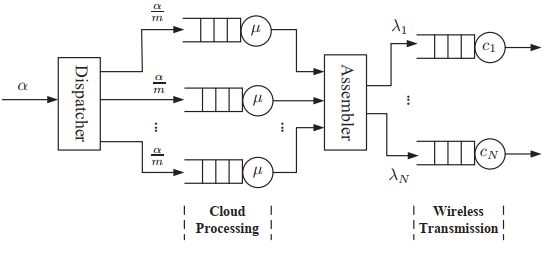
\includegraphics[scale = 0.7]{./fig/Delay}
  \caption{مدل پردازشی شبکه صف \cite{frdl}.}
  \label{fig:Delay}
\end{figure}
همانطور که در شکل \eqref{fig:Delay}، مشخص است، در این شبکه برای هر بخش تعدادی VNF قرار دارند که پردازش ها را انجام می‌دهند. در مسیر لینک پایین
بسته ها با نرخ $\alpha$ به صف های مختلف وارد شده و پس از پردازش با همدیگر ادغام شده و سپس بسته ی هر کاربر از طریق وایرلس منتقل میشوند.
در این پردازش ها، از روش M/M/1 استفاده شده‌است.
در این مدل مقالات اشاره ی مستقیم به برش شبکه نشده‌است ولی
در آنها ترکیبی از مفهوم برش RAN و Core به چشم می‌خورد.
\subsection{همزمانی سرویسهای eMBB و URLLC}
یکی از موضوعات چالش‌برانگیز، چندگانه سازی 
\LTRfootnote{multiplexing}
 سرویس های eMBB و URLLC در یک RAN و به اشتراک گذاری منابع این سرویس ها می‌باشد که بسیاری از محققان به این موضوع توجه دارند.
 در \cite{setayesh2020joint,yang2020should,saggese2021power}، مشکل تخصیص منابع در همزیستی خدمات URLLC و eMBB بر اساس QoS آنها در نظر گرفته شده است.
 در \cite{alsenwi2021intelligent}، مشکل تخصیص منابع برای سرویس‌های مشترک eMBB و URLLC با یادگیری تقویتی عمیق فرمول‌بندی و حل می‌شود.
 در \cite{korrai2020ran}، نویسندگان پیشنهاد کردند که منابع RAN برای سیستم برش شبکه در همزیستی خدمات eMBB و URLLC تخصیص داده شود. این سیستم تاخیر، نرخ سرویس و حفظ قابلیت اطمینان را تضمین می کند.
\subsection{ شبکه های دسترسی رادیویی باز}
در فوریه 2018 ، شبکه دسترسی رادیویی آزاد (ORAN) با ادغام  xRAN و اتحاد C-RAN برای ایجاد سطح جدیدی از باز بودن در شبکه دسترسی رادیویی ایجاد شد که از نسل 5G و 6G پشتیبانی می‌کند.
هدف اصلی ORAN افزایش عملکرد RAN از طریق عناصر شبکه مجازی و واسط های باز است که دارای هوش در RAN است.
صراحت و هوش دو ستون اصلی تلاشهای انجام شده توسط اتحاد ORAN است که یک نیروی جهانی متشکل از بیش از 160 شرکت کننده از فروشندگان بزرگ ، شرکت های کوچک و متوسط ، اپراتورهای شبکه ، مبتدیان و مؤسسات دانشگاهی است
\cite{oranpaper}
.

در مقاله‌ی 
\cite{oranInt}
 مقدمه ای در مورد مفاهیم، اصول و الزامات \lr{Open RAN} که توسط اتحاد ORAN مشخص شده، بیان شده‌است.
 در این مقاله،
 به منظور نشان دادن نقش هوش در ORAN، طرح مدیریت منابع رادیویی هوشمندی را برای رسیدگی به ازدحام ترافیک و نشان دادن اثربخشی آن در یک مجموعه داده در دنیای واقعی پیشنهاد شده‌است.
 یک معماری سطح بالا از این سناریوی استقرار که سازگار با الزامات ORAN است نیز مورد بحث قرار گرفته است. مقاله با چالشهای کلیدی فنی و مشکلات باز برای تحقیقات و توسعه آینده به پایان میرسد.
 
در مقاله‌ی
\cite{c2o}
تعاریف عمومی، ویژگی های اساسی و روند تحقیقاتی فعلی در شبکه های دسترسی رادیویی ابری و مشتقات آن، شبکه های دسترسی رادیویی مجازی و شبکه های دسترسی رادیویی باز ارائه شده‌است.
علاوه بر این، نتایج عملی و آموزه های آموخته شده در مورد محدودیت ها و مسائل پیش بینی نشده مجازی سازی شبکه های دسترسی رادیویی را ارائه داده شده‌است.

در مقاله‌ی 
\cite{sree2019open, kawahara2019ran}
 ساختار و مدیریت منابع رادیویی (RRM) هوشمند 
 و همچنین نقش مدیریت لینک رادیویی (RLM) در بهینه سازی انرژی در RRM
در نظر گرفته شده‌است.
ساختار RLM در 
زیرساخت ORAN مورد بررسی قرار گرفته است.
علاوه بر این، دیدگاه
O-RAN
 و معماری آن مورد توجه قرار گرفته است.
\subsection{قرار دادن VNF ها}
NFV
 الگویي است که عملکردهای شبکه سنتی را مجازی می‌کند و آنها را در سخت افزارهای عمومی و ابرها در مقابل سخت افزارهای تعیین شده، قرار می‌دهد.
 در واقع NFV بخش نرم افزار را از سخت افزار جدا می‌نماید.
 بنابراین یک سرویس داده شده میتواند به مجموعه ای از توابع شبکه مجازی (VNF) تجزیه شود ، سپس میتوان آن را در نرم افزارهایی که روی یک یا چند سرور استاندارد فیزیکی صنعت اجرا میشوند ، پیاده سازی کرد.
 
اپراتورهای شبکه تلفن همراه عهده دار تصمیم گیری مدیریت زیرساخت است.
این وظیفه بخشی از تنظیمات شبکه است و شامل تصمیم گیری در مورد قرار دادن VNF های مورد نیاز در سراسر زیرساخت و اختصاص پردازنده، حافظه و منابع ذخیره سازی به VNF ها و مسیریابی داده ها از طریق گره های شبکه
می‌باشد.

به لطف برش شبکه، شبکه های 5G از انواع خدمات به روشی انعطاف پذیر و سریع پشتیبانی میکنند. در این زمینه ، ما به دنبال تصمیم گیری بهینه و با کیفیت بالا در مورد قرار دادن VNF در میان میزبانهای فیزیکی برای تحقق بخشیدن به خدمات هستیم.

در مقالات
\cite{wang2016online,jia2018online,luo2020online}
هدف یافتن تعداد بهینه ی VNF ها در یک زنجیره ی سرویس و قرار گیری VNF های مورد نظر بر روی سرور در هر بازه ی زمانی می‌باشد تا بتوان میزان هزینه را در سیستم به حداقل رساند.
در این مقالات هدف کمینه کردن انرژی های مصرفی در هر بازه ی زمانی می‌باشد که شامل هزینه ی انرژی مصرفی هر VNF مستقر بر روی سرور در حال کار و هزینه ی استقرار VNF های جدید در هر لحظه ی زمانی می‌باشد.
همچنین مجموع منابع مصرفی VNF های مستقر بر روی هر سرور در هر لحظه میبایست از منابع آن سرور کمتر باشد تا مساله عملی شود.
با استفاده از الگوریتم آنلاین این مساله حل شده‌است.‌
در مقاله‌ی 
\cite{jia2018online,luo2020online}
نرخ جریان هر VNF و سرور نیز در نظر گرفته شده‌است و دیتا سنترها و VNF ها به صورت گرافی شبیه سازی شده‌اند.
در مقاله‌ی
\cite{luo2020online}
الگوریتم روند کردن استفاده کرده که نتیجه ی خوبی را در مقابل مساله ی آفلاین دارد.

در مقاله‌ی
\cite{cziva2018dynamic}
مساله ی قرار دادن VNF ها در لبه مورد بررسی قرار می‌گیرد که در اینجا تخصیص VNF ها در یک سیستم با زیرساخت لبه مورد توجه قرار گرفته است و هدف کمینه کردن تاخیر انتها به انتها از هر کاربر به VNF مورد نظر آن می‌باشد و از روش دینامیکی و پویا برای حل مساله استفاده شده‌است. 

در مقاله‌ی
\cite{pei2019optimal}
مساله ی قرار دادن VNF در شبکه های فعال SDN/NFV مطالعه شده‌است، که به طور طبیعی به عنوان یک مساله ی برنامه نویسی باینری (BIP) فرموله شده‌است. 
در این مساله قرارگیری VNF زنجیر عملکرد سرویس مورد بررسی قرار گرفته شده‌است. 
با استفاده از روش یادگیری تقویت عمیق، الگوریتم قرارگیری VNF مبتنی بر شبکه DDQN \LTRfootnote{Double Deep Q-learning} پیشنهاد می‌کنیم.

در مقاله‌ی
\cite{ren2020joint}
 مسئله ی بهینه سازی مشترک قرار دادن VNF ها و زمانبندی جریان مطالعه شده‌است.
 این مساله از نوع برنامه نویسی عدد صحیح می‌باشد.
 برای حالت تک جریان، مساله به سادگی قابل حل است اما برای جندین جریان مساله
 NP-hard
 خواهد بود و با استفاده از روش relax کردن لاگرانژ
 قابل حل می‌باشد.
\section{روش های حل}
در این بخش مروری بر حل مسائل توسط مقالات می‌نماییم. 
ابتدا به دو مسئله ی معروف NP-Hard
اشاره می‌کنیم سپس به حل مسائل با استفاده از روش یادگیری تقویتی می‌پردازیم.
\subsection{مسئله‌ی کوله‌پشتی و بسته‌بندی جعبه}
در اینجا به دو مسئله‌ی کوله پشتی و بسته بندی جعبه می‌پردازیم. این دو مسئله NP-Hard هستند.
مسئله‌ی NP-hard را نمی‌توان در زمان چند جمله‌ای حل کرد در نتیجه از روشهای ابتکاری برای رسیدن به جواب نزدیکه بهینه استفاده می‌شود.
\subsubsection{ مسئله‌ی کوله‌پشتی }
یکی از مسائل پیش رو، مسئله ی کوله پشتی \LTRfootnote{knapsack}
می‌باشد.
این مسئله، از جنس NP-hard
می‌باشد که در این مسئله میخواهیم تعدادی شی با وزنهای مختلف را در تعدادی جایگاه با ظرفیت مشخص قرار دهیم.
هدف در این مسئله قرارگیری بیشترین تعداد اشیاء در این جایگاه ها می‌باشد.
حل این مسئله با استفاده از روش های مختلف صورت می‌گیرد.

در مقاله‌ی \cite{lee2018dynamic}
همانطور که قبل تر اشاره شد، مسئله ی پذیرش کاربر و ارتباط کاربر از جنس کوله پشتی
 می‌باشد که به ترتیب با استفاده از الگوریتم دینامیکی و الگوریتم حریص تعریف شده در مقاله
 حل می‌گردد.

در مقاله‌ی
\cite{sciancalepore2017mobile}
یک راه حل جامع شامل برش شبکه، پیش بینی ترافیک، کنترل پذیرش و برنامه ریزی برای یک سیستم شامل برش شبکه 5G ارائه شده‌است.
راه حل کنترل پذیرش به یک مسئله کوله پشتی هندسی (دو بعدی) ترسیم شده و دو الگوریتم کم پیچیدگی به ترتیب برای درخواست های برش شبکه منظم و نامنظم طراحی شده‌اند. 
\subsubsection{مسئله‌ی بسته‌بندی جعبه}
 در این مسئله هدف قرار دادن تعدادی شیء در تعدادی جعبه با ظرفیت مشخص می‌باشد.
در مسئله ی بسته بندی جعبه \LTRfootnote{bin packing}
هدف کمینه کردن تعداد جعبه های ورودی با فرض اینکه همه ی اشیا در آن جا شوند.

در مقاله‌ی
\citep{wang2017joint}
مسئله ی تخصیص منابع و بدست آوردن انرژی بهینه در ساختار
H-CRAN
می‌باشد.
در این مقاله هدف تخصیص همزمان منابع ایستگاه رادیویی RRH و باند پایه BBU می‌باشد.
این مسئله به دو بخش مجزا برای تخصیص منابع هر بخش شکسته می‌شود.
بخش دوم که مربوط به زمان بندی و برنامه ریزی BBU می‌باشد به فرم یک مسئله ی باینری بسته بندی جعبه نوشته می‌شود.
برای حل این الگوریتم از روش های مختلفی از جمله
Next-Fit(NF)
First-Fit(FF)،
First-Fit-Decreasing(FFD)،
و
‌Best-Fit-Decreasing(BFD)
می‌باشد که الگوریتم به کار رفته در مسئله از نوع روش
BFD 
 است که جواب بهتری در مقایسه با روشهای دیگر دارد.  
 
در مقاله‌ی
\cite{de2020optimal}
به صورت همزمان قرار دادن VNF ها و تخصیص منابع محاسباتی مورد هدف قرار داده شده‌است.
این مسئله به صورت
برنامه نویسی خطی 
mixed-integer
می‌شود که بعد از تغییرات به صورت برنامه نویسی خطی عدد صحیح میتوان نوشت که به فرم مسئله ی بسته بندی جعبه خواهد بود که با استفاده از الگوریتم مشابه
BFD حل می‌گردد.
\subsection{روشهای یادگیری تقویتی}
در این بخش تمرکز ما بر‌روی مقالاتی است که از روش یادگیری عمیق در حل مسئله استفاده می‌کند. 
یادگیری تقویتی
 \LTRfootnote{Reinforcement Learning}
 در حال حاضر یکی از موضوعات داغ پژوهشی محسوب می‌شود و محبوبیت آن روز به روز در حال افزایش است.
یادگیری تقویتی گونه‌ای از روش‌های یادگیری ماشین است که یک عامل(agent) را قادر به یادگیری در محیطی تعاملی با استفاده از آزمون و خطاها و استفاده از بازخوردهای اعمال و تجربیات خود می‌سازد. اگرچه هم یادگیری نظارت شده و هم یادگیری تقویتی از نگاشت بین ورودی و خروجی استفاده می‌کنند، اما در یادگیری تقویتی که در آن بازخوردهای فراهم شده برای عامل، مجموعه صحیحی از اعمال، جهت انجام دادن یک وظیفه هستند، بر خلاف یادگیری نظارت شده از پاداش‌ها و تنبیه‌ها به عنوان سیگنال‌هایی برای رفتار مثبت و منفی بهره برده می‌شود. 
  در یادگیری تقویتی هدف پیدا کردن مدل داده مناسبی است که پاداش کل را برای عامل، بیشینه می‌کند. تصویر زیر ایده اساسی و عناصر درگیر در یک مدل یادگیری تقویتی را نشان می‌دهد.
\begin{figure}
  \centering
    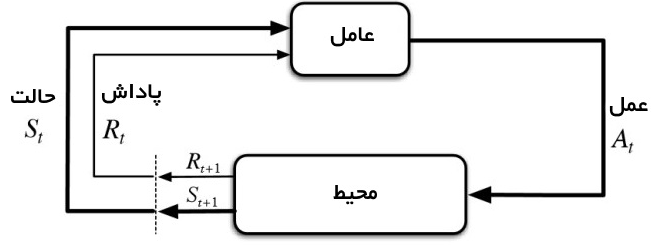
\includegraphics[scale=0.7]{./fig/rl}
  \caption{یادگیری تقویتی}
  \label{fig:rl}
\end{figure}
برخی از اصطلاحاتی که عناصر یک مساله یادگیری تقویتی را تشریح می‌کنند در ادامه بیان شده‌است.
\begin{itemize}
\item محیط (Environment):
 جهان فیزیکی که عامل در آن عمل می‌کند.
\item حالت (State):
 موقعیت کنونی عامل
\item پاداش (Reward):
 بازخورد از محیط
\item  سیاست (Policy):
 روشی برای نگاشت حالت عامل به عمل
\item  ارزش (Value):
 پاداش آینده که یک عامل با اقدام به یک عمل در یک حالت خاص به آن دست می‌یابد.
\end{itemize}
یادگیری تقویتی عمیق
DRL \LTRfootnote{Deep Reinforcement Learning}،
 از شبکه‌های عصبی عمیق برای حل مسائل یادگیری تقویتی استفاده می‌کند، از این رو در نام آن از کلمه عمیق استفاده شده‌است. با در نظر گرفتن Q-Learning که یادگیری تقویتی کلاسیک محسوب می‌شود و Deep-Q-Learning می‌توان تفاوت آن‌ها با یکدیگر را دید. در رویکرد اول، از الگوریتم‌های سنتی برای ساخت جدول Q استفاده می‌شود تا به عامل در یافتن اقدامی که باید در هر حالت انجام شود کمک کند. در دومین رویکرد، از شبکه عصبی (برای تخمین پاداش بر مبنای حالت: مقدار q) استفاده می‌شود.

در مقاله‌ی
 \cite{gan1, gan2}
سناریویی در نظر گرفته شده‌است که شامل چندین برش در یک شبکه دسترسی رادیویی با ایستگاههای پایه است که از منابع فیزیکی مشترک (به عنوان مثال، پهنای باند) استفاده میکنند. 
با استفاده از یادگیری تقویت عمیق (DRL) با در نظر گرفتن تقاضای مختلف خدمات به عنوان وضعیت محیط و منابع اختصاص یافته به عنوان عمل محیط، این مشکل حل می‌شود.
برای کاهش نویز و رسیدن به سطح انتظار خدمات، از روش GAN در بخش عمیق الگوریتم استفاده شده‌است که منجر به حداقل رساندن اختلاف بین توزیع مقدار-عمل تخمین زده شده و توزیع ارزش عمل هدف
می‌شود.
برای یافتن سیاست بهینه ی تخصیص منابع از روش
DDQN \LTRfootnote{Double Deep Q-Network}
 استفاده می‌شود.
\begin{figure}
  \centering
    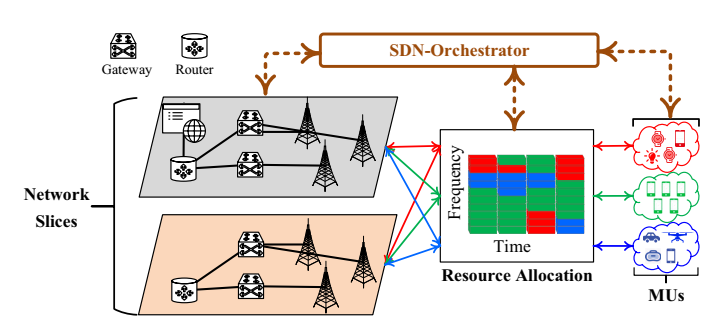
\includegraphics[scale=0.7]{./fig/gan}
  \caption{سناریوی ارسال لینک بالا و پایین در برشهای شبکه }
  \label{fig:gan}
\end{figure} 
 
در مقاله‌ی
\cite{li2020end} 
الگوریتم تخصیص منابع برش شبکه انتها به انتها مبتنی بر 
DQN \LTRfootnote{deep Q-Network}
 پیشنهاد شده‌است که برای سناریوهای چند برش و چند سرویس مناسب است.
 در این سیستم دو مدل سرویس ارائه شده‌است که اولی بر مبنای نیاز به رسیدن به نرخ خاص و دومی نیازمند داشتن تاخیر کم می‌باشد.
هدف در این سیستم رسیدن به بیشینه نرخ دسترسی است.
برای رسیدن به هدف مورد نظر برشها به دو بخش دسترسی و اصلی تقسیم شده‌اند.
 در اینجا الگوریتم به طور مشترک برشهای شبکه دسترسی رادیویی و برشهای شبکه اصلی را در نظر می‌گیرد تا منابع را به صورت دینامیکی طوری اختصاص دهد که 
 حداکثر میزان کاربران به شبکه دسترسی داشته و به بیشینه نرخ برسد.
 این سیستم به صورت برنامه ی
 mixed-integer
 نوشته می‌شود
و مسئله به صورت دو مسئله ی کوله پشتی و اتصال لینک ها بیان می‌شود
  و با استفاده از روش
 DQN
 حل می‌گردد.
 \subsection{مسائل امنیتی و تکنیک MTD}
تکنیک‌های ML، از جمله DRL، در برابر حملات خصمانه مختلف با هدف فریب دادن مدل ML به تصمیم‌گیری نادرست با تزریق یا دستکاری داده‌ها در طول مراحل (دوباره) آموزش یا ارائه مدل~\cite{aisecme} آسیب‌پذیر هستند.
به عنوان مثال، دستکاری در منابع واقعی موجود ممکن است باعث شود که یک مدل پذیرش برش مبتنی بر DRL درخواست‌های جدید برش RAN را به اشتباه رد کند. بنابراین، امنیت تکنیک های ML برای ادغام آنها با O-RAN حیاتی است و اعتماد را در تصمیمات آنها تقویت می کند.

یک اقدام دفاعی امیدوارکننده که در ~\cite{aisecme} ترویج می‌شود، پارادایم دفاع هدف متحرک (MTD) \LTRfootnote{Moving Target Defense} است که هدف آن افزایش عدم اطمینان مهاجم با تغییر مداوم و پویا سطح حمله در طول زمان است.
در واقع، MTD اخیراً به عنوان یک رویکرد مؤثر برای بهبود استحکام مدل‌های ML با تبدیل یک مدل به یک هدف متحرک در برابر حملات دشمن ظاهر شده است. قابل توجه است که بیشتر مشارکت‌ها بینایی رایانه و دامنه‌های بدافزار را هدف قرار می‌دهند (به عنوان مثال 
 ~\cite{sengupta2019mtdeep, rashid2022mtd}
 ).
در \cite{qiu2021mt}، نویسندگان یک چارچوب دفاعی حمله تروجانینگ را بر اساس یک MTD در شبکه عصبی عمیق (DNN) در نظر می‌گیرند، که به‌طور تصادفی ابعاد را در مدل‌های آموزشی چند بعدی انتخاب می‌کند. با توجه به نتایج، آنها در دسترس بودن DNN را تضمین کرده و از آن در برابر حملات تروجان محافظت می کنند.
 \section{نتیجه گیری}
 در این فصل، ابتدا در مورد مسائل پیشین صحبت می‌نماییم که شامل مسائل مرتبط با برش شبکه، شبکه‌های دسترسی رادیویی باز و قرارگیری توابع شبکه‌ی مجازی می‌باشد. سپس در مورد روشهای حل صجبت نمودیم. این روشها شامل دو مسئله‌ی NP-Hard است که مسئله‌ی کوله‌پشتی و بسته‌بندی جعبه را شامل می‌شود. همچنین روش حل دیگر، روش یادگیری تقویتی است که با استفاده از روشهای یادگیری ماشین به حل مسائل می‌پردازد. در انتها در مورد مسائل امنیتی در روشهای یادگیری ماشین صحبت نمودیم و مشکلات و راه حل های آن را مورد بررسی قرار دادیم.		% فصول دوم: مروری بر مطالعات انجام شده
\chapter{تخصیص منابع در شبکه‌های دسترسی رادیویی باز}
\section{مقدمه}
در اینحا هدف ما، فرمول بندی برش RAN برای معماری O-RAN است. این مطالعه، تکنیکی را برای ایجاد خطوط کلی برش شبکه ایزوله در معماری O-RAN برای ارائه QoS خاص برای eMBB، URLLC و mMTC ارائه می‌کند. علاوه بر منابع باند پایه، تعداد VNF ها نیز برای کاهش تأخیر به ویژه برای خدمات URLLC، در نظر گرفته می شود.
در این بخش هدف تخصیص منابع در ساختار شبکه های دسترسی رادیویی باز با استفاده از برش شبکه برای سرویسهای مختلف با کیفیت سرویس متفاوت باتوجه به شکل \ref{fig:c11} می باشد. 
خلاصه‌ی مهم‌ترین نوآوری‌های این بخش بدین صورت است:
\begin{itemize}
	\item 
	در اینجا یک مدل برش شبکه را برای سه سرویس مختلف معرفی شده در \lr{5G}، یعنی eMBB، mMTC و URLLC به تصویر می‌کشد. در معماری O-RAN، مشکل تخصیص منابع رادیویی و فعال سازی VNF بررسی می شود.
	ما بر اساس انواع مختلف خدمات با اولویت ها و QoS مختلف، یک مسئله برای تخصیص منابع باند پایه برای به حداکثر رساندن توان عملیاتی وزنی O-RAN فرموله می کنیم.
	\item 
	ما دراینجا تأخیر پردازش و منابع VNF مورد نیاز برای برش را در مقایسه با سایر مقالات در نظر گرفته‌ایم. بنابراین، ما بر به دست آوردن تعداد بهینه VNF در هر لایه از معماری O-RAN تمرکز می نماییم.
	همچنین سرویسهای مختلف با QoS مختلف شامل تاخیر، توان و نرخ را بررسی نموده‌ایم و با توجه به تعداد VNFهای فعال شده و نرخ هر کابر، تاخیر پردازشی انتها به انتها را بدست می‌اوریم.
	
	با فرض ظرفیت محدود فرانتهال، توان و ظرفیت واقعی هر O-RU را محاسبه می کنیم. بسته به نوع سرویس، تداخل O-RUهای همسایه را مدل کرده و نرخ را تعیین می‌نماییم. در مدل سیستم در نظر گرفته شده، انتقال بسته کوتاه URLLC و mMTC را به حساب می‌آوریم که نمی‌توان با قضیه ظرفیت شانون مدل‌سازی کرد.
\item 	
مسئله‌ی مورد بررسی، یک مسئله‌ی غیرخطی همراه با  ترکیب اعداد صحیح و پیوسته است که برای حل آن از یک الگوریتم دو مرحله‌ای تکراری استفاده می‌نماییم که در مرحله‌ی اول، تعداد VNFهای فعال، تخصیص توان و PRB بدست می‌آید و در مرحله‌ی دوم ارتباط کاربران با o-RU ها بدست می‌آید.
\item 
ما مسئله‌ی اصلی را در مرحله‌ی اول برای یافتن یک کران بالا و پایین برای تعداد VNF های فعال شده مجدداً فرموله و ساده می کنیم و از تابع لاگرانژی و شرایط KKT برای یافتن توان بهینه و تخصیص PRB استفاده می کنیم.
برای مرحله دوم، مسئله‌ی ارتباط O-RU را می توان به یک مسئله‌ی کوله پشتی چندگانه تبدیل کرد و با الگوریتم حریصانه حل کرد.
\item 
در نهایت، بحث در مورد انتخاب نقطه اولیه و منطقه امکان پذیر برای نتایج عددی ارائه شده است. همچنین، ما یک الگوریتم سریع را معرفی می‌کنیم که پیچیدگی کمتری نسبت به روش ما برای تحقق بخشیدن به منطقه امکان‌پذیر برای مسئله‌ی ما دارد. 
\end{itemize} 

\begin{figure}
  \centering
  \captionsetup{justification=centering}
    \includegraphics[scale = 0.4]{./img/finalDraw1.pdf}
    %\includegraphics[width=9.cm,height=6.2cm]{finalDraw1.pdf}
    %\includegraphics[width=\textwidth]{finalDraw.pdf}
  \caption{برش شبکه در سیستم O-RAN}
  \label{fig:c11}
\end{figure}
در ادامه‌ی این فصل، ابتدا مدل سیستم و فرمولاسیون مسئله را بیان می‌نماییم. سپس الگوریتم مورد نظر را ارائه داده و در نهایت     نتایج عددی رو بیان می کنیم.

\section{مدل سیستم و فرمولاسیون مسئله}\label{systemmodel}
در این بخش، سیستم فروسو \LTRfootnote{Downlink} را در معماری O-RAN با استفاده از برش RAN همانطور که در شکل \ref{fig:c11} نشان داده شده است، توصیف می کنیم.
ابتدا مدل سیستم را ارائه می کنیم. سپس، نرخ‌های داده قابل دستیابی، توان O-RU و ظرفیت فرانتهال برای لینک فروسو سیستم O-RAN را به دست می‌آوریم. پس از آن، میانگین تاخیر و توان VNF ها را مورد بحث قرار می دهیم.
در نهایت مسئله‌ی اصلی بیان می شود.
\subsection{مدل سیستم}
فرض کنید، سه نوع سرویس شامل eMBB، URLLC و mMTC وجود دارد که از برنامه های مختلف پشتیبانی می کنند.
بر این اساس، برش‌های $S_1$ برای نوع سرویس اول (eMBB)، برش‌های $S_2$ برای نوع سرویس دوم (URLLC) و برش‌های $S_3$ برای نوع سرویس سوم (mMTC) وجود دارد.

بنابراین،  $S$ برش‌ از پیش تخصیص داده شده وجود دارد که به این $S$ سرویس، خدمات ارائه می‌کنند ($S = S_1 + S_2 + S_3$).
بنابراین، هر درخواست سرویس $s\in \{1,\ldots,S\}$ توسط بخش مربوطه ارائه می‌شود.
بنابراین  $\{1,2,...,S_1\}$ 
مجموعه ای از نمونه‌های سرویس 
eMBB
می‌باشد. همچنین
 $\{1,2,...,S_2\}$ 
  مجموعه‌ای از نمونه‌های سرویس  URLLC
  است. 
   و $\{1 داریم. ,2,...,S_3\}$ مجموعه نمونه های سرویس mMTC می‌باشد.
   
   هر سرویس $s_j\in \{1,2,...,S_j\} $ شامل درخواست‌های $U_{s_j}$ از UE‌های تک آنتنی است که به سطح خاصی از QoS نیاز دارند.
   همچنین $j \in \{1,2,3\}$ نوع سرویس را نشان می‌دهد.
   درخواست های کاربردی مختلفی وجود دارد که در یکی از این دسته خدمات قرار می گیرند. هر درخواست برنامه به QoS خاصی نیاز دارد. بر اساس درخواست و QoS
   مورد نظر، 
    کاربر،
     ممکن است پذیرفته شده و به منابع اختصاص یابد.
   هر برش شبکه از پیش تخصیص داده شده حاوی VNF های رزرو شده برای سه گره منطقی است:
   
   
   \begin{itemize}
   	\item MAC/RLC در گره منطقی O-DU عمل می کند
   	\item PDCP/SDAP در گره منطقی O-CU-UP عمل می کند
   	\item گره منطقی UPF
   \end{itemize}
   
   هر تکه $s \in \{1,2,...,S \}$، شامل $M_s^{d}$ VNF برای پردازش O-DU،   
   $M_s^c$
   VNF 
   برای O-CU-UP و 
   $M_s^u$
   تا VNF 
   برای UPF می‌باشد.
   VNFهای O-DU، O-CU-UP و UPF به هم متصل هستند، که به عنوان زنجیره عملکرد سرویس (SFC) در سیستم O-RAN تعریف شده است. همچنین، هر نمونه VNF روی یک ماشین مجازی (VM) اجرا می شود که از منابع مراکز داده استفاده می کند.
   
   فرض کنید در این سیستم K بلوک‌ منبع فیزیکی (PRB)
     وجود دارد.
   
   فرض کنید هر برش $s$ متشکل از $\bar{K}_s$ بلوک های منبع مجازی از پیش تخصیص یافته است که به بلوک های منابع فیزیکی (PRB) نگاشت شده اند. بنابراین، $\sum_s \bar{K}_s \leq K$ داریم.
   علاوه بر این، R تا
    O-RU های چند آنتنی وجود دارد که بین برش ها مشترک هستند.
   O-RU $r \in \{1,2,...,R \}$ دارای آنتن $J$ برای انتقال و دریافت داده است. همچنین $\mathcal{R} = \{ r \ | \ r\in 1,2,...,R \}$ مجموعه ای از O-RU ها را نشان می دهد. علاوه بر این، همه O-RU ها به همه PRB ها دسترسی دارند.
 \subsection{مدل سیگنال}
   اگر گیرنده $i$ در سرویس $s$ را در نظر بگیرید، سیگنال دریافتی $y_{u(s,i)}$ به صورت زیر تعریف می‌شود:
   
   \begin{equation}\label{eq2}
   	y_{u(s,i)} = \sum_{r=1}^{R} \sum_{k=1}^{K_s} \boldsymbol{h}^{H \: k}{r,u(s,i)} g{u(s,i)}^r e^k_{r,u(s,i)}{x_Q}^k_{r,u(s,i)} + z_{u(s,i)}
   \end{equation}
   
   در این معادله، ${x_Q}^k_{r,u(s,i)} = {x_P}^k_{r,u(s,i)} + \boldsymbol{q}_{r}$ است. همچنین ${x_P}^k{r,u(s,i)} = \boldsymbol{w}^k_{r,u(s,i)}\sqrt{p^{k}{r,u(s,i)}} x{u(s,i)}$ و $x_{u(s,i)}$ بردار نمادهای فرستاده شده را نشان می‌دهد. همچنین $z_{u(s,i)} \sim \mathcal{CN}(0,BN_0)$ نویز گاوسی افزایشی دریافت را نشان می‌دهد که $BN_0$ توان نویز در یک پهنای باند مشخص است. در اینجا، ${x_P}$ پیام پیشکدشده قبل از فشرده‌سازی را نشان می‌دهد، در حالی که ${x_Q}$ پیام پیشکدشده پس از فشرده‌سازی است. 
   
   علاوه بر این، $\boldsymbol{q}{r} \sim \mathcal{CN}(0,{\sigma_q}^2\boldsymbol{I{R}} )$ نویز گاوسی کوانتیزاسیون را نشان می‌دهد که از فشرده‌سازی سیگنال در O-DU ناشی می‌شود. همچنین، $g_{u(s,i)}^r \in \{0,1\}$ متغیر دودویی است که نشان می‌دهد که آیا O-RU $r$ به خدمتگیری $i$ که به تخصیص به تکه $s$ است، خدمت می‌دهد یا خیر. علاوه بر این، $p_{r,u(s,i)}^{k}$ توان انتقال O-RU $r$ به خدمتگیری $i$ در تکه $s$ و PRB $k$ را نشان می‌دهد، در حالی که ${\bold{h}_{r,u(s,i)}^{k}} \in \mathbb{  	C}^{J}$ بردار کانال مربوطه است. همچنین، $\bold{w}_{r,u(s,i)}^{k} \in \mathbb{C}^{J}$ بردار پرتاب‌نور فرستنده مربوطه را نشان می‌دهد.
   
   با توجه به \eqref{eq1}، SINR خدمتگیری $i$ ام در تکه $s$ بر روی PRB $k$ به صورت زیر محاسبه می‌شود:
   
   \begin{equation}\label{eq1}
   	\rho_{r,u(s,i)}^{k} = \frac{p_{r,u(s,i)}^{k}|{\bold{h}{r,u(s,i)}^{k \: H}} \bold{w}{r,u(s,i)}^{k}|^2}{BN_0 + I_{r,u(s,i)}^{k}}
   \end{equation}
   
   یک UE در O-RU $r$ با استفاده از PRB $k$ تداخل از سایر O-RUهای موجود در مجموعه $\mathcal{R}\backslash r$ که از PRB $k$ استفاده می‌کنند، دریافت می‌کند. دو نوع تداخل بین UEها در هر تکه وجود دارد: i- تداخل بین تکه‌ها (inter-slice) که از طریق سیگنال‌هایی که از تکه‌های مختلف فرستاده می‌شوند، و ii- تداخل درون تکه (intra-slice) که از طریق سیگنال‌هایی که در یک تکه فرستاده می‌شوند، رخ می‌دهد.
   
   تکنیک‌های شکستن شبکه
   \LTRfootnote{network slicing} 
   تداخل بین سرویس‌ها را به طور قابل توجهی کاهش می‌دهند. یک روش برای استفاده از زمان‌بندی PRB دو مقیاسی، مجزا کردن PRBها در تکه‌ها (در مقیاس زمانی اول) و برنامه‌ریزی PRBها برای UEهای برشها (در مقیاس زمانی دوم) است. یک روش دیگر شامل اختصاص بخشی از PRBهای سرویس‌های eMBB به URLLC و mMTC است.
  \cite{alsenwi2021intelligent, setayesh2020joint, mei2021intelligent}. در این مقاله، فرض می‌کنیم که زمان‌بندی PRB انجام شده است. همچنین، در بخش \ref{prb}، به طور خلاصه برنامه‌ریزی PRB بین برشها را مورد مطالعه قرار می‌دهیم.
  از آنجا که منابع محدود هستند، تداخل بین سرویس‌ها به طور کامل قابل حذف نیست. با این حال، جدا کردن برشها تداخل بین سرویس‌ها را به طور قابل توجهی کاهش می‌دهد و می‌توانیم در محاسبات ریاضی به آن توجه نکنیم.
  بازگشت به \eqref{eq1}، $I_{r,u(s,i)}^{k}$ مجموع قدرت سیگنال‌های مزاحم و نویز کوانتیزاسیون است و می‌تواند به صورت زیر نمایش داده شود:
\begin{align}\label{eqI}
	&I_{r,u(s,i)}^{k} =\underbrace{  \sum_{j=1}^{{R}} {\sigma_q}^2 |\boldsymbol{h}_{r,{u(s,i)}}^k|^2 }_{\text{(quantization noise)}} + \nonumber\\
	&\underbrace{\sum_{\substack{l=1 \\ l\neq i}}^{{U}_{s}}\! e^{k}_{u(s,i)}e^{k}_{u(s,l)}  p_{u(s,l)}^{k}\!\!\sum_{\substack{r'=1 \\ r'\neq r}}^{R}\!|{\bold{h}_{r',u(s,i)}^{k \: H}} \bold{w}_{r',u(s,l)}^{k} g_{u(s,l)}^{r'}|^2}_{\text{(intra-slice interference)}},
\end{align}
  که $e^{k}_{u(s,i)}$ یک متغیر دودویی است که نشان می‌دهد آیا PRB $k$ به UE $i$ در تکه $s$، که به O-RU $r$ تخصیص داده شده است یا نه. همچنین، هیچ تداخل بین برشهاوجود ندارد، فقط تداخل درون برشها، از آنجا که فرض می‌شود تکه‌ها جداگانه هستند.
  در اینجا، بردار پرتاب‌نور صفر نیرو (zero-forcing) مورد استفاده قرار می‌گیرد که تداخل درون تکه را به حداقل می‌رساند و به صورت زیر تعریف می‌شود:
\begin{equation}
	\bold{w}_{r,u(s,i)}^{k} = \hat{\bold{h}}_{r,u(s,i)}^{k}(\hat{\bold{h}}_{r,u(s,i)}^{k \: H} \hat{\bold{h}}_{r,u(s,i)}^{k})^{-1}.
\end{equation}
  برای محاسبه SINR برای سرویس $s$ در UE $i$ می‌توان از \eqref{eqI} و \eqref{eqW} استفاده کرد. در نهایت، با استفاده از SINR، می‌توان میزان داده‌های دریافتی $i$ را محاسبه کرد. 
   
   \subsection{نرخ انتقال داده}

   نرخ داده قابل دستیابی برای درخواست مورد نظر $i$امین کاربر در برنامه $s_1$ام از نوع سرویس 1 (eMBB) را می‌توان به شکل زیر نمایش داد:
   \begin{equation}\label{eq3}
   	\mathcal{R}_{u(s_1,i)} = \sum_{r=1}^{R}\mathcal{R}_{r,u(s_1,i)} g^r_{u(s_1,i)},
   \end{equation}
   که در آن:
   \begin{equation}
   	\mathcal{R}_{r,u(s_1,i)} = \sum_{k=1}^{K} \mathcal{{R}}_{r,u(s_1,i)}^{k} e^k_{r,u(s_1,i)}
   \end{equation}
   نرخ داده قابل دستیابی برای RU $r$ به UE $i$ در برش $s_1$ است که وابسته به نرخ داده قابل دستیابی در هر PRB می‌باشد و به شرح زیر تعریف می‌شود:
   \begin{equation}
   	\mathcal{{R}}_{r,u(s_1,i)}^{k} =  B \log_2({1+ \rho_{r,u(s_1,i)}^{k}}),
   \end{equation}
   از آنجا که طول بلوک در URLLC و mMTC محدود است، نرخ داده قابل دستیابی برای درخواست $i$امین کاربر در برنامه سرویس 2 (URLLC) و 3 (mMTC) از فرمول ظرفیت شانون بدست نمی‌آید. به جای آن، در انتقال بسته‌های کوتاه، نرخ داده قابل دستیابی به شکل تقریبی محاسبه می‌شود \cite{setayesh2020joint}:
   \begin{equation}\label{eq11}
   	\mathcal{R}_{u(s_j,i)} = \sum_{r=1}^{R}\mathcal{R}_{u(s_j,i)}^{r} g^r_{u(s_j,i)},
   \end{equation}
   که در آن:
   \begin{equation}
   	\mathcal{R}_{r,u(s_j,i)} = \mathcal{{R}}_{r,u(s_j,i)}^{k}{e}_{u(s_j,i)}^{k},
   \end{equation}
   نرخ داده قابل دستیابی برای RU $r$ به UE $i$ در برش $s_j$ است که وابسته به نرخ داده قابل دستیابی در هر PRB می‌باشد و به شرح زیر تعریف می‌شود:
   \begin{equation}
   	\mathcal{{R}}_{r,u(s_j,i)}^{k} = B \log_2({1+ \rho_{r,u(s_j,i)}^{k}} - \zeta_{u(s_j,i)}^{k}){e}_{u(s_j,i)}^{k},
   \end{equation}
   به طوری که:
   \begin{equation}\label{shortPacket}
   	\zeta_{u(s_j,i)}^{k} = \log_2({e})Q^{-1}(\epsilon) \sqrt{\mathfrak{C}_{u(s_j,i)}^{k}/N_{u(s_j,i)}^{k}}.
   \end{equation}
در اینجا، $\epsilon$ احتمال خطا در انتقال است، $Q^{-1}$ معکوس تابع Q است، 
$\mathfrak{C}_{u(s_j,i)}^{k} = 1 - \frac{1}{(1+\rho_{u(s_j,i)}^{k})^2}$، پراکندگی کانال کاربر $i$ در برش $s_j$ و PRB $k$ را نشان می‌دهد، در حالی که
$N_{u(s_j,i)}^{k}$ طول بلوک انتقال متناظر را نمایش می‌دهد.
$\mathcal{R}_{r,u(s_j,i)}$ نرخ داده قابل دستیابی است که توسط O-RU $r$ به کاربر $i$ که درخواست سرویس $s_j$ را دارد، انتقال داده می‌شود.

اگر در رابطه \eqref{eqI} مقادیر $p_{u(s,l)}^{k}$ و $p_{u(n,l)}^{k}$ را با $P_{s}^{\text{max}}$ جایگزین کنیم، برای $I_{r,u(s,i)}^{k}$ یک مرز بالا $\bar{I}_{r,u(s,i)}^{k}$ بدست می‌آید. بنابراین، با استفاده از $\bar{I}_{r,u(s,i)}^{k}$ به جای $I_{r,u(s,i)}^{k}$ در روابط \eqref{eq11} و \eqref{eq3}، $\bar{\mathcal{R}}_{u_{(s,i)}} \forall s , i$ بدست می‌آید.

\subsection{توان O-RU و ظرفیت Fronthaul}
مجموعه توان ارسالی سیگنال از O-RU $r$ام به تمامی کاربرانی که توسط آن خدمت داده می‌شوند را با $P_r$ نشان می‌دهیم. از رابطه \eqref{eq2}، توان هر O-RU $r$ به صورت زیر بدست می‌آید:
\begin{equation}\label{pr}
	P_r = \sum_{s=1}^{S}\sum_{k=1}^{K_s}\sum_{i=1}^{U_s}|\bold{w}_{r,u(s,i)}^{k}|^2\alpha^k_{r,u(s,i)} + \sigma_{q}^2,
\end{equation}
که در آن $\alpha^k_{r,u(s,i)}= p_{r,u(s,i)}^{k} g_{u(s,i)}^r e^k_{r,u(s,i)}$ است.
از آنجا که یک پیوند فیبر بین O-RU و O-DU وجود دارد،

ظرفیت ارتباطی کاربران در پیوند ارتباطی (fronthaul) بین O-DU و O-RU $r$ام به صورت زیر تعریف می‌شود:
\begin{align}\label{cr}
	C_{r} &= \log_2{\left(1+ \sum_{s=1}^{S}\sum_{k=1}^{K_s}\sum_{i=1}^{U_s}|\bold{w}_{r,u(s,i)}^{k}|^2 \mathcal{\alpha}^k_{r,u(s,i)} / \sigma_{q}^2\right)}\nonumber\\
	&= \log_2{\left(P_r/\sigma_{q}^2\right)}.
\end{align}
\subsection{میانگین تاخیر}
در این بخش، تاخیر میانگین انتها به انتهای هر سرویس به دست می‌آید. تاخیر کل ($T^{\text{\text{tot}}}$) مجموع تاخیر پردازش ($T^{\text{proc}}$)، تاخیر انتقال ($T^{tr}$) و تاخیر کل پخش ($T^{\text{pro}}$) است.
\begin{subequations}
	\begin{alignat}{4}
		T^{\text{\text{tot}}} &=  T^{\text{proc}} + T^{tr} + T^{\text{pro}},\\
		T^{\text{\text{proc}}} &=  T^{\text{RU}} + T^{\text{DU}} + T^{\text{CU}} + T^{\text{UPF}},\\
		T^{\text{tr}} &= T^{\text{fr},t} + T^{\text{mid},t} + T^{\text{b},t},  \\
		T^{\text{pro}} &= T^{\text{fr},p} + T^{\text{mid},p} + T^{b,p}.
	\end{alignat}
\end{subequations}
%{\color{red} I made a mistake and replaced pro with proc. Please correct them. Also, explain in more details the processing delay in this paragraph.}
%T_{\text{\text{tot}}} = T_{RU} + T_{front} + T_{DU} + T_{\text{mid}} + T_{CU} + T_{back} + T_{core} + T_{trans2net}
بطور ریاضی، تاخیر کل پخش ($T^{\text{pro}}$) مجموع تاخیر پخش در لینک فرانت‌هاول ($T^{fr,p}$)، لینک مید‌هاول ($T^{\text{mid},p}$) و لینک بک‌هاول ($T^{b,p}$) است. در هر لینک، تاخیر پخش زمانی است که یک سیگنال برای رسیدن به مقصد خود طی می‌کند. این تاخیر بر اساس طول لینک فیبر و ظرفیت لینک (به عنوان $\text{T} = \text{L}/\text{c}$، که در آن L طول لینک و c سرعت پخش در وسط است) به دست می‌آید.
در عین حال، تاخیر کل انتقال ($T^{tr}$) مجموع تاخیر انتقال در فرانت‌هاول ($T^{fr,t}$)، مید‌هاول ($T^{\text{mid},t}$) و بک‌هاول ($T^{b,t}$) است.
در هر لینک، تاخیر انتقال زمانی است که برای فشرده‌سازی تمام بسته

‌ها به محیط انتقال نیاز است و می‌توان آن را به صورت $T = \frac{\mathcal{\alpha}}{R}$ فرمول‌بندی کرد، جایی که R نرخ داده بسته و $\mathcal{\alpha}$ اندازه میانگین بسته است.
توجه کنید که در نظر گرفتن تاخیر پخش و انتقال در فرمول‌بندی به راحتی قابل انجام است، اما ما به دلایل خلاصه‌سازی و سادگی از آن پرهیز کرده‌ایم.
%می‌تواند منجر به یک فرمول‌بندی مسئله جدید شود که می‌تواند به مدل سیستم ما اضافه شود تا در آینده کار را گسترش دهد. در مقاله کنونی، فرض می‌کنیم که اتصال بین O-RU و O-DU ثابت و شفاف است و مشکل پردازش لبه را مد نظر قرار نمی‌دهیم.
بنابراین، تاخیر پخش ثابت است و تأثیری در مسئله بهینه‌سازی ندارد.

سپس، محاسبه مختصری از تاخیر انتقال ارائه می‌دهیم تا نشان دهیم که مشارکت آن در تاخیر کل بی‌اثر و بر بهینه‌سازی تأثیری ندارد.
در URLLC و mMTC، اندازه میانگین بسته ممکن است بین 20 تا 32 بایت باشد، در حالی که حداقل نرخ داده را به عنوان $1\ \text{bps/Hz} \times \text{BW (180 KHz)}$ در نظر می‌گیریم. بنابراین، تاخیر انتقال از O-RU به O-DU حدوداً $T^{fr,t} = \frac{20\times 8}{1 \times 180 \times 10^3} < 0.1\ \text{ms}$ و $T^{fr,t} \approx T^{mid,t} \approx T^{b,t}$ است. برای eMBB، اندازه بسته ممکن است 100 برابر بزرگتر باشد و تاخیر آن بیش از 0.6 میلی‌ثانیه نمی‌شود.
بنابراین، در ادامه،

فرض می‌کنیم که تاخیر کل تقریباً برابر با تاخیر پردازش است ($T^{\text{\text{tot}}} \approx T^{\text{proc}}$).


\subsubsection{تاخیر پردازشی}

فرض می‌کنیم ورودی بسته‌های کاربران (UE) با فرآیند پوآسون با نرخ $\lambda_{u(s,i)}$ برای کاربر $i$ام سرویس $s$ام اتفاق می‌افتد. بنابراین، نرخ متوسط ورود داده در لایه UPF برای سلیس $s$ام برابر است با $\alpha_{s}^U = \sum_{u=1}^{U_s}\lambda_{u(s,i)}$.
همچنین، فرض می‌کنیم که نرخ متوسط ورود داده در لایه UPF برای سلیس $s$ام ($\alpha_{s}^U$) تقریباً برابر است با نرخ متوسط ورود داده در لایه O-CU-UP ($\alpha_{s}^C$) و O-DU ($\alpha_{s}^D$)، به عبارت دیگر $\alpha_{s} =\alpha_{s}^U \approx \alpha_{s}^C \approx \alpha_{s}^D$. این امر به این دلیل است که مقدار داده‌های منتقل شده در طول مسیر (بدون توجه به تغییرات فریم) ثابت است.
در واقع، طبق قضیه Burke، نرخ متوسط ورود داده در لایه‌های دوم و سوم که در لایه اول پردازش می‌شوند، همچنان با نرخ $\alpha_{s}$ پوآسون است.
فرض می‌کنیم در هر لایه برای هر سرویس باربندگانی وجود دارد تا ترافیک ورودی را به صورت مساوی بین VNFها تقسیم کنند.
فرض می‌کنیم پردازش پایه‌ای هر VNF به وسیله یک صف پردازش M/M/1 مدل می‌شود.
زیرا بسته‌های ورودی سیستم از منابع مستقل بسیاری می‌آیند. علاوه بر این، تأثیر یک بسته تکی بر عملکرد سیستم کم است. همچنین، روش صف به صورت FIFO است و فرض می‌کنیم که بسته ورودی فرآیند پوآسون را دنبال می‌کند. بنابراین، فرض می‌کنیم که زم

ان‌های سرویس از توزیع نمایی پیروی می‌کنند. به علاوه، از آنجایی که سرویس‌ها مستقل هستند، کاربران در هر سرویس اولویت یکسانی دارند و تأخیرهای پردازش هر سرویس مستقل از سرویس‌های دیگر است. بنابراین، یک سرویس ممکن است اولویت بالاتری داشته باشد که بر بهینه‌سازی کلی تأثیر می‌گذارد و تئوری صف M/M/1 همچنان اعتبار دارد.
هر بسته توسط یکی از VNFهای سلیس مربوطه پردازش می‌شود. بنابراین، تأخیر متوسط برای سلیس $s$ام در O-DU، O-CU و UPF به صورت صف پردازش M/M/1 مدل می‌شود و می‌تواند به شرح زیر باشد:

\[T_{s}^{\text{DU}} = \frac{1}{\mu_s^d - \frac{\alpha_{s}}{M_s^{d}}},\]

\[T_{s}^{\text{CU}} = \frac{1}{\mu_s^c - \frac{\alpha_{s}}{M_s^{c}}},\]

\[T_{s}^{\text{UPF}} = \frac{1}{\mu_s^u - \frac{\alpha_{s}}{M_s^{u}}},\]

که $M_s^{d}$، $M_s^{c}$ و $M_s^{u}$ به ترتیب تعداد VNFها در O-DU، O-CU-UP و UPF را نشان می‌دهند.
علاوه بر این، $1/\mu_s^d$، $1/\mu_s^c$ و $1/\mu_s^u$ زمان سرویس متوسط لایه O-DU، O-CU و UPF را نشان می‌دهند. نرخ ورود هر VNF برای هر سلیس $s$ام برابر است با $\alpha_{s}/{M_s^{i}}$، که $i \in \{d,c,u\}$ است.
در عین حال، نرخ ورودی داده برای هر UE $i$ از سرویس $s$ برابر $\lambda_{u(s,i)}$ است، بنابراین $\sum_{i = 1}^{U_s} \lambda_{u(s,i)} = \alpha_s$.
علاوه بر این، زمان سرویس دهی صف انتقال برای UE $i$ که درخواست سرویس $s$ را دارد، از توزیع نمایی با میانگین $1/R_{u(s,i)}$ پیروی می‌کند و می‌توان آن را به صورت صف M/M/1 مدل کرد \cite{SystemCostMinimization,luong2018joint,luong2018novel}.
بنابراین، تأخیر متوسط لایه انتقال برای UE $i$ در سلیس $s$ به شرح زیر است:

\[ T_{u(s,i)}^{\text{RU}} = \frac{1}{R_{u(s,i)} - \lambda_{u(s,i)}}.\]

ما فرض می‌کنیم $T^{\text{\text{tot}}}_{u(s,i)} \approx T^{\text{proc}}_{u(s,i)} $.
\subsection{توان VNF}
فرض می‌کنیم مصرف انرژی هر VNF در هر گره منطقی (O-DU، O-CU و UPF) در سرویس $s$ به ترتیب با $\phi_{s}^d$، $\phi_{s}^c$ و $\phi_{s}^u$ نمایش داده می‌شود.
بنابراین، هزینه کل سیستم برق مصرفی تمامی برش‌ها را می‌توان به صورت $\phi_{\text{\text{tot}}} = \sum_{s=1}^{S}\phi_{s}$ نشان داد.
یعنی $\phi_{s}$ از رابطه $\phi_{s} = M_s^u \phi_s^u + M_s^c \phi_s^c+ M_s^d \phi_s^d$ به دست می‌آید.

یکی از مسائل مهمی که در صنعت وجود دارد، کاهش مصرف انرژی است. مراکز داده از جمله مصرف کنندگان اصلی انرژی هستند. به علاوه، محدودیت‌هایی برای مصرف انرژی مراکز داده از جمله ماشین‌های مجازی (VMs) وجود دارد. بنابراین، یکی از اهداف ما، محدود کردن مصرف انرژی کل VNF‌ها که به صورت VM در مراکز داده اجرا می‌شوند، است. با اعمال یک سیاست سفارشی بر مصرف کلی انرژی، می‌توانیم مصرف انرژی مراکز داده را کنترل کنیم ($\phi^{\text{\text{tot}}} \leq \phi^{\text{max}}$).
\subsection{بیان مسأله}\label{prS}
فرض می‌کنیم برش $s$ (که به سرویس $s$ اختصاص داده شده است) یک عامل اولویت $\delta_s$ دارد (بر اساس اولویت سرویس میزبانی آن) به طوری که $\sum_{s=1}^S \delta_s =1$.
عامل اولویت هر برش بر اساس توافق سطح خدمات بدست می‌آید تا عدالت در سیستم ترویج یابد.
%\textcolor{red}{توضیح دهید چرا عامل اولویت را معرفی می‌کنید.}
هدف این مقاله بیشینه کردن مجموع نرخ تمامی UEs با محدودیت‌های QoS است که به شرح زیر است: 
\begin{subequations}\label{problem}
	\begin{alignat}{4}
		\max\limits_{\boldsymbol{P}, \boldsymbol{E}, \boldsymbol{M}, \boldsymbol{G} }   \quad &  \sum_{s=1}^{S}\sum_{i=1}^{U_s}\delta_s \bar{\mathcal{R}}_{u_{(s,i)}} \ \\
		\text{subject to} \quad  &  P_r \leq P^{\text{max}}_{r} \quad \forall r,
		\label{c11} \\
		&p_{r,u(s,i)}^{k}  \geq 0  \quad \forall i, r, s, k,\label{c12} \\
		&p_{r,u(s,i)}^{k}  \leq P_{s}^{\text{max}}  \quad \forall i, r, s, k,\label{c12-1} \\
		&\bar{\mathcal{R}}_{u_{(s,i)}} \geq \mathcal{R}_{{s}}^{\min} \quad \forall s, \label{c13} \\
		%&\mathcal{R}_{u_{(s_2,i)}}^u \geq  \mathcal{R}_{min}^{s_2,u} \quad \forall s_2, \label{c14} \\
		& C_r \leq C^{\text{max}}_r \quad \forall r, \label{c15}\\
		&T^{\text{\text{tot}}}_{u(s,i)}  \leq T^{\text{max}}_{s} \quad \forall i, s,\label{c16} \\
		& \mu_s \geq \alpha_s/M_s \quad \forall s,\label{c16-1} \\
		& \bar{\mathcal{R}}_{u_{(s,i)}} \geq {\lambda}_{u_{(s,i)}} \quad \forall i, s,\label{c16-2} \\
		& 0 \leq M_s \leq M^{\text{max}}_s  \quad \forall s,\label{c16-3}\\
		& \phi^{\text{\text{tot}}}  \leq \phi^{\text{max}}, \label{c19} \\
		%& P_r\{E_1, E_2, E_3, E_4\} \leq \epsilon_s \quad \forall s_2, \label{c166}\\
		& \sum\nolimits_{\forall r}g^r_{u(s,i)} = 1  \quad \forall s, i, \label{c17}  \\
		& \sum_{k =1}^{K_s} g^r_{u(s,i)} e^{k}_{r,u(s,i)} \geq 1  \quad \forall s, i , r, \label{c18-1} \\
		& \sum_{s =1}^{S}\sum_{i=1}^{U_s}g^r_{u(s,i)} e^{k}_{r,u(s,i)} \leq 1  \quad \forall s, i , r, \label{c18} \\
		& g^r_{u(s,i)} \in \{0,1\} \quad \forall s, i, \label{c20}  \\
		& e^k_{r,u(s,i)} \in \{0,1\} \quad \forall s, i. \label{c21}
	\end{alignat}
	\label{constraints}
\end{subequations}
در اینجا، $\bar{\mathcal{R}}{u{(s,i)}}$ با استفاده از $\bar{I}{r,u(s,i)}^{k}$ به جای $I{r,u(s,i)}^{k}$ در \eqref{eq11} و \eqref{eq3} بدست می‌آید.
 $\boldsymbol{P} =[p_{r,u(s,i)}^{k}], \:\: \forall s , i, r, k $، ماتریس چهاربعدی (4D) قدرت برای UEs است، $\boldsymbol{E} =[e_{r,u(s,i)}^k], \:\: \forall s , i, r, k$، نشان‌دهنده ماتریس دودویی چهاربعدی برای انتساب PRB است. علاوه بر این، $\boldsymbol{G} =[g_{u(s,i)}^r], \:\: \forall s , i, r$، ماتریس سه‌بعدی دودویی (3D) برای انتساب O-RU است. همچنین، $M = [M_s^d, M_s^c, M_s^u], \:\: \forall s$، ماتریسی است که تعداد VNF‌ها در هر لایه از برش را در بر می‌گیرد. توجه کنید که
\eqref{c11}، \eqref{c12} و \eqref{c12-1} قدرت هر O-RU و UE را محدود می‌کنند.
همچنین، \eqref{c13} نرخ هر UE درخواستی برای هر نوع سروی

س، به عنوان مثال eMBB، mMTC و URLLC، را بیشتر از یک آستانه محدود می‌کند. در عین حال،
\eqref{c15} و \eqref{c16} ظرفیت فرانت‌هال محدود و تاخیر نهایی از سیگنال دریافتی را نشان می‌دهند.
\eqref{c16-1} و \eqref{c16-2} به پایداری صف M/M/1 مربوط هستند،
\eqref{c16-3} تعداد VNF‌ها در هر برش را به دلیل منابع محدود محدود می‌کند، در حالی که
%\eqref{c16} شرطی است که تاخیر در هر لایه باید کمتر از آستانه باشد.
\eqref{c17} و \eqref{c18-1} تضمین می‌کنند که O-RU و PRB با UE مرتبط شوند.
همچنین، \eqref{c18} مطمئن می‌شود که هر PRB نمی‌تواند به بیش از یک UE مرتبط با همان O-RU اختصاص داده شود، \eqref{c19} نشان می‌دهد که هزینه ثابت انرژی VNF‌ها در هر برش از آستانه بیشتر نشود، در حالی که \eqref{c20} و \eqref{c21} محدودیت‌های ماتریس‌های دودویی $\boldsymbol{E}$ و $\boldsymbol{G}$ را تعیین می‌کنند.

\subsubsection{تخصیص PRB}\label{prb}
در این بخش، یک مطالعه مختصر در مورد مسئله زمان‌بندی PRB ارائه می‌دهیم که می‌تواند در دو مرحله تکمیل شود تا تداخل بین برش‌ها را حذف کرده و جداسازی برش‌ها را تضمین کند \cite{marabissi2019highly}.
اولین مرحله اختصاص PRB به برش‌ها است و دومین مرحله اختصاص PRB برش‌ها به UEs است که تعداد بهینه‌ی VNF‌ها را برای هر برش پیدا می‌کند، توان UEs را تخصیص می‌دهد و O-RU را به UEs اختصاص می‌دهد که از الگوریتم پیشنهادی \ref{proAlg} استفاده می‌کند.
فرض کنید $\mathcal{R}{{s}}^{\min}$ و $\mathcal{R}{{s}}^{\text{max}}$ نرخ داده حداقل و حداکثر هر UE در برش s باشد.
ابتدا باید تعداد میانگین PRB مورد استفاده توسط UEs در هر سرویس را پیدا کنیم. اگرچه mMTC و URLLC به طور معمول انتقال بسته‌های کوتاهی را می‌طلبند، اما هر UE در mMTC و URLLC نیاز به 1 PRB دارد. بنابراین، اگر برش s خدمات mMTC یا URLLC را ارائه دهد و با $U_s$ UEs در این برش، نیاز به $K_s = U_s \times 1$ PRB است. برای eMBB، فرض کنید نرخ میانگین هر UE در برش s که به UEs eMBB خدمت می‌کند، $\bar{R}_s = B\log_2(1 + \bar{\rho_s})$ باشد، جایی که $\bar{\rho_s}$ میانگین SINR UEs در برش s است.
بنابراین، حداقل تعداد PRB مورد نیاز برش s با $U_s$ UEs برابر است با $K_s^{\min} = \lceil{U_s \times \frac{\bar{R}s}{\mathcal{R}{{s}}^{\text{max}}}}\rceil$. همچن

ین، حداکثر تعداد PRB مورد نیاز برش s با $U_s$ UEs برابر است با $K_s^{\text{max}} = \lceil{U_s \times \frac{\bar{R}s}{\mathcal{R}{{s}}^{\min}}}\rceil$. همچنین، $K_s = (K_s^{\min}+K_s^{\text{max}})/2$ تعداد میانگین PRB مورد نیاز در برش s است.
هدف ما به دست آوردن تعداد PRB اختصاص داده شده به هر برش $s$ ($\bar{K_s}$) با حل مسئله زیر است:
\begin{subequations}\label{prob:prb}
	\begin{alignat}{4}
		\max\limits_{\boldsymbol{\bar{K_s}}} \quad &  \sum_{s=1}^{S}\delta_s K_s \ln(\bar{K_s}) \ \\
		\text{محدودیت} \quad  & \sum_s{\bar{K_s}} \leq K
		\label{prb0}, \\
		& K_s^{\min} \leq \bar{K_s}  \leq K_s^{\text{max}}  \quad \forall s \in S_1,\label{prb1} \\
		&  \bar{K_s} \leq K_s  \quad \forall s \in S_2, S_3.\label{prb2}
	\end{alignat}
	\label{constraints}
\end{subequations}
برای اختصاص PRB به تمام برش‌ها از لگاریتم استفاده می‌کنیم تا آن‌ها را به‌صورت مساوی عادلانه کنیم، زیرا عدالت نسبی توسط بیشینه کردن تابع خودیت لگاریتمی دست‌یافته می‌شود \cite{marabissi2019highly}.
معادله \eqref{prb0} نشان می‌دهد که مجموع PRB برش‌ها نباید از حداکثر تعداد PRB ($K$) بیشتر شود.
معادله \eqref{prb1} تعداد PRB برش‌های eMBB را محدود می‌کند و \eqref{prb2} تعداد PRB برش‌های URLLC و mMTC را محدود می‌کند. با تساعد $\bar{K_s}$، تابع هدف و محدودیت‌ها به صورت محدب تبدیل می‌شوند و می‌توان با استفاده از تابع لاگرانژین آن‌

ها را حل کرد.

\subsubsection{مدیریت برش شبکه}		% فصل سوم: روش تحقیق
\chapter{تخصیص برش شبکه به صورت دینامیکی}
\section{مقدمه}
در این فصل هدف تخصیص برش شبکه به صورت دینامیکی می‌باشد. در فصل قبلی مدل سیستم به طور کامل نوشته شده است و در حالت آفلاین حل گردیده است، در این فصل پارامترها مورد نیاز را نسبت به فصل قبلی کمتر کرده و با استفاده از روش دینامیکی در هر لحظه از زمان به حل سیستم می‌پردازیم. برای حل این سیستم از روش یادگیری تقویتی استفاده می‌کنیم.
در بخش اول صورت مسئله‌ی بخش رادیویی نوشته می‌شود. سپس  به مدل سیستم بخش هسته می‌پردازیم و در نهایت روش حل هر دو مسئله و نتایج عددی آن بیان می‌شود.
\section{ مدل سیستم و صورت مسئله‌ی بخش رادیویی}
در این بخش هدف برش شبکه در بخش رادیویی می‌باشد. دراینجا، مسئله‌ی اول فصل قبلی ساده شده و به روش دینامیکی حل می‌شود.   
همانند سیستم فصل قبل، فرض می کنیم $S$ برش شبکه داریم که قرار است $V$ سرویس مختلف که شامل کاربرانی است که از سرویس خاص استفاده می‌نمایند را سرویس دهی نماید.
هر سرویس 
$v\in \{1,2,...,V \} $
شامل تعدادی کاربر تک آنتنه می باشند که سرویس خاصی را درخواست می‌نماید.
هر برش شبکه
$s\in \{1,2,...,S \} $
 شامل تعدادی
 PRB
  RU،
   BBU، 
   و
    VNF 
 می‌باشد.
در این بخش سعی برا‌ین است که در ابتدا مسئله را به ساده‌ترین حالت ممکن حل نماییم. فرض می‌کنیم  چند نوع سرویس مختلف داریم که هر نوع سرویس نیازمند مقدار نرخ خاص و تاخیر خاص هستند.
در بخش اول این مسئله، هدف بیشینه‌سازی تعدای سرویسهای پذیرفته شده می‌باشد. در اینجا فرض براین است که تعداد برشهای شبکه محدود می‌باشد. فرض می‌کنیم هر سرویس $v$ دارای اولویت $p_v$ می‌باشد. 
همچنین فرض براین است که هر سرویس شامل ماکسیمم $U_v$ کاربر است و به طور میانگین کاربران آن نیازمند داشتن نرخ بیشتر از $R_v$ 
و تاخیر کمتر از $D_v$ 
هستند. 
درصورتی که نوعی سرویس معرفی شود که تاخیر در آن حائز اهمیت نباشد،
$D_v =  M$ 
که $M$ برای تاخیر یک عدد بزرگ می‌باشد.
و در صورتی که برای یک سرویس نرخ حائز اهمیت نباشد 
$R_v = N $
که $N$ یک عدد کوچک برای نرخ می‌باشد.
صورت مسئله به صورت \eqref{eqmain} می‌باشد.
در اینجا برای سادگی فرض براین است که هر سرویس به ماکسیمم یک برش شبکه متصل می‌گردد. در اینجا هدف حل مسئله در هر اسلات زمانی t می‌باشد.
 هدف در اینجا بیشینه سازی تعداد سرویسهای پذیرفته شده توسط برشهای شبکه می‌باشد به صورتی که شرط تاخیر و نرخ سرویس را ضمانت کنند.
\begin{subequations}
	\begin{alignat}{4}
		\max\limits_{\boldsymbol{a}(t) }   \quad &   \sum_{s=1}^{S(t)}\sum_{v=1}^{V(t)} p_v a_{v,s}(t)\\
		\text{\lr{subject to}} \quad & \textstyle \sum_{s=1}^{S(t)} D_s(t) a_{v,s} \leq D_v(t)  \forall v, \\
		&\textstyle   \sum_{s=1}^{S(t)} R_s(t) a_{v,s}(t) \geq R_v(t)  \forall v \label{eqmain}
	\end{alignat}
	\label{constraints2}
\end{subequations}
 برای اینکه معادله‌ی 
 \eqref{eqmain}
 را به فرم مسئله‌ی کوله‌پشتی دربیاوریم، از آنجایی که فرض کردیم هر سرویس به ماکسیمم یک برش شبکه متصل می‌شود، می‌توان معادله بدین صورت نوشت:
 \begin{subequations}
 	\begin{alignat}{4}
		\max\limits_{\boldsymbol{a}(t) }   \quad &   \sum_{s=1}^{S(t)}\sum_{v=1}^{V(t)} p_v a_{v,s}(t)\\
		\text{\lr{subject to}} \quad & \textstyle \sum_{s=1}^{S(t)} D_s(t) a_{v,s} \leq D_v(t)  \forall v, \\
 		&\textstyle   \sum_{s=1}^{S(t)} \frac{1}{R_s(t)} a_{v,s}(t) \leq \frac{1}{R_v(t)}  \forall v \label{eqmain1}
 	\end{alignat}
 	\label{constraints2}
 \end{subequations}
که در اینجا، معادله‌ی \eqref{eqmain1}
یک مسئله‌ی کوله‌پشتی دو بعدی می‌باشد.
برای حل این مسئله، از روش یادگیری تقویتی استفاده می‌شود.
همچنین در صورت در نظر گرفتن تاخیر در شبکه، هر برش شبکه تنها به یک سرویس اختصاص داده می‌شود.
\section{ مدل سیستم و صورت مسئله‌ی بخش هسته}
در این بخش سعی شده، مسئله‌ی دوم فصل قبل به صورت ساده شده با روش دینامیکی حل شود. عنوان این مسئله، جاگذاری VNF ها برروی مراکز داده می‌باشد.
فرض براین است که $S$ برش شبکه داریم که
$s\in \{1,2,...,S \} $
می‌باشد. هر برش شبکه شامل تعدادی VNF است که
هر \lr{VNF}
نیازمند منابع فیزیکی است که شامل حافظه، نگهدارنده و پردازشگر می باشد.
فرض کنید برای سادگی مسئله برای هر VNF به مقدار کافی حافظه و نگهدارنده در مراکز داده داریم و تنها منبع مورد نیاز برای $f$ امین \lr{VNF} در برش $s$ام مقدار پردازنده است که به صورت $\bar{\Omega}_{s}^f$ می باشد 
%\begin{equation}
%	\bar{\Omega}_{s}^f = \{\Omega_{M,{s}}^f, \Omega_{S,{s}}^f, \Omega_{C,{s}}^f \},
%\end{equation}
که در اینجا 
$\bar{\Omega}_{s}^f\in \mathbb{C}^{1}$
و
%$\Omega_{M,{s}}^f, \Omega_{S,{s}}^f, \Omega_{C,{s}}^f$
%به ترتیب نشان دهنده ی مقدار حافظه، نگهدارنده و پردازشگر می باشد.
%همچنین مقدار کل حافظه، نگهدارنده و پردازشگر برای همه \lr{VNF} ها در یک برش به این صورت تعریف می شود
$M_s$ 
تعداد کل
 \lr{VNF}
ها در $s$امین برش شبکه است.
\begin{equation}
	\textstyle \bar{\Omega}_{s}^{tot} = \sum_{f=1}^{M_{s}}\bar{\Omega}_{s}^f %\;\; \mathfrak{z} \in \{M, S, C\}.
\end{equation}
که دراینجا $ 	\textstyle \bar{\Omega}_{s}^{tot}$
مقدار کل پردازشگرهای برش $s$ می‌باشد.
همچنین $D_c$ مرکز داده برای سرویس دهی به \lr{VNF} ها می باشد. هر مرکز داده شامل تعدادی سرور برای سرویس دهی است. همچنین فرض براین است که هر مرکز داده، دارای پردازشگر $\tau$ می‌باشد. در این صورت
مقدار پردازشگر 
%$\tau_{M_{j}}, \tau_{S_{j}}$
%و
$\tau_{j} $
برای 
$j$
امین مرکز داده  می‌باشد.
%\begin{equation*}
%	\tau_j = \{\tau_{M_{j}}, \tau_{S_{j}}, \tau_{C_{j}} \},
%\end{equation*}
در این مدل سیستم، 
تخصیص منابع فیزیکی به \lr{VNF} ها در نظر گرفته شده است. 
در اینجا فرض بر این است که $y_{s,d}$ متغیر صفر و یکی است که نشان میدهد مرکز داده ی $d$ ام به $s$ امین برش سرویس دهی می‌کند یا نه. 
همانند فصل قبل، 
فرض کنید توان مصرفی پردازش باند پایه در هر مرکز داده ی $d$ که به \lr{VNF} های یک برش $s$ سرویس می‌دهد در هر زمان t با   
$\phi_{s,d}(t)$
نشان داده شده است.
بنابراین می توان توان کل سیستم را برای کلیه مرکز داده های فعال که به برش شبکه سرویس دهی می‌کنند، بدین صورت نشان داد
\begin{equation*}
	\textstyle \phi_{tot}(t) = \sum_{s=1}^{S}\sum_{d=1}^{D_c}y_{s,d}\phi_{s,d}(t).
\end{equation*}
همچنین فرض کنید در هر زمان قرار دادن هر مجموعه‌ی جدید
 \lr{VNF}های 
برش شبکه s برروی مرکز داده d مقدار انرژی اضافی را بدین صورت به سیستم اعمال کنند.
\begin{equation*}
	\textstyle \phi_{diff}(t) = \sum_{s=1}^{S}\sum_{d=1}^{D_c}[y_{s,d}(t)-y_{s,d}(t-1)]^+\phi_{s,d}^{new}(t).
\end{equation*}
%%
تابع هزینه‌ی قرارگیری 
\lr{VNF}ها
 برروی
\lr{DC}ها 
 بدین صورت است
\begin{equation}\label{eqpsi}
	\textstyle  \psi_{tot}(t) = \phi_{tot}(t) + \phi_{diff}(t)
\end{equation}
در اینجا هدف کمینه کردن مقدار انرژی کل در هر زمان، با فرض اینکه مجموع
 \lr{VNF}های 
 برشهای تخصیص یافته به هر مرکز داده مقدار کافی پردازنده داشته باشند. در اینجا فرض براین است که برشهای شبکه که قبلا به سرویسها اختصاص داده شده، می‌بایست در مرکز داده قرار داده شوند و تعداد مراکز داده به اندازه‌ی کافی زیاد هستند، هدف کمینه کردن انرژی است به صورتی که کمترین تعداد مرکز داده‌ها استفاده شوند.
\begin{subequations}
	\begin{alignat}{4}
		\min\limits_{\boldsymbol{Y} }   \quad &   \psi_{tot}(\boldsymbol{Y})(t)\\
		\text{s. t.} \quad & \textstyle \sum_{d=1}^{D_c} y_{s,d}(t) \geq 1 \quad \forall s, \\
		&\textstyle  \sum_{s=1}^{S} y_{s,d}(t) \bar{\Omega}_{s}^{tot}  \leq   \tau_{d} \quad  \forall d, \forall ;  \label{eqomega}
	\end{alignat}
\end{subequations}
این مسئله به فرم مسئله‌ی بسته‌بندی جعبه قابل بیان است. در اینحا، 
$\tau_{d}$
مقدار پردازنده‌ی $d$ امین مرکز داده می‌باشد.
\section{حل مسئله به‌روش یادگیری تقویتی}
دراینجا از روش یادگیری تقویتی در حل دو مسئله‌ی بالا استفاده می‌نماییم.
در روش یادگیری تقویتی، یک عامل سعی می‌کند رفتار بهینه را در یک محیط مشخص پیدا کند. این پروسه‌ی تعاملی، به صورت پروسه‌ی تصمیم‌گیری مارکوف مدل می‌شود که شامل $(S,A,R,P,\gamma)$  می باشد.
S
نشان‌دهنده‌ی ماتریس فضای حالت و A بردار رفتار می‌باشد. R نیز پاداش عمل است. 
$P(.|s,a)$
احتمال انتقال و
 $\gamma \in (0,1]$
 فاکتور تخفیف می‌باشد.
 سیاست 
$\Pi(.|s)$
نگاشتی از حالت به توزیع اعمال می‌باشد.
تابع مقدار-حالت برای حالت s تحت سیاست $\Pi(.|s)$ را با  
$V^{\Pi}(s)$
نشان می‌دهند که مقدار بازده مورد انتظار در حالت s تحت سیاست $\Pi(.|s)$
می‌باشد. مقدار ارزش انجام عمل a در حالت s تحت سیاست $\Pi(.|s)$ 
را با
 $Q^{\Pi}(s,a)$
 نمایش می‌دهیم.
 که روابط زیر را براین اساس داریم.
 \begin{equation}
	V^{\Pi}(s) = \mathbb{E}_{\Pi,P}[\sum_{t=0}^{\infty}\gamma^tR_t|S_0=s]
 \end{equation}
و تابع ارزش عمل بدین صورت است

 \begin{equation}
	Q^{\Pi}(s,a) = \mathbb{E}_{\Pi,P}[\sum_{t=0}^{\infty}\gamma^tR_t|S_0=s,A_0=a]
\end{equation}
  که در اینجا 
  $\mathbb{E}$
  نمادی برای نشان دادن میانگین است.
  باتوجه به رابطه‌ی بلمن، داریم:
 \begin{equation}
	V^{\Pi}(s) = \mathbb{E}_{\Pi,P}[R+\gamma V^{\Pi}(s')]
\end{equation}  
  و داریم:
   \begin{equation}
  	Q^{\Pi}(s,a) = \mathbb{E}_{\Pi,P}[R+\gamma Q^{\Pi}(s',a')]
  \end{equation}  
که دراینجا $s'$
و $a'$
قابل اتخاذ از 
$P(.|s,a)$
و سیاست
$\Pi(.|s')$
هستند.
هدف یادگیری تقویتی، بدست‌آوردن سیاست بهینه می‌باشد به صورتی که 
$Q^{\Pi}(s,a)$
بیشینه شود.
مقدار بهینه‌ی تابع ارزش عمل در رابطه‌ی بلمن بدین صورت است

\begin{equation}
	Q^{*}(s,a) = \mathbb{E}_{\Pi^*,P}[R+\gamma Q^{*}(s',a')]
\end{equation} 
همچنین در صورت تعریف اپراتور $T^*$ بلمن داریم
\begin{equation}
	T^{*}Q(s,a) = \mathbb{E}_{\Pi^*,P}[R+\gamma Q(s',a')]
\end{equation} 
که به صورت تکراری اعمال این اپراتور 
$Q_{t+1}(s,a) \leftarrow T^{*}Q(s,a) $
منجر به همگرا شدن 
$Q_{t}(s,a) \rightarrow Q^*(s,a)$
 و
 $t \rightarrow \infty $
می‌شود
\cite{montague1999reinforcement,gan1}.
در ابعاد بالاتر، بهتر است از تابع تقریبی استفاده
شود. فرض کنید 
$Q_{\theta}(s,a)$
تابع تقریب با پارامتر $\theta$
می‌باشد که تقریبی از جدول مقدار عمل با (s,a)
می‌باشد. هدف این بهینه‌سازی، بدست‌آوردن $\theta$
است به طوری که 
$Q_{\theta}(s,a) \approxeq Q^{*}(s,a)$
و مقدار بهینه، به طور تکراری با اعمال اپراتور $T^*$
بدست می‌آید. 
مقدار بهینه‌ی 
$\theta$
قابل دستیابی با استفاده از مینیمم کردم خطای تفاوت زمانی (TD-error)
برروی (s,a,r,s') می‌باشد که به طور رندم انتخاب می‌شوند.
\begin{equation}
\zeta^2 = [r + \gamma \max_{a' \in A}{Q_{\theta}(s',a')}-Q_{\theta}(s,a)]^2
\end{equation}
روشهای مختلفی برای دستیابی به مینیمم خطا هست که ما در ادامه‌ی کار از روش Q-learning استفاده می‌کنیم.
در روش Q-learning در هر بروزرسانی تابع Q داریم:
\begin{equation}
	Q(s_{t+1},a_{t+1}) = Q(s_t,a_t)+\alpha[ r_{t+1} + \gamma \max_{a \in A}{Q(s_{t+1},a)}-Q(s_t,a_t)]
\end{equation}
که دراینجا، $\alpha$
نرخ یادگیری می‌باشد.
\subsection{نتایج عددی مسئله‌ی اول}
در این بخش، برای مسئله‌ی اول حالت، عامل و پاداش را تعیین می‌نماییم و سپس نتایج عملی را نشان می‌دهیم.
در این مسئله، عامل، هماهنگ‌‌ ‌ساز \LTRfootnote{orchestrator} است که وظیفه‌ی مدیریت شبکه را برعهده دارد.
همچنین، حالت در هر بازه‌ی زمانی برشهایی از شبکه است که به سرویسها متصل شده و همچنین مقدار منبع باقی ماده در هر برش می‌باشد. 
پاداش طوری تعیین شده که بیشترین تعداد سرویسها پذیرفته شود به طوریکه شرط تاخیر و نرخ برآورده گردد.
برای حل این مسئله به روش دینامیکی، دو مدل سرویس در نظر گرفتیم و شرط تاخیر در این دو مدل سرویس اعمال نشده‌است.
در این بخش، به دلیل کم بودن تعداد حالتها، از روش Q-Learning استفاده کرده و برای جدول Q نیاز به استفاده از روش یادگیری عمیق نیست.
در مدل اول سرویس نیازمند نرخ $10bits/s$ و مدل دوم سرویس نیازمند نرخ $20bits/s$
می‌باشد. فرض می‌کنیم نرخ ورود سرویس در هر ابتدای بازه‌ی زمانی عدد رندم با توزیع پواسون می‌باشد. نرخ خروج سرویس نیز از توزیع نرمال پیروی می‌کند. در اینجا فرض می کنیم از  سرویس اول ماکسیمم در هر لحظه 6 سرویس و از سرویس دوم 3 تا سرویس درخواست می‌دهد. 2 برش شبکه با نرخ $40bits/s$ نیز وجود دارد. 

در شکل \ref{fig:dynamicEpoch}
نسبت تعداد سرویسهای پذیرفته شده به نسبت تعداد سرویسهای پذیرفته شده در حالت بهینه براساس زمان طی شده داده می‌شود. بعد از حدود 800 تکرار مسئله، تقریبا خروجی با خروجی بهینه یکی می‌شود و مقدار پذیرفته شده با مقدار بهینه تقریبا یکی می‌شود. بعد از حدود 4000 تکرار، تقریبا احتمال انتخاب عمل رندم صفر می‌شود و صرفا با استفاده از تابع Q، عمل انتخاب می‌شود.
%در اینجا هر سناریو 100 بار تکرار شده و میانگین گیری بروی آن انجام گردیده است. 
نرخ خروج در هر بازه‌ی زمانی $80$ درصد فرض شده است.
در اینجا از روش 
$\epsilon-greedy$
برای حل استفاده شده است.

\begin{figure}%[H]
	\centering
	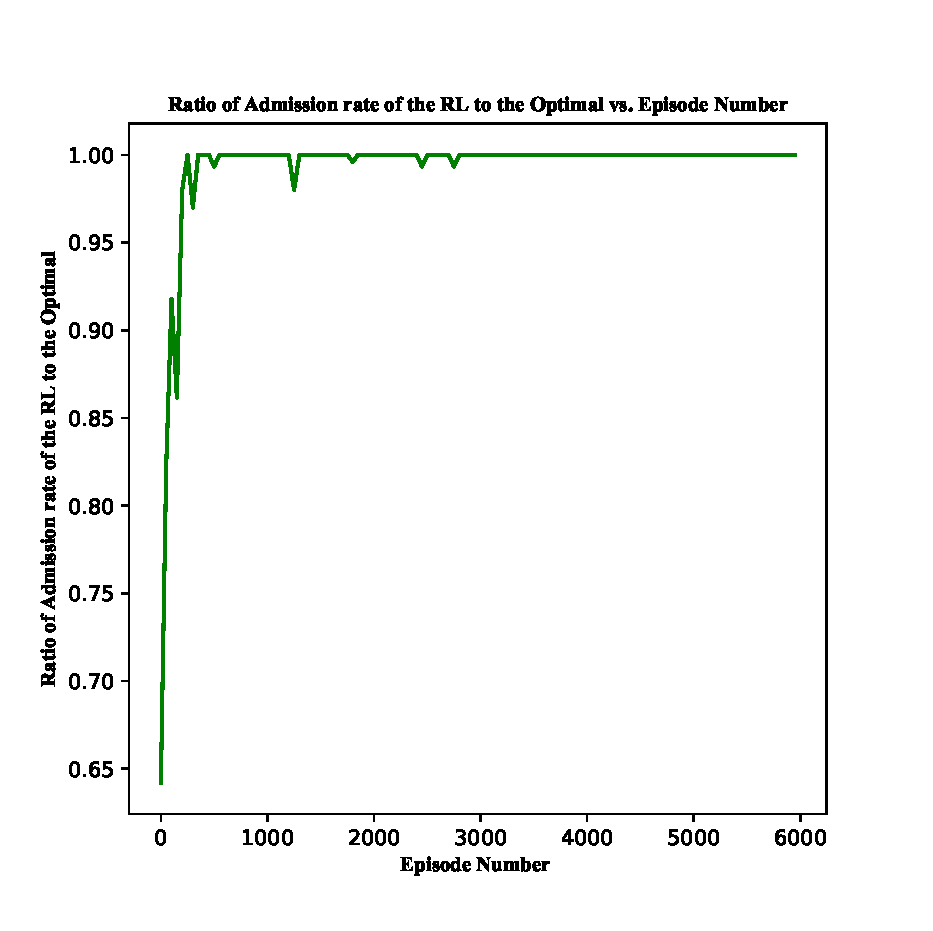
\includegraphics[scale = 0.6]{./fig/dynamicEpoch_0} %[width=\linewidth] 
	\caption{  نسبت تعداد سرویسهای پذیرفته شده با استفاده از روش یادگیری تقویتی عمیق به نسبت تعداد سرویسهای پذیرفته شده در حالت بهینه براساس زمان طی شده}
	\label{fig:dynamicEpoch}
\end{figure}
در شکل \ref{fig:dynamicEpoch1}
با افزایش تعداد برشها و بیشینه تعداد درخواستها در هر زمان، بعد از 1000 تکرار سناریو جواب به حالت بهینه نزیک شده ولی هیچ موقع با مقدار بهینه برابری نمی‌کند. در اینجا، تعداد درخواستهای سرویس اول 10 تا و سرویس دوم 5 تا می‌باشد. همچنین میزان خروج در هر بازه‌ی زمانی $80$ درصد سرویسهایی است که در حال پردازش هستند. % در اینجا هر سناریو 100 بار تکرار شده و میانگین گیری برروی آن انجام گردیده است.
\begin{figure}%[H]
	\centering
	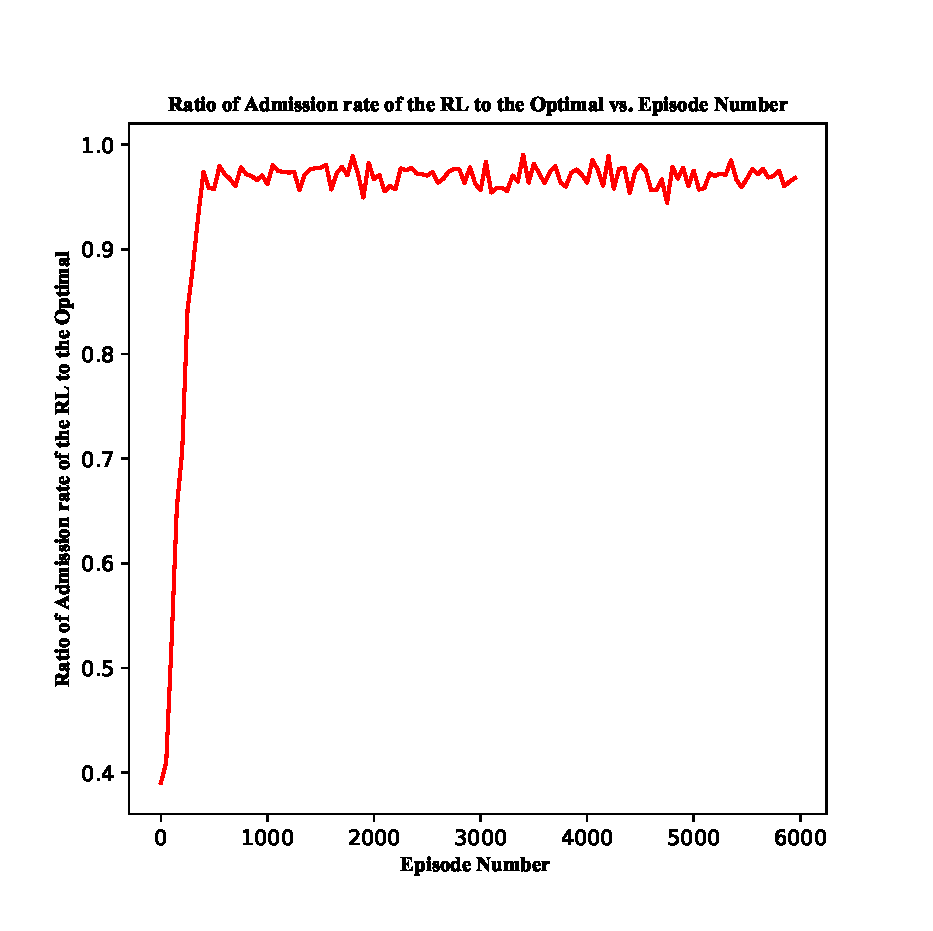
\includegraphics[scale = 0.6]{./fig/dynamicEpoch1_0} %[width=\linewidth] 
	\caption{  نسبت تعداد سرویسهای پذیرفته شده روش استفاده شده به نسبت تعداد سرویسهای پذیرفته شده در حالت بهینه براساس زمان طی شده با افزایش تعداد ماکسیمم درخواستها و تعداد برشهای شبکه}
	\label{fig:dynamicEpoch1}
\end{figure}
در شکل \ref{fig:admittedService}
با افزایش تعداد برشهای شبکه و به همان نسبت تعداد درخواستها، مقدار نرمالیزه‌ی میانگین مجموع تعداد سرویسهای پذیرفته شده‌ی هر دو نوع سرویس براساس  تعداد برشهای شبکه در دو حالت استفاده از روش بهینه و روش یادگیری تقویتی رسم شده است. با افزایش تعداد درخواستها و تعداد برشها، روش بهینه از روش یادگیری تقویتی فاصله می‌گیرد.

\begin{figure}%[H]
	\centering
	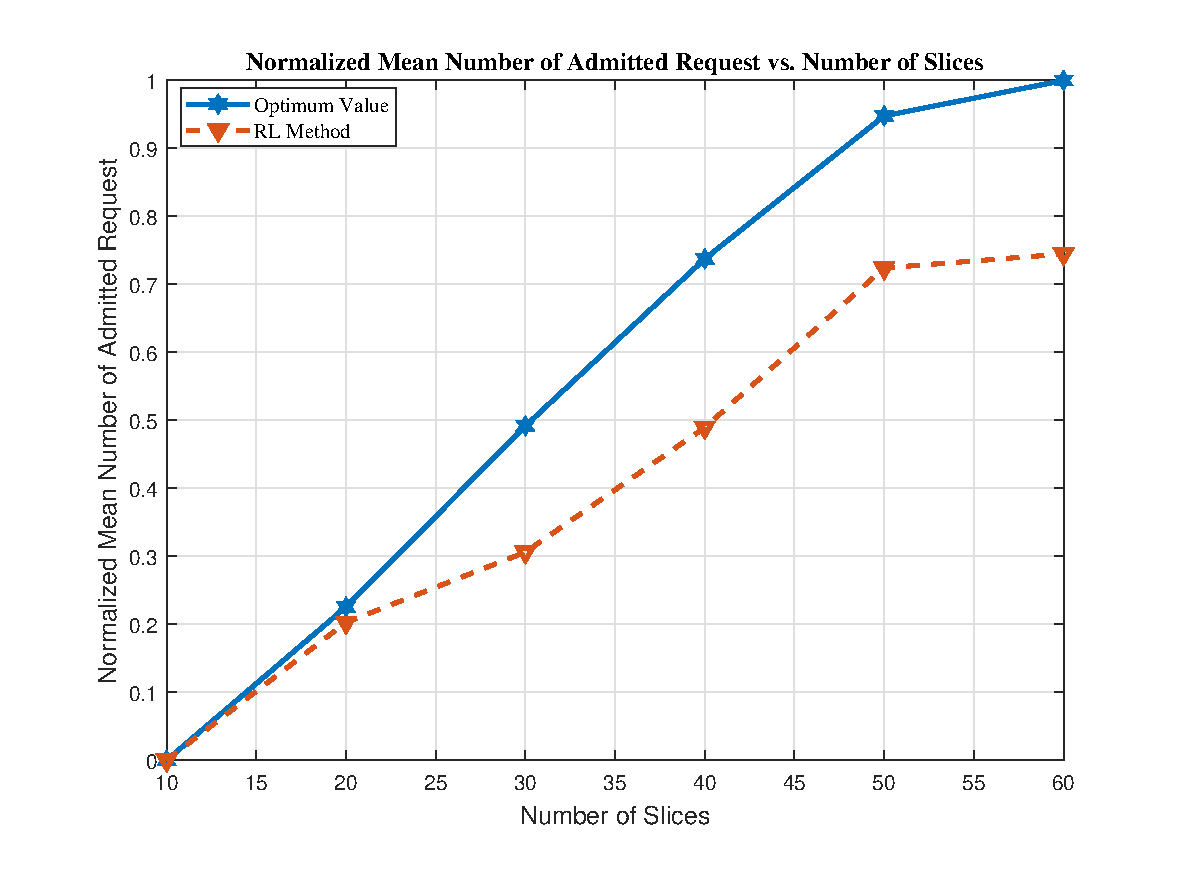
\includegraphics[scale = 0.6]{./fig/admittedService11} %[width=\linewidth] 
	\caption{  
		میانگین تعداد سرویسهای پذیرفته شده در زمان در دو حالت بهینه و استفاده از الگوریتم تقویتی با افزایش تعداد برشهای شبکه}
	\label{fig:admittedService}
\end{figure}
\subsection{نتایج عددی مسئله‌ی دوم} 
در این بخش، برای مسئله‌ی دوم حالت، عامل و پاداش را تعیین می‌نماییم و سپس نتایج عملی را نشان می‌دهیم.
در این مسئله، عامل، هماهنگ‌‌ ‌ساز است که وظیفه‌ی مدیریت شبکه را برعهده دارد.
همچنین، حالت در هر بازه‌ی زمانی برشهایی از شبکه است که به مراکزداده متصل شده و اینکه کدام برش به کدام مرکز داده متصل است.
پاداش طوری تعیین شده که کمترین تعداد مراکز داده استفاده گردد و هر لحظه کمترین تعداد مرکز داده‌ی خاموش، روشن شود.
در اینجا با فرض داشتن دو مدل سرویس مسئله را شبیه سازی می کنیم. فرض کنید VNF های سرویس اول نیاز به 
\lr{1 CPU}
و سرویس دوم نیازمند 
\lr{2 CPU}
است.
فرض کنید از سرویس اول ماکسیمم 6 تا درخواست VNF 
و برای سرویس دوم ماکسیمم در هر لحظه‌ی زمانی 4 تا درخواست VNF صورت می‌گیرد.
در این مسئله، تعداد زیادی سرور که دارای 3 تا CPU هستند در نظر گرفته شده است.
نسبت تعداد سرورهای مصرفی بهینه به سرورهای مصرفی با روش Q-learning  در شکل
\ref{fig:dynamicEpoch2}
نشان داده شده است.
\begin{figure}%[H]
	\centering
	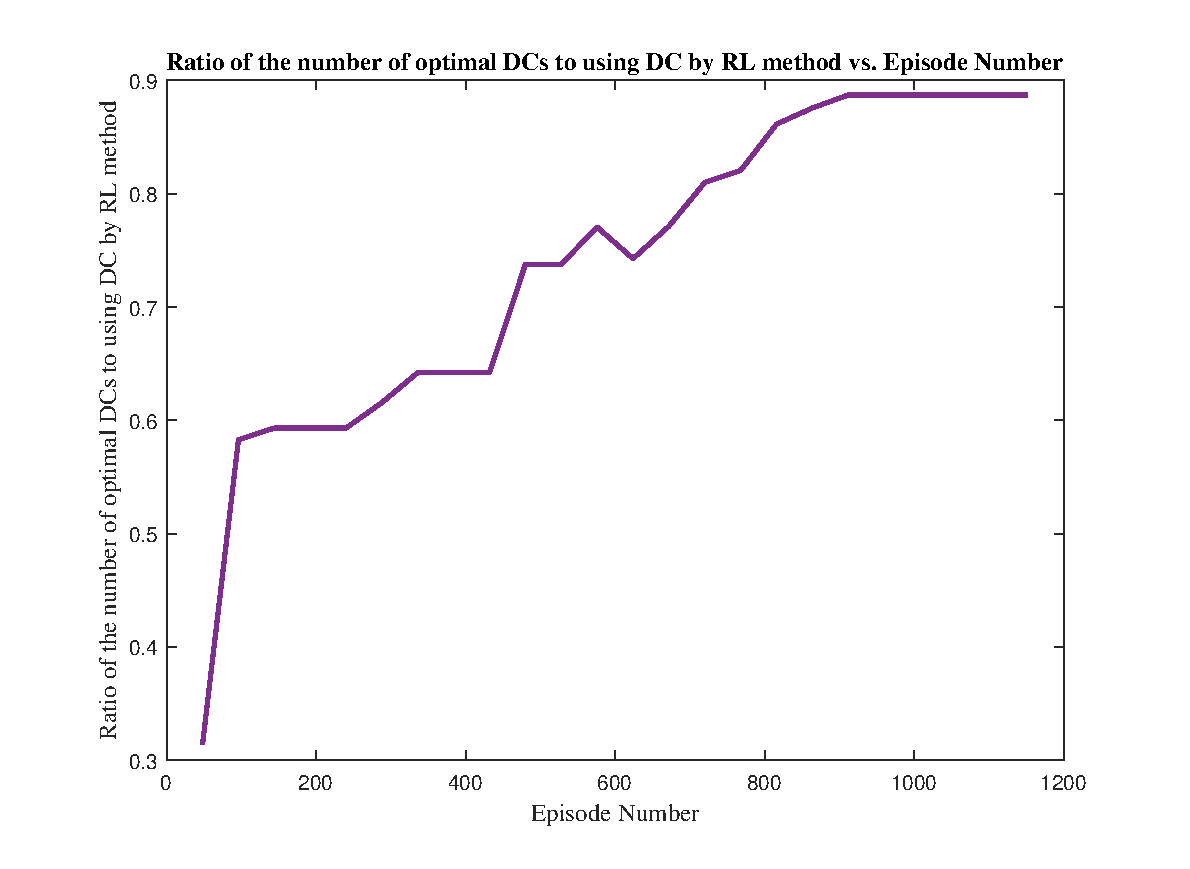
\includegraphics[scale = 0.6]{./fig/ratio_episode2} %[width=\linewidth] 
	\caption{   نسبت تعداد سرورهای مصرفی با روش 
		بهینه
		 به سرورهای مصرفی با استفاده از روش یادگیری تقویتی براساس زمان طی شده}
	\label{fig:dynamicEpoch2}
\end{figure}
همانطور که دیده می‌شود بعد از 900
تا تکرار، تقریبا به مقدار بهینه نزدیک شده‌ایم.
بعد از 900 تا تکرار سناریو، تقریبا میزان انتخاب عمل رندم به صفر رسیده و عمل بهینه از روی جدول Q بدست می‌آید.
%در اینجا هر سناریو 100 بار تکرار شده و میانگین گیری برروی آن انجام گردیده است. 
میزان خروج در هر بازه‌ی زمانی $80$ درصد مقدار سرویسهایی است که در زمان قبل در سیستم حضور داشتند، فرض شده است.
\begin{figure}%[H]
	\centering
	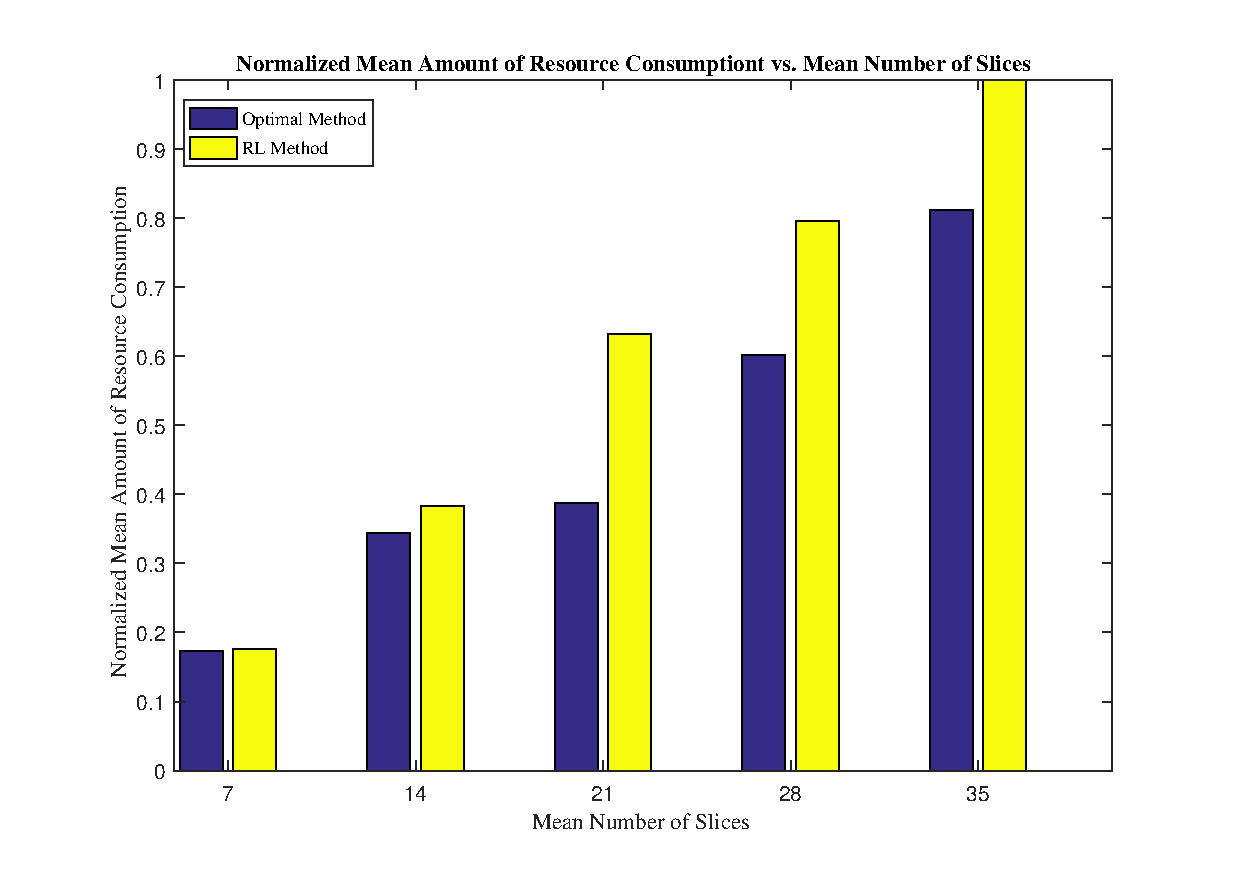
\includegraphics[scale = 0.6]{./fig/consumptionE} %[width=\linewidth] 
	\caption{  نسبت مقدار هزینه‌ی مصرفی نرمالیزه شده به تعداد میانگین برشهای مورد نیاز در جالت بهینه و الگوریتم یادگیری تقویتی }
	\label{fig:consumptionE}
\end{figure}
در شکل \ref{fig:consumptionE}
نسبت مقدار هزینه‌ی مصرفی نرمالیزه شده به تعداد میانگین برشهای مورد نیاز در جالت بهینه و الگوریتم یادگیری تقویتی رسم شده است. در اینجا با افزایش تعداد درخواستهای برشهای شبکه به منبع پردازشی به صورت میانگین، میزان هزینه‌ی مصرفی را در حالت بهینه و روش یادگیری تقویتی رسم کردیم و با افزایش درخواستها، روش یادگیری تقویتی از روش بهینه فاصله می‌گیرد. 
\section{نتیجه‌گیری}
در این فصل، دو مسئله‌ی فصل قبلی به صورت ساده شده نوشته شد و مسئله‌ی اول در بخش رادیویی از جنس کوله‌پشتی و مسئله‌ی دوم در بخش هسته از نوع 
بسته‌بندی جعبه می‌باشد. این دو مسئله به صورت دینامیکی در هر لحظه از زمان حل شده‌اند. برای حل این دو مسئله از روش یادگیری تقویتی  استفاده شده و حالتها و اعمال بیان برای یک عامل در این مسئله بیان گرده است.
نتایج عملی آن نیز رسم گردید. در هردو مسئله‌، به دلیل گسسته بودن اعمال و حالات مسئله و کم بودن تعداد آن از روش Q-learning
استفاده نمودیم. در مسئله‌ی اول ابتدا با فرض تعداد کمتر مسئله بعد از تعدادی تکرار به مقدار بهینه می‌رسد. با افزایش درخواستها از مقدار بهینه تا حدی دور می‌گردد. در مسئله‌ی دوم نیز بعد از 900 تکرار و با استفاده از جدول Q به مقدار نسبتا بهینه میل می‌کند.

  		% فصل چهارم: نتایج
\chapter{پیشنهادات و کارهای آتی}
\section{مقدمه}
در فصل اول، مقدمه‌ای بر مفاهیم مورد استفاده را بیان کردیم و در مورد نسل پنجم مخابرات و مفاهیم آن صحبت نمودیم. سپس در فصل دوم مروری بر کارهای انجام شده کردیم و مقالات مرتبط با برش شبکه و شبکه‌های دسترسی باز و قرارگیری توابع مجازی شبکه را بیان نمودیم تا مروری بر چالشهای مطرح شده نسل پنجم مخابرات کرده و حل این چالشها را مورد بررسی قرار دادیم . در فصل سوم صورت مسئله‌ای در زمینه‌ی برش شبکه در شبکه‌های دسترسی باز، معرفی کرده و با روش ابتکاری، آن را حل نمودیم و نتایج را با مقدار بهینه مقایسه کردیم.
در  فصل چهارم، دو مسئله‌ی بیان شده در فصل سوم را به صورت کاملا ساده با روش یادگیری عمیق تقویتی به صورت دینامیکی و در هر بازه‌ی زمان حل نمودیم. این دو مسئله، MDP \LTRfootnote{Markov Decision Processs}
بوده و قابل حل با این روش هستند. 
حال در این فصل در مورد مزایا و معایب کارهای انجام شده در فصل سوم و چهارم صحبت کرده و کارهای آتی و پیشنهادات را بیان می‌کنیم.
\section{نتیجه‌گیری}
در اینجا، مسئله‌ی برش شبکه در بخش رادیویی و قرارگیری توابع مجازی شبکه برروی مراکز داده باهم مورد بررسی قرار گرفته شد.
برای حل این مسئله، ابتدا مسئله به دو بخش مختلف شکسته شد که در بخش اول، تخصیص برش شبکه به کاربران سرویسها و تخصیص توان حل شده و پس از آن، برشهایی از شبکه که به سرویس اختصاص داده شده را به مراکز داده نگاشت می‌دهیم.
در این مسئله، تاخیر و نرخ هر کاربر در سرویس مورد بررسی قرار گرفته شده و چالش تخصیص منابع که شامل برش بخش رادیویی به هر سرویس است و جاگیری توابع شبکه حل می‌شود.
 الگوریتم ارائه شده سرعت بسیار بیشتری از الگوریتم بهینه که با MOSEK و CVX بدست می‌آید، دارد.
 سپس مسئله به صورت ساده‌تر برای حالت دینامیکی با روش یادگیری تقویتی حل گردیده است. 
 \subsection{مزایای این چالش و حل آن}
 در مسئله‌ی بیان شده‌ی فصل سوم، مدل سیستم به صورت دقیق بیان شده و نرخ کاربر، ظرفیت لینک fronthaul و تاخیر به طور دقیق مورد بررسی قرار گرفته شده است. همچنین مسئله به واقعیت نزدیکی زیادی دارد. همچنین الگوریتم ابتکاری تعریف شده در فصل سوم برای حالتی که تداخل به نسبت کم باشد به حالت بهینه بسیار نزدیک است. در فصل چهارم همین مسئله با فرض اینکه سرویسها نیازمند تاخیر کم یا نرخ بالا هستند به صورت پارامتریک در هر لحظه از زمان حل می‌گردند. 
 در بخش بعدی چالشهای قرارگیری توابع مجازی برروی مراکز داده به طور دقیق بررسی شده و ‌در فصل چهارم این مسئله به صورت دینامیکی در هر لحظه حل گردیده است. در حل مسئله در حالت دینامیکی سعی براین است که مراکز داده کمترنی انرژی را مصرف نموده و از هدر رفت انرژی بپرهیزیم.
 \subsection{معایب  پروژه انجام شده}
 در فصل سوم از الگوریتم ابتکاری در این کار استفاده شده است. زمانی که تعداد بلوکهای منابع فیزیکی به نسبت کاربران بسیار کم باشد و تداخل به شدت زیاد گردد، الگوریتم مسئله‌ی اول به خوبی قادر به پاسخ‌گویی نیست و از حالت بهینه فاصله ‌می‌گردد. در مسئله‌ی دوم، زمانی که تعداد مراکز داده زیاد گردد فاصله‌ی حالت بهینه از الگوریتم ابتکاری زیاد شده است. 
همچنین در فصل چهارم صورت مسئله بسیار ساده‌تر از واقعیت است و مسئله در حالت دینامیکی برای تعداد درخواست کم در این حالت حل گردیده است.
 \subsection{نوآوری‌های این پروژه}
 در این پروژه، تخصیص توان و برش شبکه در شبکه‌های دسترسی باز مورد بررسی قرار گرفته است.
 ما مسئله‌ی اختصاص UE به خدمات، خدمات به برش‌ها و منابع فیزیکی بی سیم و همچنین مرکز داده به برش‌ها را به عنوان یک مشکل بهینه سازی فرمول‌بندی کرده‌ایم. سپس با ارائه‌ی روشهای ابتکاری، به حل آنها پرداختیم. در نهایت مسئله‌ی ساده شده را در حالت دینامیکی و متغیر با زمان حل کردیم.
 \section{پیشنهادات}
 
 در این بخش، پیشنهادات و کارهای آتی را بیان خواهیم کرد.
 \begin{itemize}
\item
 یکی از کارهای آتی، مدل کردن برش شبکه در ساختار شبکه‌ی دسترسی رادیویی باز و حل آن بوسیله‌ی روش یادگیری تقویتی عمیق می‌باشد. در فصل چهارم از این روش برای سیستم ساده شده استفاده گردیده و به دلیل کم بودن تعداد حالات با استفاده از روش یادگیری تقویتی حل شده و در فصل سوم نیز مدل سیستم بیان شده، یکی از کارهای بعدی این است که سیستم مدل فصل سوم را به سیستمهای رادیویی باز نزدیکتر کرده و
با روش یادگیری تقویتی عمیق حل نماییم. که در اینجا، بدست آوردن توان و ارتباط برش با سرویس از این روش بدست خواهد آمد. همچنین مقایسه‌ی روش یادگیری تقویتی عمیق و یادگیری تقویتی در اینجا نیز مورد توجه قرار خواهد گرفت.
\item 
یکی دیگر از کارهای آتی، بدست آوردن پارامترهای کیفیت سرویس QoS\LTRfootnote{Quality of Service}
در شبکه‌های دسترسی باز می‌باشد که شامل تاخیر انتها به انتها، میزان از دست دادن بسته ها\LTRfootnote{Packet Loss}،
قابلیت اطمینان و ... می‌باشد.
در اینجا می‌توان تاخیر را هم در بخش رادیویی هم در بخش هسته‌ی شبکه بدست آورد. 
همچنین،
به منظور نشان دادن نقش هوش در ORAN طرح مدیریت هوشمند منابع رادیویی را برای کنترل تراکم ترافیک و نشان دادن کارایی آن در یک مجموعه داده واقعی از یک اپراتور بزرگ بدست می‌آوریم.
\item 
شبکه تعریف شده توسط نرم افزار (SDN) و مجازی سازی عملکرد شبکه (NFV) فناوری های کلیدی امکان پذیر در شبکه های ارتباطی نسل پنجم (5G) برای قرارگیری برش های شبکه سفارشی در سطح سرویس در زیرساخت شبکه، بر اساس خواسته های منابع آماری برای تأمین کیفیت طولانی مدت خدمات (QoS) مورد نیاز می‌باشد. با این حال، بارهای ترافیکی در برش های مختلف با گذشت زمان تحت تغییر قرار می‌گیرند ، در نتیجه چالش هایی برای تأمین کیفیت مداوم ایجاد می‌شود.
در کارهای آتی یک مشکل انتقال جریان پویا برای سرویس های متصل شده به برش شبکه، برای پاسخگویی به نیازهای تأخیر پایان انتها به انتها (E2E) با ترافیک متغیر، مورد بررسی قرار خواهد گرفت.
\item
یکی دیگر از کارهای آتی، تخصیص منابع به روش توزیع شده برای برش شبکه از منابع محاسباتی و منابع دیگر همانند پهنای باند می‌باشد.
همچنین از روش توزیع شده در لینک فراسو  
\LTRfootnote{Uplink}
برای تخصیص توان کاربران، تخصیص پهنای باند و ... استفاده می‌گردد. یکی از روشها، استفاده از 
\lr{Distributed ADMM}
می‌باشد که در این روش تعدادی عامل به صورت همکارانه سعی در حل یک معادله‌ی بهینه‌سازی مشترک دارند که تابع هدف مجموعی از مقدارهای خصوصی هر عامل ‌می‌باشد. 
 \end{itemize}
 
  		% فصل پنجم: بحث و نتیجه‌گیری

% مراجع
% اگر از استیل‌های natbib استفاده می‌کنید باید دو خط را در فایل commands.tex تغییر دهید.
\pagestyle{empty}
{
\small
\onehalfspacing
%\bibliographystyle{plain-fa} % or plainnat-fa for author-date


\begin{latin}
\bibliographystyle{IEEEtran}
\renewcommand{\bibname}{\rl{{کتاب‌نامه}\hfill}} 
\bibliography{tehran-thesis/tex/MyReferences}
\end{latin}
}

\pagestyle{fancy}

% \appendix
% فصلهای پس از این قسمت به عنوان ضمیمه خواهند آمد.

% دستورات لازم برای تبدیل «فصل آ» به «پیوست آ» در فهرست مطالب 
\addtocontents{toc}{
    \protect\renewcommand\protect\cftchappresnum{\appendixname~}%
    \protect\setlength{\cftchapnumwidth}{\mylenapp}}
    
\let\Chapter\chapter
% دستورات لازم برای شماره‌گذاری صفحات پیوست‌ها بشکل آ-۱ (فعلا با glossaries سازگار نیست)
%\pretocmd{\chapter}{
%  \clearpage
%  \pagenumbering{arabic}
%  \renewcommand*{\thepage}{\rl{\thechapter-\arabic{page}}}}{}{}
%%%%%%%%%%%%%%%%%%%%%%%%%%%%%%%%%%%%%
    

\include{./tex/appendix1}		% پیوست اول: آشنایی مقدماتی با لاتک
\include{./tex/appendix2}		% پیوست دوم: جدول، نمودار و الگوریتم در لاتک
\include{./tex/appendix3}   	% پیوست سوم: مراجع، واژه‌نامه و حاشیه‌نویسی

% برگرداندن شماره‌بندی صفحات فصول
\let\chapter\Chapter
\pagenumbering{tartibi} % اول، دوم، ...
%\baselineskip=.75cm

% چاپ واژه‌نامه‌ها و نمایه 
\onehalfspacing
\printglossary
\printindex

\begin{latin}
\baselineskip=.6cm
\latinTitlePage
\end{latin}
\label{LastPage}

\end{document}